\documentclass[12pt]{scrreprt}

\usepackage[utf8]{inputenc}
\usepackage{ngerman, url}
\usepackage{hyperref}
\usepackage{microtype}
\usepackage{tikz}
\usepackage{schnaubelt}

\author{Die Mitarbeiter von \url{http://mitschriebwiki.nomeata.de/}}
\title{Analysis I}
\makeindex


\begin{document}
\maketitle

\tableofcontents

\setcounter{chapter}{-1}
\chapter{Vorbemerkungen}
\label{cha:vor}

\section{Bezeichnungen}
\label{sec:vor.bezeichnungen}
\subsection*{Allgemeine Bezeichnungen}

\begin{itemize}
\item griechische Buchstaben: s. Übungsblatt.
\item Thm = Theorem = Hauptsatz.
\item Def. = Definition, "`{\da}"' heißt "`steht für"'.
\item Lem. = Lemma = Hilfssatz.
\item Bew. = Beweis.
\item Beh. = Behauptung.
\item Ann. = Annahme.
\item n.V. = nach Voraussetzung.
\item Vor. = Voraussetzung.
\item Bsp. = Beispiel.
\item Bem. = Bemerkung.
\item $\Box$ = Beweisende.
\end{itemize}

\subsection*{Logische Symbole}
\begin{itemize}
\item $\neg$ = nicht.
\item $\wedge$ = und.
\item $\vee$ = oder.
\item $\ra$ = impliziert.
\item $\Longleftrightarrow$ = equivalent.
\item $\forall$ = für alle.
\item $\exists$ = es existiert.
\item $\exists!$ = es existiert genau eines.
\end{itemize}

\subsection*{Etwas zu Mengen}
Mengen werden durch die Angabe ihrer Elemente definiert, z.\,B. $M = \{1, 2, 3\} = \{2, 1, 3\} =$ die Menge, die aus 1, 2 und 3 besteht.
\begin{itemize}
\item $M = \set{N} =$ die Menge der natürlichen Zahlen.
\item $M = \{\nat{x}: x$ ist gerade\} = gerade Zahlen.
\item $\emptyset$ = leere Menge = $\{\}$.
\end{itemize}

\subsection*{Operationen mit Mengen $M,\ N$:}
\begin{itemize}
\item $x \in M$ -- "`$x$ ist ein Element von M."' (Beispiel: $1 \in \{1, 2, 3\}$)
\item $x \notin M$ -- "`$x$ ist kein Element von M."'
\item $M \subseteq N$ -- "`M ist Teilmenge (TM) von M,"' d.\,h. wenn $x \in M$, dann auch $x \in N$, \emph{oder}: $x \in M \folgt x \in N$.
\item $M = N$ -- "`$M \subseteq N$ und $N \subseteq M$"' \emph{oder}: $M$ und $N$ haben die gleichen Elemente.
\item $M \cap N = \{x: x \in M$ und $x \in N\}$ = Schnittmenge = Menge der $x$, die in beiden Mengen liegen.
\item $M \cup N = \{x: x \in M$ oder $x \in N\} =$ Vereinigungsmenge = Menge der $x$, die in einer der beiden Mengen liegen (oder auch in beiden).
\item $M \times N = \{(x,y): x \in M$, $y \in N\} =$ Menge der geordneten Paare aus $M$ und $N$. Ferner: $M^2 = M \times M$, $M^n = M \times \dotsb \times M$ ($n$-fach) (\nat{n}).
\item $M \setminus N = \{x \in M: x \notin N\} =$ Differenzmenge = Menge der $x$ aus $M$, die nicht in $N$ liegen.
\item $\mathcal{P}(M) = \{N: N \subseteq M\} =$ Potenzmenge = die Menge aller Teilmengen von $M$.
\item $\mathcal{P}(\{1, 2, 3\}) = \{\emptyset, \{1\}, \{2\}, \{1, 2\}, \{2, 3\}, \{1, 3\}, \{1, 2, 3\}\}$. Zugehörige Rechenregeln, siehe LA.
\end{itemize}

\subsection*{Abbildungen (Abb.) oder Funktionen (Fkt.):}
Seien $M$ und $N$ Mengen. Eine Funktion $f: M \ra N,\ x \mapsto f(x)$ besteht aus dem Definitions\-bereich $M$, dem Bildbereich $N$ und der Abbildungsvorschrift $f$, die jedem "`Urbild"' $x \in M$ genau ein "`Bild"' $f(x) \in N$ zuordnet.
Streng genommen ist die Funktion das Tripel $(f, M, N)$, man schreibt meistens nur $f$. Beispiel: $f: \set{N} \ra \set{N},\ x \mapsto 2x$. Hier schreibt man auch $f: \set{N} \ra \set{N}$, $f(x) = 2x$.

\section{Vollständige Induktion}
\label{sec:vor.vollstInd}
Wir setzen die natürlichen Zahlen $\set{N} = \{1, 2, 3, \dotsc\}$, ($\set{N}_0 = \{0, 1, 2, \dotsc\}$), die ganzen Zahlen $\set{Z}$ und die Brüche $\set{Q}$ samt ihren Rechenregeln vorraus.

Dann gilt das \emph{Prinzip der vollständigen Induktion} (vollst. Ind.).

\noindent $M \subseteq \set{N}$ erfülle die beiden folgenden Bedingungen:

\noindent (IA) $1 \subseteq M$

\noindent (IS) Wenn ein $\nat{n}$ zu $M$ gehört, dann gehört auch der Nachfolger $n + 1$ zu $M$.

\noindent\emph{Beh.} Dann gilt $M = \set{N}$.
\begin{proof}[Beweis (indirekt)]
\emph{Annahme} Die Behauptung sei falsch. Dann existiert ein $\nat{m} \setminus M$. Nach (IA) ist $1 \in M$. Dann liefert (IS), dass $2 = 1 + 1 \in M$. Diesen Schritt wiederholt man $(m - 1)$ mal. Somit erhält man mit $\nat{m}$ einen Widerspruch ($\blitz$) zu $\nat{m} \setminus M$. Also muss die Annahme falsch sein, d.\,h. die Behauptung ist wahr.
\end{proof}

\noindent Eine \emph{Aussage} ist ein "`Satz"', der entweder wahr oder falsch ist, z.\,B. $7 + 5 = 12$, $3 + n = n$ sind Aussagen.
$n + 1$ ist keine Aussage.

\subsection*{Beweisprinzip der vollständigen Induktion}
Es seien für jedes $\nat{n}$ Aussagen $A(n)$ gegeben. Wir wollen zeigen, dass alle Aussagen wahr sind, d.\,h. $M \da \{\nat{n}: A(n)$ ist wahr$\}$ muss gleich $\set{N}$ sein. Nach dem Prinzip der vollständigen Induktion muss man also die folgenden Behauptung zeigen:

\begin{enumerate}
\item[(IA)] Induktionsanfang: Man zeigt, dass $A(1)$ wahr ist.
\item[(IS)] Induktionsschluss: Es gelte die Induktionsvoraussetzung (IV): Für ein (festes, aber beliebiges) $\nat{n}$ ist $A(n)$ wahr.
\end{enumerate}

\noindent Dann zeigt man, dass auch $A(n+1)$ wahr ist.
Dann folgt, dass alle $A(n)$ wahr sind.

\begin{bsp}\label{bsp:vor.gauss}
Zeige: $1 + 2 + 3 + \dotsb + n = \frac{1}{2}n(n+1)$, $\forall \nat{n}$.
\begin{proof}[Beweis (per vollst. Ind.)]
Es sei $A(n): 1 + \dotsb + n = \frac{1}{2}n(n+1)$, $\nat{n}$.

\noindent IA: $n = 1: 1 = \frac{1}{2}\cdot 1 \cdot 2 \folgt A(1)$ ist wahr.

\noindent IS: Es gelten $A(n)$ für ein $\nat{n}$ (IV).

\noindent Dann: $(1+ \dotsb + n) + n+1 \nach{=}{(IV)} \frac{1}{2}n(n+1) + (n+1)\cdot\frac{1}{2}\cdot 2 = \frac{1}{2}(n+1)(n+2)$

\noindent \folgt $A(n+1)$ ist wahr. \folgt IS ist gezeigt. \folgt Beh. nach vollst. Ind. 
\end{proof}

\noindent Unbefriedigend ist die Schreibweise "`$+\dotsb +$"', dafür: "`rekursive Def."' des Summenzeichens:
Gegeben seien $\rat{a_j}$ für jedes $\zahl{j}$ mit $j \geq m$ für ein festes $\zahl{m}$. Dann setzen wir:
\[\sum_{j=m}^m a_j \da a_m.\]

\noindent Wir nehmen an, dass $\displaystyle \sum_{j=m}^{m+n} a_j$ für ein festes, aber beliegiges $\nat{n}$ definiert sei.
Dann definieren wir:
\[\sum_{j=m}^{m+n+1} a_j \da \left( \sum_{j=m}^{m+n} a_j\right) + a_{m+n+1}.\]

\noindent Nach dem Induktionsprinzip ist die Menge: $\displaystyle M = \{\nat{n}: \sum_{j=m}^{m+n} a_j$ ist def.$\}$ gleich $\set{N}$. (Korrektur: Hier braucht man das Induktionsprinzip für $\set{N}_0 = \{0, 1, 2, \dotsc\}$, siehe Übung.)

Wir haben also den Ausdruck $\displaystyle \sum_{j=m}^k a_j$ für alle $\zahl{k}$, $k \geq m$ definiert.
Man schreibt oft $\displaystyle \sum_{j=m}^k a_j = a_m + \dotsb + a_k$.
Genauso definiert man: $\displaystyle \prod_{j=m}^k a_j = a_m \cdot a_{m+1}\dotsm  a_k$.

\noindent Es gelten die üblichen Rechenregeln, wie man per Induktion zeigt. Dazu ein Beispiel, wobei $m = 1$.
Gegeben seien $a_j$, $b_j\in\set{Q}$, $\nat{j}$. Dann gilt:
\[A(n): \sum_{j=1}^n a_j + \sum_{j=1}^n b_j = \sum_{j=1}^n (a_j + b_j),\quad\forall \nat{n}.\]

\begin{proof}[Beweis (per Ind.)]
\begin{enumerate}
\item[IA:] $\displaystyle n = 1: \sum_{j=1}^1 a_j + \sum_{j=1}^1 b_j \nach{=}{Def.} a_1 + b_1 \nach{=}{Def.} \sum_{j=1}^1 (a_j + b_j)$ \folgt $A(1)$ ist wahr.
\item[IS:] Es gelte $A(n)$ für ein $\nat{n}$ (IV). Dann:
\[\sum_{j=1}^{n+1} a_j + \sum_{j=1}^{n+1} b_j \nach{=}{Def.} \left(\sum_{j=1}^n a_j + a_{n+1}\right) + \left(\sum_{j=1}^n b_j + b_{n+1}\right)\]
\[\nach{=}{Def.} \sum_{j=1}^n (a_j + b_j) + (a_{n+1} + b_{n+1}) \nach{=}{Def.} \sum_{j=1}^{n+1} (a_j + b_j).\]
\end{enumerate}
\noindent\folgt $A(n+1)$ ist wahr. \folgt IS gilt. \folgt $A(m)$ gilt $\forall \nat{m}$.
\end{proof}
\end{bsp}

\begin{bsp}[Geometrische Summenformel]\label{bsp:vor.geomet-summe} 
Gegeben sei $\rat{q}\setminus \{1\}$.\\ \emph{Beh.} Dann gilt:
\[A(n): \sum_{j=0}^n q^j = \frac{q^{n+1}-1}{q-1},\ \forall\nat{n}.\]
\begin{proof}[Beweis (per Ind.)]
\begin{enumerate}
\item[IA:] $\displaystyle (n = 1): \sum_{j=0}^1 q^j = q^0 + q^1 = 1+q$,\\
$\displaystyle \frac{q^2 - 1}{q-1} = \frac{(q+1)(q-1)}{q-1} = 1+q$.
"`="' \folgt $A(1)$ ist wahr.
\item[IS:] Es gelte $A(n)$ für ein $\nat{n}$ (IV). Dann:
\[\displaystyle \sum_{j=0}^{n+1} q^j = \sum_{j=0}^n q^j + q^{n+1} \nach{=}{(IV)} \frac{q^{n+1}-1}{q-1} + q^{n+1} = \frac{q^{n+1}-1+q^{n+2}-q^{n+1}}{q-1} = \frac{q^{n+2}-1}{q-1}.\]
\end{enumerate}

\noindent\folgt $A(n+1)$ gilt \folgt (IS) ist gezeigt. 
\folgt Ind. zeigt, dass $A(n)$ für alle $\nat{n}$ gilt.
\end{proof}

\noindent Eine weitere rekursive Definition:

\noindent \emph{Fakultät}: $0! = 1$, $1! = 1$.
Wenn $n!$ für ein $\nat{n}$ definiert ist, dann setzt man $(n+1)! = (n+1)\cdot n!$.
Man schreibt: $n! = 1 \cdot 2 \dotsm n$.

\begin{dfn*}[Binomialkoeffizienten]
Seien $n$, $j\in\set{N}_0$ und $n \geq j$.
Dann setzt man 
\[\binom{n}{j} \da \frac{n!}{j!(n-j)!} = \frac{1\cdot 2\dotsm n}{(1\cdot 2\dotsm j)(1\cdot 2\dotsm (n-j))}.\]

\noindent Eigenschaften: ($n$, $j\in\set{N}_0$, $n \geq j$)
\begin{enumerate}
\item $\displaystyle\binom{n}{n-j} = \frac{n!}{(n-j)!(n-n+j)!} = \binom{n}{j}.$
\begin{equation}\label{eqn:vor.n-ueber-n}
\displaystyle\binom{n}{0} = \frac{n!}{0!n!} = 1 = \binom{n}{n}.
\end{equation}

\item Sei $j \geq 1$. Dann: $\displaystyle\binom{n}{j-1}+\binom{n}{j} = \frac{n!\cdot j}{(j-1)!(n-j+1)!\cdot j} + \frac{n!(n-j+1)}{j!\cdot(n-j)!(n-j+1)}$
\begin{equation}\label{eqn:vor.np1-ueber-j}
\nach{=}{Def. Fak.} \frac{j\cdot n! + (n-j+1)n!}{j!(n-j+1)!} \nach{=}{Def. Fak.} \frac{(n+1)!}{j!(n+1-j)!} \nach{=}{Def.} \binom{n+1}{j}
\end{equation}
\end{enumerate}
\end{dfn*}
\end{bsp}

\begin{bsp}[Binomischer Satz]\label{bsp:vor.binom}

Seien $a$, $b\in\set{Q}$, $\nat{n}$. Dann \[A(n):\ (a+b)^n = \sum_{j=0}^n\binom{n}{j}a^{n-j}b^j,\quad\nat{n}.\]
\begin{proof}[Beweis (per Ind.)]
\begin{enumerate}
\item[IA:] $(n=1)$
\[\sum_{j=0}^1\binom{1}{j}a^{1-j}b^j \nach{=}{(\ref{eqn:vor.n-ueber-n})} 1\cdot a^1\cdot b^0 + 1\cdot a^0\cdot b^1 = (a+b)^1.\]
$\folgt A(1)$ ist wahr.
\item[IS:] $A(n)$ gelte für ein $\nat{n}$ (IV).
\begin{align*}
(a+b)^{n+1} &= (a+b)(a+b)^n \nach{=}{(IV)} (a+b)\sum_{j=0}^n\binom{n}{j}a^{n-j}b^j\\
&= \sum_{j=0}^n\binom{n}{j}a^{n-j+1}\cdot b^j + \sum_{j=0}^n\binom{n}{j}a^{n-j}\cdot b^{j+1}\\
\text{setze }l = j+1&(\gdw j = l-1)\\
&=\sum_{j=0}^n\binom{n}{j}a^{n+1-j}\cdot b^j + \sum_{l=1}^{n+1}\binom{n}{l-1}a^{n+1-l}\cdot b^l\\
&\nach{=}{(\ref{eqn:vor.n-ueber-n})} \underbrace{a^{n+1}}_{(j=0)}\sum_{j=1}^n\underbrace{\left(\binom{n}{j}+\binom{n}{j-1}\right)}_{\nach{=}{(\ref{eqn:vor.np1-ueber-j})}\binom{n+1}{j}}\underbrace{a^{n+1-j}\cdot b^j}_{(j=l\text{ gesetzt})}+\underbrace{1\cdot a^0\cdot b^{n+1}}_{(j=n+1)}\\
&= \sum_{j=0}^{n+1}\binom{n+1}{j}a^{n+1-j}\cdot b^j
\end{align*}
\end{enumerate}
\noindent\folgt $A(n+1)$ ist gezeigt \folgt (IS) gilt.
\folgt Beh. folgt mit vollst. Ind.
\end{proof}
\end{bsp}

%%%%%%%%%%%%%%%%%%%%%%%%%%%%%%%%%%%%%%%%%%%%%%%%%%%%%%%%%%%%%%%%%%%%%%
\chapter{Reelle und komplexe Zahlen}
\label{cha:zahlen}
%%%%%%%%%%%%%%%%%%%%%%%%%%%%%%%%%%%%%%%%%%%%%%%%%%%%%%%%%%%%%%%%%%%%%%
Wir definieren die reellen Zahlen "`axiomatisch"', d.h.: Man legt in einer Definition die 
Eigenschaften der reellen Zahlen fest, die im folgenden verwendet werden dürfen.
Ausblick: \set{R} ist ein "`ordnungsvollständiger, geordneter Körper"'.

\section{Geordnete Körper}
\label{sec:zahlen.geordnete-koerper}
\begin{dfn*}
Sei $M$ eine nichtleere Menge. Eine Abbildung $\ast: M\times M \ra M(x, y) 
\mapsto x \ast y$ heißt Verknüpfung auf $M$.
\end{dfn*}

\begin{dfn}
\label{dfn:zahlen.koerper}
Seien $K$ eine Menge, $0 \in K$, $1 \in K$ mit $0 \ne 1$, und "`$+$"' und "`$\cdot$"' Verknüpfungen auf 
$K$. Dann heißt $(K, 0, 1, +, \cdot)$ ein \emph{Körper}, wenn die folgenden Eigenschaften für alle 
$x$, $y$, $z \in K$ gelten:

\begin{enumerate}
\item Assoziativgesetze:
\[(x + y) + z = x + (y + z)\]
\[(x \cdot y) \cdot z = x \cdot (y \cdot z)\]

\item neutrale Elemente:
\[x + 0 = x,\ x \cdot 1 = x\]

\item inverse Elemente:
\begin{itemize}
  \item Zu jedem $x \in K$ existiert ein $a \in K$ mit $x + a = 0$.
  \item Zu jedem $x \in K \setminus \{0\}$ existiert ein $b \in K$ mit $x \cdot b = 1$.
\end{itemize}

\item Kommutativgesetze:
\[x + y = y + x,\ x \cdot y = y \cdot x\]

\item Distributivgesetz:
\[(x + y) \cdot z = (x \cdot z) + (y \cdot z)\]
\end{enumerate}

Man schreibt oft $K$ anstelle $(K, 0, 1, +, \cdot)$.
\end{dfn}

\begin{bsp*}
\begin{enumerate}
\item \set{Q} mit den üblichen 0, 1, $+$, $\cdot$ ist ein Körper.
\item \set{Z} ist kein Körper, da es kein $b \in$ \set{Z} gibt mit $2b = 1$.
\item Weitere Beispiele in linearer Algebra und Analysis I.
\end{enumerate}
\end{bsp*}

\begin{bem*}
\begin{enumerate} % buchstaben
\item Wir schreiben $-x$ für das Inverse Element von $x \in K$ bzgl. der Addition und $\displaystyle x^{-1} = \frac{1}{x}$ für das Inverse Element von $x \in K \setminus \{0\}$. Man lässt "`$\cdot$"' und überflüssige Klammern meist weg. Dabei gilt "`$\cdot$"' vor "`$+$"'.

\item Die inversen Elemente sind eindeutig bestimmt (siehe LA). Man schreibt $x - y$ statt $x + (-y)$ und $\displaystyle\frac{x}{y}$ statt $x \cdot y^{-1}$.

\item Es gelten Rechenregeln wie in der Bruchrechnung (z.B. $0 \cdot x = 0$, $-(-x) = x$, usw.) [siehe LA]. Im folgenden wird dies ohne Kommentar in Ana I verwendet.
\end{enumerate}
\end{bem*}

\begin{dfn}\label{dfn:relation}
Sei $M$ eine nichtleere Menge. Eine \emph{Relation} $R$ auf $M$ ist eine Teilmenge von $M \times M$. Man schreibt $x \sim_R y$ statt $(x, y) \in R$.

$R$ ist \emph{Ordnungsrelation} (oder Ordnung), wenn gelten:
\begin{enumerate} % Buchstaben
\item $\forall x \in M: x \sim_R x$ (reflexiv).
\item $\forall x, y, z \in M:$ Wenn $x \sim_R y$ und $y \sim_R z$, dann auch $x \sim_R z$ (transitiv).
\item\label{dfn:relation.antisymm} $\forall x, y \in M:$ Wenn $x \sim_R y$ und $y \sim_R x$, dann gilt $x = y$ (antisymmetrisch). Statt $\sim_R$ schreibt man in diesem Fall meist $\leq_R$ oder $\geq_R$. Eine Ordnung heißt total, wenn für beliebige $x, y \in M$ stets $x \leq y$ oder $y \leq x$ gilt.
\end{enumerate}

Man schreibt $x < y$, wenn $x \leq y$ und $x \ne y$, sowie $x \geq y$ statt $y \leq x$ und $y > x$ statt $x < y$.

\begin{bsp*}
\begin{enumerate} %Buchstaben
\item Die übliche Ordnung auf $\set{Q}$ erfüllt Definition~\ref{dfn:relation} und ist total. Hier:

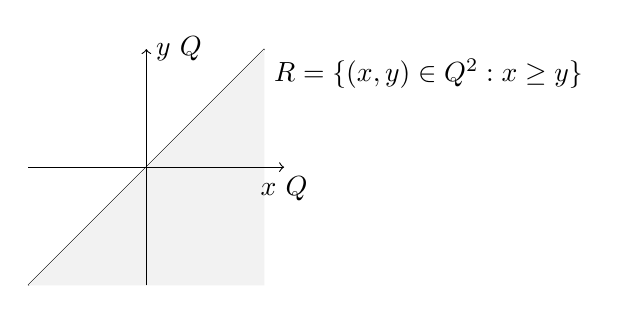
\begin{tikzpicture}
  \draw (-1.5,-1.5) -- (1.5,1.5) node[below right] {$R = \{(x,y) \in \set{Q}^2: x \geq y\}$};
  \fill [black!5!white] (1.5,1.5) -- (1.5,-1.5) -- (-1.5,-1.5) -- cycle;

  \draw[->] (-1.5,0) -- (1.75,0) node[below] {$x\ \set{Q}$} coordinate (x axis);
  \draw[->] (0,-1.5) -- (0,1.5) node[right] {$y\ \set{Q}$} coordinate (y axis);
\end{tikzpicture}

\item Die Relation "`$n$ teilt $m$"' für $n, m \in M$ ist eine \emph{nicht-}totale Ordnung, z.B. $2$ und $3$ teilen sich nicht.
\end{enumerate}
\end{bsp*}
\end{dfn}

\begin{dfn}\label{dfn:geordn.koerper}
Ein \emph{geordneter Körper} $K = (K,\ \leq)$ besteht aus einem Körper $K$ und einer \emph{totalen} Ordnung $\leq$, sodass die folgenden Eigenschaften gelten:
\begin{enumerate} % eigentlich 01, 02 ...
\item\label{dfn:geordn.koerper.01} $\forall x, y, z \in K:$ Wenn $x < y$, dann $x + z < y + z$.
\item\label{dfn:geordn.koerper.02} $\forall x, y \in K:$ Wenn $x > 0$ und $y > 0$, dann gilt $xy > 0$.
\end{enumerate}

$x \in K$ heißt \emph{positiv} (\emph{negativ}), wenn $x \geq 0$ ($x \leq 0$). $x \in K$ heißt \emph{strikt positiv} (\emph{strikt negativ}), wenn $x > 0$ ($x < 0$). Man setzt

\[K_+ = \{x \in K: x \geq 0\},\ K_- = \{x \in K: x \leq 0\}\]
\end{dfn}

\medskip\noindent\makebox[.25\textwidth]{\hrulefill}\medskip % kleine Linie?!

% hier sollte die reference allerdings ein Buchstabe und keine Zahl sein :-/
Es gelten $K_+ \cap K_- = \{0\}$ (nach Def. \ref{dfn:relation}~{\ref{dfn:relation.antisymm}}), sowie $K_+ \cup K_- = K$ (wegen der Totalität).

\begin{bsp*}
$\set{Q}$ mit der üblichen Ordnung ist ein geordneter Körper.
\end{bsp*}

\begin{satz}\label{satz:geordn.koerper}
\begin{enumerate} % Buchstaben
\item $y > x \gdw y - x > 0$.
\item\label{satz:geordn.koerp.b} \begin{enumerate}% i, ii
	\item $x < 0 \gdw -x > 0$.
	\item $x > 0 \gdw -x < 0$.
\end{enumerate}
\item Wenn $x > 0$ und  $y < 0$, dann $xy < 0$.
\item Wenn $x \neq 0$, dann $x^2 = x \cdot x > 0$. Speziell: $1 = 1^2 > 0$.
\item Wenn $x > 0$, dann $\displaystyle\frac{1}{x} > 0$.
\end{enumerate}
\end{satz}

\begin{proof}
\begin{enumerate} %Buchstaben
\item\label{bew:geordn.koerp.a} Sei $y > x$. Addiere $-x$ zu beiden Seiten. \ref{dfn:geordn.koerper}~\ref{dfn:geordn.koerper.01} liefert $y - x > x - x = 0$.

Sei $y - x > 0$. Addiere $x$. \ref{dfn:geordn.koerper}~\ref{dfn:geordn.koerper.01} $\folgt y = y - x + x > x$.

\item\label{bew:geordn.koerp.b} \begin{enumerate} % i, ii
	\item\label{bew:geordn.koerp.b.i} Setze $y = 0$ in \ref{bew:geordn.koerp.a}.
	\item Ergibt sich, wenn man in \ref{bew:geordn.koerp.b.i} $x$ durch $-x$ ersetzt.
  
	(Beachte: $-(-x) = x$).
\end{enumerate}

\item Seien $x > 0$, $y < 0 \stackrel{\ref{bew:geordn.koerp.b}}{\folgt} -y > 0 \stackrel{\ref{dfn:geordn.koerper}~\ref{dfn:geordn.koerper.02}}{\folgt} 0 < x \cdot (-y) = -xy \stackrel{\ref{bew:geordn.koerp.b}}{\folgt} xy < 0$.

\item\label{bew:geordn.koerp.d} Sei $x + 0$. Nach \ref{bew:geordn.koerp.b} und der Totalität der Ordnung gilt entweder $x>0$ oder $-x>0$. \ref{bew:geordn.koerp.d} folgt also aus \ref{dfn:geordn.koerper}~\ref{dfn:geordn.koerper.02} und $(-x)^2 = x^2$.

\item Sei $x>0$. \emph{Ann.} $\displaystyle\frac{1}{x} < 0$. Dann $\displaystyle-\frac{1}{x} > 0$ (nach \ref{bew:geordn.koerp.b}) und somit $\displaystyle-1 = x\cdot\left(-\frac{1}{x}\right) > 0$ nach \ref{dfn:geordn.koerper}~\ref{dfn:geordn.koerper.02}. Nach \ref{bew:geordn.koerp.d} und \ref{bew:geordn.koerp.b} folgt $\blitz$. Da $\displaystyle\frac{1}{x} \neq 0$ folgt die Behauptung, da die Ordnung total ist.
\end{enumerate}
\end{proof}

\begin{dfn}\label{dfn:betrag}
Sei $K$ ein geordneter Körper und $x \in K$.

Dann heißt $\displaystyle|x| := \left\{\begin{array}{r @{,\ } l}x&x>0,\\-x&x<0,\\\end{array}\right.$ der \emph{Betrag} von $x$.
\end{dfn}

\begin{satz}\label{satz:betrag}
Seien $K$ ein geordneter Körper und $x, y \in K$. Dann gelten:

\begin{enumerate} %Buchstaben
\item $|x| \geq 0$, $|x| = 0 \gdw x = 0$.
\item $x \leq |x|$, $-x \leq |x|$, $|x| = |-x|$.
\item $|xy| = |x| \cdot |y|$.
\item $|x + y| \leq |x| + |y|$.
\item $|x - y| \geq |x| - |y|$.
\end{enumerate}
\end{satz}

\begin{proof}
\begin{itemize}
\item[] a) - c) folgen leicht aus Def. \ref{dfn:betrag} und Satz \ref{satz:geordn.koerper}.

\item [d)] Da $x \leq |x|$, $y \leq |y|$, folgt $x+y \stackrel{\ref{dfn:geordn.koerper}~\ref{dfn:geordn.koerper.01}}{\leq} |x| + y \leq |x| + |y|$.

Ebenso: $-(x+y) \leq |x|+|y|$. Somit: $|x+y| \leq |x|+|y|$.

\item[e)] Übungsblatt.
\end{itemize}
\end{proof}

\begin{dfn}\label{dfn:abgeschl.Intervalle}
Seien $K$ ein geordneter Körper und $a, b \in K$ mit $a < b$. Dann definiert man die \emph{beschränkten Intervalle}

\begin{itemize}
\item[] $[a,b] = \{x\in K: a \leq x \leq b\}$, $[a,a] = \{a\}$ ("`abgeschlossen"'),

\item[] $(a,b) = \{x\in K: a < x < b\}$ ("`offen"', statt $]a,b[$),

\item[] $[a,b) = \{x\in K: a \leq x < b\}$,

\item[] $(a,b] = \{x\in K: a < x \leq b\}$,
\end{itemize}

und die \emph{unbeschränkten Intervalle}
\begin{itemize}
\item[] $\displaystyle\left.\begin{array}{l}[a,\infty) = \{x\in K: x\geq a\},\\(-\infty,a] = \{x\in K: x\leq a\},\end{array}\right\}$ ("`abgeschlossen"'),

\item[] $\displaystyle\left.\begin{array}{l}(a,\infty) = \{x\in K: x > a\},\\(-\infty,a) = \{x\in K: x < a\},\end{array}\right\}$ ("`offen"').
\end{itemize}
\end{dfn}

\begin{bsp*} Für welche $\rat{x}$ gilt $|2x-3|+2 > 3x-5$? ($\ast$)

\emph{Lösung}: Betrag auflösen:
\[|2x-3| = \left\{\begin{array}{r @{,\ } l @{,}}2x-3&x\geq\frac{3}{2}\\3-2x&x<\frac{3}{2}\end{array}\right.\quad\rat{x}.\]

\begin{itemize}
\item[]\emph{Fall 1}: $\displaystyle x \geq \frac{3}{2}$. Dann:
\[(\ast) \gdw 2x - 3 + 2 > 3x - 5 \gdw 2x - 1 > 3x - 5 \stackrel{\ref{dfn:geordn.koerper}~\ref{dfn:geordn.koerper.01}}{\gdw} 4 > x.\]
Also: jedes $\displaystyle x\in \left[\frac{3}{2}, 4\right)$ erfüllt ($\ast$).

\item[]\emph{Fall 2}: $\displaystyle x < \frac{3}{2}$. Dann:
\[(\ast)\gdw 3-2x+2 > 3x-5 \stackrel{\ref{dfn:geordn.koerper}~\ref{dfn:geordn.koerper.01}}{\gdw} 10 > 5x \stackrel{\mathrm{(\ddot{U}b)}}{\gdw} x < 2.\]
Also: jedes $\displaystyle x\in \left(-\infty,\frac{3}{2}\right)$ erfüllt ($\ast$).

$\folgt$ Lösungsmenge $= (-\infty, 4)$.
\end{itemize}
\end{bsp*}

\begin{satz}[Bernoulli-Ungleichung] \label{satz:bernoulli}

Seien $K$ ein geordneter Körper, $x > -1$ und $\nat{n}$. Dann gilt
\[(1+x)^n \geq 1+n\cdot x.\]
(Dabei wird $y^n = y\dotsm y$ induktiv definiert.)
\end{satz}

\begin{proof}\label{bew:bernoulli}(per Induktion)

(IA) Beh. ist wahr für $n=1$.

(IS) Beh. gelte für ein $\nat{n}$ (IV).

Dann: 
\begin{align}(1+x)^{n+1} &= \underbrace{(1+x)}_{>0\mathrm{,\ n.V.\ }[x>-1]}(1+x)^n \stackrel{(IV),\ \mathrm{\ddot{U}b}}{\geq} (1+x)(1+nx)\nonumber\\
&= 1 + (n+1)x + \underbrace{nx^2}_{\geq 0} \stackrel{\ref{dfn:geordn.koerper}~\ref{dfn:geordn.koerper.01}}{\geq} 1+(n+1)x.\nonumber
\end{align}

$\folgt$ IS gilt $\stackrel{\mathrm{Ind.}}{\folgt}$ \emph{Beh.}
\end{proof}

\begin{lem}\label{lem:zahlen.mitte}
Sei $K$ ein geordneter Körper und $a,b\in K$ mit $a<b$. Dann gilt
\[a < \frac{a+b}{2} < b,\] wobei $2\da 1+1$.
\end{lem}

\begin{proof}
$2a = a+a \stackrel{\ref{dfn:geordn.koerper}~\ref{dfn:geordn.koerper.01}}{<} a+b \stackrel{\ref{dfn:geordn.koerper}~\ref{dfn:geordn.koerper.01}}{<} b+b = 2b$. Division mit 2 liefert \emph{Beh.}
\end{proof}

%%%%%%%%%%%%%%%%%%%%%%%%%%%%%%%%%%
\section{Suprema und reelle Zahlen}\label{sec:zahlen.suprema}

\begin{dfn}\label{dfn:zahlen.schranken}
Sei $K$ geordneter Körper und $M \subseteq K$ nichtleer.
\begin{enumerate} %Buchstaben
\item $a\in K$ ist eine \emph{obere} (\emph{untere}) \emph{Schranke} von $M$, wenn $a \geq m$ ($a \leq m$) für alle $m\in M$. $M$ heißt \emph{nach oben} (\emph{unten}) \emph{beschränkt}, wenn es eine obere (untere) Schranke besitzt. $M$ heißt \emph{beschränkt}, wenn es nach oben und nach unten beschränkt ist. Andernfall heißt $M$ \emph{unbeschränkt}.

\item $x\in K$ heißt \emph{Maximum} (\emph{Minimum}) von $M$, wenn es eine \emph{obere} (\emph{untere}) Schranke von $M$ ist und wenn $x\in M$. Man schreibt dann $x = \max M$ ($x=\min M$).
\end{enumerate}
\end{dfn}

\begin{bsp}
\begin{enumerate} %Buchstaben
\item Sei $M=(-\infty,b]$. Dann hat $M$ die obere Schranke $b\in M$ gemäß Def.~\ref{dfn:abgeschl.Intervalle}. Ferner hat $M$ keine untere Schranke.
\begin{proof}\emph{Ann.} $\exists a\in K$ mit $a \leq x\ \forall x\in M$. Dann: $a-1<a$ nach Satz~\ref{satz:geordn.koerper}.

$\folgt a-1\leq b \folgt a-1\in (-\infty,b] \folgt \blitz.$

$\folgt M$ hat keine untere Schranke.\end{proof}

\item Sei $N=(-\infty,b)$. Dann hat $N$ auch die obere Schranke $b$, aber $b\notin N$. \emph{Beh.} $N$ hat kein $\max$.
\begin{proof}\emph{Ann.} Es gebe $a=\max N$. Da $a\in N$, folgt $a<b$. Somit folgt

$\displaystyle a<\frac{a+b}{2}<b$ nach Lemma~\ref{lem:zahlen.mitte}. $\displaystyle\folgt\frac{a+b}{2}\in N\folgt\blitz$ zu $a = \max N$.\end{proof}
\end{enumerate}
\end{bsp}

\begin{bem}\label{bem:zahlen.einmax}
In Def.~\ref{dfn:zahlen.schranken} hat $M$ höchstens ein $\max$ und höchstens ein $\min$.
\end{bem}

\begin{proof}(nur für $\max$): Seien $x,y$ Maxima von $M$. $\folgt x\geq m\ \forall m\in M\folgt x\geq y$. 

Genauso: $y \geq x$.

$\folgt x=y$.
\end{proof}

\begin{dfn}\label{dfn:zahlen.supinf}
Sei $K$ ein geordneter Körper und $M\subseteq K$ nichtleer.
\begin{enumerate}%Buchstaben
\item Sei $M$ nach oben beschränkt. Wenn es eine kleinste obere Schranke von $M$ gibt, dann heißt diese \emph{Supremum} von $M$ (man schreibt $\sup M$).

\item Sei $M$ nach unten beschränkt. Wenn es eine größte untere Schranke von $M$ gibt, so heißt diese \emph{Infimum} von $M$ ($\inf M$).
\end{enumerate}
\end{dfn}

\begin{bsp} Sei $M=(-\infty,b)$. \emph{Beh.} $b=\sup M$.
\begin{proof} Nach Def.~\ref{dfn:abgeschl.Intervalle}. ist $b$ eine obere Schranke von $M$. \emph{Ann.} $x$ sei eine echt kleinere obere Schranke von $M$. Nach Lemma~\ref{lem:zahlen.mitte} gilt:

\[\displaystyle x < \frac{x+b}{2} < b\folgt\frac{x+b}{2}\in M\folgt\blitz.\]
\end{proof}
\end{bsp}

\begin{bem}\label{bem:zahlen.supmin}
\begin{enumerate}%Buchstaben
\item\label{bem:zahlen.supmin.a} Wenn es existiert, dann ist das Supremum gleich dem Minimum der oberen Schranke von $M$, sowie $\inf M$ das Maximum der unteren Schranken von $M$.

\item Nach~\ref{bem:zahlen.supmin.a} Bem.~\ref{bem:zahlen.einmax}. besitzt also $M$ höchstens ein sup und höchstens ein inf.
\end{enumerate}
\end{bem}

\begin{bsp}\label{bsp:zahlen.wurzelzwei}
Seien $K = \set{Q}$, $M = \{x\in\set{Q}_+: x^2 \leq 2\}$.

\emph{Beh.} $\sup M$ ex. \emph{nicht} in $\set{Q}$, wobei $M$ beschränkt ist (mit oberer Schranke 2).
\begin{proof}\emph{Ann.} es existiere $s = \sup \rat{M}$.

$\folgt \exists$ teilerfremde $\nat{p,q}$ mit $\displaystyle s=\frac{p}{q}$. Nach Lemma~\ref{} muss dann $s^2 = 2$ gelten.

$\folgt p^2 = 2q^2\folgt p^2$ gerade $\folgt p$ gerade $\folgt\exists\nat{r}: p = 2r$

$\folgt 2q^2 = 4r^2\folgt q^2=2r^2\folgt q$ gerade $\folgt\blitz$ $p,q$ teilerfremd.

$\folgt s$ kann nicht in $\set{Q}$ existieren.

(Beweis ohne Vorgriff: Amann/Escher Ana I. Bsp. I. 10.3.)
\end{proof}

\emph{Bem.} Haben gezeigt "`$\sqrt{2}\notin\set{Q}$"'.
\end{bsp}

\begin{dfn}\label{dfn:zahlen.ordnungsvollst}
Ein geordneter Körper $K$, in dem jede nach oben beschränkte nichtleere Menge ein Supremum besitzt, heißt \emph{ordnungsvollständig}. Die \emph{reellen Zahlen $\set{R}$} sind ein ordnungsvollständiger geordneter Körper.

\begin{bem*}
\begin{enumerate}%Zahlen
\item $\set{Q}$ ist nach Bsp.~\ref{bsp:zahlen.wurzelzwei} nicht ordnungsvollständig.

\item Man kann $\set{R}$ mit den Eigenschaften aus Def.~\ref{dfn:zahlen.ordnungsvollst} mit Mitteln der Mengentheorie konstruieren (Cantor, Dedekind $\sim$1880). Durch Def.~\ref{dfn:zahlen.ordnungsvollst} ist $\set{R}$ eindeutig bestimmt ("`bis auf einen ordnungserhaltenden Körperisomorphismus"').

Siehe:\begin{itemize}\item Ebbinghaus et al. "`Zahlen"', 1992.
\item E. Landau. Grundlagen der Analysis, 1934.
\item Aman/Escher Thm. I.10.4.
\end{itemize}

\item Wenn man die 1 in $\set{R}$ mit der 1 in $\set{Q}$ identifiziert, dann ist $\set{Q}$ in $\set{R}$ enthalten ($\set{Q} \subseteq \set{R}$), wobei für $\rat{x,y}$ die Verknüpfungen $+$, $\cdot$ und die Relation $\leq$ von $\set{R}$ mit denen von $\set{Q}$ übereinstimmen.

\emph{Denn}: Man definiert in $\set{R}$: $2\da 1+1$, $3\da 2+1, \dotsc$. Dabei liefern $+$, $\cdot$, $\leq$ von $\set{R}$ auf $1,2,3,\dotsc$ die bekannten Verknüpfungen von $\set{N}$, z.B. gilt auch Satz~\ref{satz:geordn.koerper}: $1<2<3<\dotsb$

Damit liegt auch $-n$ in $\set{R}$ für $\nat{n}$, sowie $\displaystyle\rat{\frac{p}{q}}$, für $\zahl{p}$, $\nat{q}$.

Der Rest der Behauptung ist leicht (aber langwierig) zu zeigen.
\end{enumerate}
\end{bem*}
\end{dfn}

%%%%%%%%%%%%%%%%%%%%%%%%%%%%%%%%%%%
\subsection*{Eigenschaften von \set{R} und sup, inf}
\begin{satz}\label{satz:zahlen.sup-schranke}
Sei $M \subseteq \set{R}$ nichtleer und nach oben (unten) beschränkt
und $s \in \set{R}$. Dann sind äquivalent:
\begin{enumerate}
\item \label{satz:zahlen.sup-schranke.a} 
$s = \sup M$ ($s = \inf M$)
\item \label{satz:zahlen.sup-schranke.b}
$s$ ist eine obere (untere) Schranke und 
\[\forall \ep > 0\ \exists x_\ep \in M: s - \ep < x_\ep \le s \ ( s \le x_\ep < s+\ep)\]
\end{enumerate}
\end{satz}
\begin{proof}
(Nur für $\sup$):
Sei $B$ die Menge der oberen Schranken von $M$.
\ref{satz:zahlen.sup-schranke.a} $\gdw s= \min B \gdw s$ ist obere Schranke von $M$ und $\forall \ep > 0 : s - \ep \notin B$
(da $s$ kleinste obere Schranke) \gdw $s$ ist obere Schranke von $M$ und 
$\forall \ep > 0\,\exists x_\ep \in M: s-\ep < x_\ep \gdw \ref{satz:zahlen.sup-schranke.b}$
\end{proof}

\begin{satz}\label{satz:zahlen.min-in-nat}
Sei $M \subseteq \set{N}$ nichtleer. Dann exisitiert $\min M$.
\end{satz}
\begin{proof}
Da $\set{N} \subset \set{R}$ und 1 eine untere Schranke von $\set{N}$ ist,
exisitert $x = \inf M$. Nach Satz~\ref{satz:zahlen.sup-schranke} mit $\ep = \frac{1}{3}$ existiert
ein $m_0 \in M$ mit $ x \le m_0 < x + \frac{1}{3} \le m + \frac{1}{3}$ für alle $ m \in M$.
Für $m \in \set{N}$ mit $m \ne m_0$ gilt $\abs{m - m_0} \ge 1$. Also gilt $m_0 \le m$ für alle $ m\in M \folgt m_0 = \min M$.
\end{proof}

\begin{satz}\label{satz:zahlen.arch-ord}
\begin{enumerate}
\item \label{satz:zahlen.arch-ord.a}
$\set{R}$ ist "`archimedisch geordnet"', d.h. $\forall x \in \set{R}\,\, \exists n_x \in \set{N} : n_x > x$
\item \label{satz:zahlen.arch-ord.b}
$\forall \ep \in \set{R}$ mit $\epsilon > 0\,\exists n_\ep \in \set{N}$, sodass $\displaystyle\frac{1}{n_\ep} < \ep$.
\item \label{satz:zahlen.arch-ord.c}
Sei $x \in \set{R}$. Wenn $\displaystyle 0 \le x \le \frac{1}{n} $ für alle $ n \in \set{N}$, dann $x = 0$.
\end{enumerate}
\end{satz}
\begin{proof}
\begin{enumerate}
\item Annahme: Die Behauptung sei falsch, d.h. $\exists x_0 \in \set{R}\ \forall n \in \set{N} : n \le x_0$.
Somit exisitert $s = \sup \set{N} \in \set{R}$. Nach Satz~\ref{satz:zahlen.sup-schranke} mit $\ep = \frac{1}{2}$
exisitert dann $m\in \set{N}$ mit
\[s-\frac{1}{2} < m \folgtwegen{+1} s < s+\frac{1}{2} < m +1.\]
Da $m+1 \in \set{N}$, kann $s$ kein Supremum
sein. $\blitz \folgt$ \ref{satz:zahlen.arch-ord.a} gilt.
\item Sei $\ep > 0$ gegeben. Setze $x = \frac{1}{\ep} \in \set{R}$. Nach \ref{satz:zahlen.arch-ord.a} existiert $n_x \in \set{N}$
mit $n_x > x = \frac{1}{\ep} \folgt \ep > \frac{1}{n_x} \folgt$ Beh.~\ref{satz:zahlen.arch-ord.b} mit $n_\ep = n_x$.
\item folgt direkt aus \ref{satz:zahlen.arch-ord.b}.
\end{enumerate}
\end{proof}

\begin{dfn*}
Seien $M$, $N$ nichtleere Mengen. Eine Abbildung $f: M \ra N$ heißt \emph{injektiv}, wenn $\forall x,y \in M$ mit $x \ne y : f(x) \ne f(y)$.
Sie heißt \emph{surjektiv}, wenn $\forall z \in n\,\exists x\in $ mit $f(x)=z$.
$f$ heißt \emph{bijektiv}, wenn $f$ injektiv und surjektiv ist, d.h. $\forall z \in N\, \exists !x\in M$ mit $f(x)=z$.
Für bijektive $f: M \ra N$ definiert man die Umkehrabbildung $f^{-1} : N \ra M$ durch $f^{-1}(z) = x$, wenn $f(x) = z$, $z\in N$.
\end{dfn*}
\begin{dfn}\label{dfn:zahlen.maechtigigkeit}
Zwei Mengen $M$, $N$ heißen gleichmächtig, wenn es ein bijektive Abbildung $f: M \ra N$ gibt. $M$ hat die Mächtigkeit
(Kardinalität) \nat{n}, wenn M und $\{1,2, \dotsc , n\}$ gleichmächtig sind. Wenn dies für kein $n \in \set{N}$ der Fall ist,
so ist $M$ unendlich. Man schreibt dann $\#M = n$ bzw. $\#M = \infty$.
\end{dfn}

\begin{bsp*}
Sei $M = \{A, B, C\}$. Dann ist $f:M \ra \{1,2,3\}$ mit 
$f(A) = 1$, $f(B)=3$, $f(C)=2$ eine bijektive Abbildung $\folgt \#M = 3$.
\end{bsp*}
\paragraph{Beachte:} Wenn $\#M=n$, dann gilt $M = {x_1, \dotsc , x_j}$, wobei $x_j := f^{-1}(j)$ mit $f$
aus Def.~\ref{dfn:zahlen.maechtigigkeit} und $j \in \{1, \dotsc, n\}$. Wenn $M$ und $N$ gleichmächtig sind,
dann $\#M=\#N$, da die Verkettung bijektiver Abbildungen bijektiv ist.
\begin{bem*}Gleichmächtigkeit ist eine Äquivalenzrelation.\end{bem*}

\begin{satz}\label{satz:zahlen.maechtigkeit-NQ}
\begin{enumerate}
\item \label{satz:zahlen.maechtigkeit-NQ.a}
Sei $m \in \set{N}$. Dann ist $\#\{j\in\set{N}:j\ge m\} = \infty$. Speziell $\#\set{N} = \infty$
\item \label{satz:zahlen.maechtigkeit-NQ.b}
Seien $a, b \in \set{R}$ mit $b > a$. Dann $\#\{x \in \set{Q}:a < x<b\} = \infty$
\end{enumerate}
\end{satz}
\begin{proof}
\begin{enumerate}
\item Annahme: $\#\{j\in\set{N}:j\ge m\} = n$. Dann $\exists x_1,\dotsc,x_n\in \set{N}$
mit $M:=\{j\in\set{N}:j\ge m\}={x_1, \dotsc, x_n}$. Dann
$y=x_1 + \dotsb  + x_n + 1 \in \set{N}$ und 
\[ y >\begin{cases} m &\folgt y \in M \\ x_j, j \in \{1, \dotsc, n\} & \folgt y \notin M \end{cases}\folgt\blitz.\]
\item Zuerst konstruiert man ein $q \in \set{Q} \cap (a,b)$. Nach Satz~\ref{satz:zahlen.arch-ord} 
$\exists n \in \set{N} : b-a > \frac{1}{n} > 0$, also 
\begin{equation}
nb > 1+na \label{satz:zahlen.maechtigkeit-NQ.eqn}\tag{$*$}
\end{equation}
Sei $a \ge 0$. Dann existiert nach Satz~\ref{satz:zahlen.arch-ord} und Satz~\ref{satz:zahlen.min-in-nat} ein minimales
$k\in\set{N}$ mit $k>na$. Sei $a<0$. Dann erha"lt man genauso ein minimales $l \in \set{N}$ mit $l \ge -na$,
also $-l\le an$. Somit liegt 
\[m:= 
\begin{cases}
	k &,a \ge0 \\
	1-l &, a<0
\end{cases}\]
in $\set{Z}$ und $na < m \le an+1 \nach{<}{(\ref{satz:zahlen.maechtigkeit-NQ.eqn})} nb \folgt
a< \frac{m}{n} < b$, $q:= \frac{m}{n} \in \set{Q}$.
Nach Satz~\ref{satz:zahlen.arch-ord} $\exists j_0 \in \set{N}$ mit $b-q > \frac{1}{j_0} > 0$.
Sei $j \in J := \{k\in\set{N}:k\ge j_0\} \folgt q + \frac{1}{j} \in \set{Q}$ und $a < q + \frac{1}{j}\le q + \frac{1}{j_0} < b$, 
$\forall j \in J$. Die Menge $M = \{q + \frac{1}{j}, j\in J\}$ ist nach \ref{satz:zahlen.maechtigkeit-NQ.a} unendlich da 
$f: J\ra M, f(j) = b + \frac{1}{j}$ bijektiv ist.
\end{enumerate}
\end{proof}

\begin{dfn*}
Seien $A,B \subseteq R$. Dann setzt man 
\begin{align*}
A + B &:= \{x:\exists a \in A, b\in B\text{ mit }x=a+b\}\\
A \cdot B &:= \{x:\exists a \in A, b\in B\text{ mit }x=a\cdot b\}\\
\text{speziell: }y+B&=\{y\}+B = \{x=y+b, b\in B\}\\
y\cdot B&=\{y\}\cdot B = \{x=y\cdot b, b\in B\}
\end{align*}
\end{dfn*}

\begin{bsp*}
$[0;1]+[2;3]=[2;4]$
\end{bsp*}
\begin{proof}
"`$\subseteq$"' ist klar.
"`$\supseteq$"' Sei $x \in [2;3]$.\\
Wenn $x \in [2;3]$, dann wähle $a=x-2\in[0;1]$ und $b=2$\\
Wenn $x \in [3;4]$, dann wähle $a=x-3\in[0;1]$ und $b=3$\\
In beiden Fällen: $a+b=x$
\end{proof}

\begin{satz}\label{satz:zahlen.sup-intervalle}
Seien $A$, $B \subseteq \set{R}$ nichtleer.
\begin{enumerate}
\item Seien $A$ und $B$ nach oben beschränkt. Dann:
	\begin{enumerate}
	\item \label{satz:zahlen.sup-intervalle.a}
		Wenn $A \subseteq B$, dann $\sup A \le \sup B$
	\item \label{satz:zahlen.sup-intervalle.b}
		$\sup (A+B) = \sup A + \sup B$
	\item \label{satz:zahlen.sup-intervalle.c}
		Wenn $A$, $B \subseteq (0, \infty)$, dann $\sup(A\cdot B) = \sup A \cdot \sup B$
	\end{enumerate}
\item Seien $A$ und $B$ nach unten beschränkt. Dann gelten
	\ref{satz:zahlen.sup-intervalle.b} und \ref{satz:zahlen.sup-intervalle.a} von 1) auch für das Infimum. Weiter gelten:
	\begin{itemize} % FIXME Labels a' und d
	\item[$a')$] \label{satz:zahlen.sup-intervalle.a2}
	$A \subseteq B \folgt \inf A \geq \inf B$
	%\setcounter{enumii}{3}
	\item[$d)$] \label{satz:zahlen.sup-intervalle.d}
	$-A$ ist nach oben beschränkt und $\inf A = -\sup(-A)$, wobei $-A:=(-1)\cdot A$.
	\end{itemize}
\end{enumerate}
\end{satz}
\begin{proof}
\begin{enumerate}
\item Sei $A\subseteq B$. Wenn $z$ eine obere Schranke von $B$ ist, dann auch von $A$. $\folgt$ Beh. \ref{satz:zahlen.sup-intervalle.a}.
\item Seien $x=\sup A$ und $y = \sup B$. Dann $x+y\ge a+b\,\forall a \in A$, $b\in B \folgt x+y $ ist obere Schranke von $A+B$. Sei $\ep >0$
gegeben (fest aber beliebig). Setze  $\eta = \frac{\ep}{2} > 0$. Satz~\ref{satz:zahlen.sup-schranke} liefert $a_\eta \in A$ und 
$b_\eta \in B$ mit $x-\eta < a_\eta \le x$ bzw. $y-\eta < b_\eta \le y
\folgt x+y-\underbrace{2\eta}_\ep < \underbrace{a_\eta + b_\eta}_{\in A+B} \le x+y \folgtnach{\ref{satz:zahlen.sup-schranke}}$ Beh. $\ref{satz:zahlen.sup-intervalle.b}$
(Rest in Übungen).
\end{enumerate}
\end{proof}

%%%%%%%%%%%%%%%%%%%%%%%%%%%%%%%%%%
\subsection*{Potenzen mit rationalen Exponenten}
Seien \reell{a, b} mit $a, b > 0$, $r=\frac{m}{n}$, $n\in\set{N}$, $m\in\set{Z}$ gegeben.\\
\emph{Ziel:} Definiere $a^\frac{m}{n}$ und zeige Potenzgesetze. Vorrausgesetzt wird dabei der Fall
<\[a^m =
\begin{cases}
\underbrace{a \cdot a \dotsm a}_{m\text{ mal}} &\text{für }m>0\\
1 &\text{für }m=0\\
\displaystyle\frac{1}{a^{\abs{m}}} &\text{für }m<0
\end{cases}\]
Wie verwenden (wobei $a$, $b > 0$)
\begin{equation} 
a<b \gdw a^n <  b^n 
\label{eqn:zahlen.ordn-potenzen}
\end{equation}
\begin{proof}
"`\folgt"' $a<b \folgt a^2 < ab$ und $ab < b^2$ induktiv für alle \nat{n}.\\
"`$\Longleftarrow$"' Sei $a^n < b^n$. Annahme: $a \ge b \folgtwegen{\text{wie oben}} a^n \ge b^n \folgt \blitz$\\
\emph{Hauptschritt}: Fall $m=1$. Sei $M = \{ x \in \set{R}_+ : x^n \le a \}$. Dann
\begin{enumerate}
\item $M \ne \emptyset$, da $0 \in M$
\item $M$ hat obere Schranke $1+a$, denn Annahme: $1+a$ hat keine 
obere Schranke: $x>1+a$ für $x \in M \folgtnach{(\ref{eqn:zahlen.ordn-potenzen})} 
x^n \ge (1+a)^n\ge (1+a)\cdot 1^{n-1} > a \blitz$
\end{enumerate}
\end{proof}

\begin{equation}
\text{Def.~\ref{dfn:zahlen.ordnungsvollst}} \folgt \exists w = \sup M
\label{eqn:zahlen.exist-wurzel}
\end{equation}

\begin{lem}\label{lem:zahlen.wurzel}
$w$ ist die einzige positive reelle Lösung der Gleichung $y^n = a$.
\end{lem}
\begin{proof}
\begin{enumerate}
\item Annahme: $w^n<a$. Sei $\ep \in (0;1]$. Dann $\displaystyle(w+\ep)^n \stackrel{\text{Bsp. \ref{bsp:vor.binom}}}{=} \sum^n_{j=0}\binom{n}{j}w^j\ep^{n-j}$
\[= w^n+ \ep \sum^{n-1}_{j=0}\binom{n}{j}\underbrace{w^j}_{\ge 0}\underbrace{\ep^{n-j-1}}_{\le1}
\le w^n + \ep \sum^n_{j=0}\binom{n}{j}w^i \nach{=}{\text{Bsp. \ref{bsp:vor.binom}}} w^n + \ep (1+w)^n.\]

Wähle speziell $\displaystyle\ep= \min \left\{1,\frac{a-w^n}{(1+w)^n}\right\} \in (0;1]$
\begin{align}
&\folgt (w+\ep)^n \le w^n +\frac{a-w^n}{(1+w)^n} (1+w)^n=a\nonumber\\
&\folgt w+ \ep \in M \folgt \blitz\ \text{zu\ } w=\sup  M \folgt w^n \ge a.\nonumber
\end{align}
\item Ähnlich sieht man $w^n \le a \folgt w^n = a$
\item Es gelte $v^n=a$ für ein $v \in \set{R}_+$. Wenn $v<(>)\;w$, dann $v^n <(>)\;w^n$ nach (\ref{eqn:zahlen.ordn-potenzen}) $\folgt \blitz$
zu $v^n = a = w^n$ \folgt $v=w$
\end{enumerate}
\end{proof}

\paragraph{Folgerung.}
Sei $x \in \set{R}$. Dann ist $y = \sqrt{x^2}$ die einzige positive Lösung von $y^2 = x^2$. Weitere Lösung ist $\abs{x}$
\begin{equation}
\folgtwegen{Eind.}\sqrt{x^2} = \abs{x}
\label{eqn:zahlen.betrag-wurzel}
\end{equation}
\begin{dfn}\label{dfn:zahlen.wurzel}
Sei $a \in \set{R}$, $a > 0$, \nat{n}, $m \in \set{Z}$, $q=\frac{m}{n}$, $w$ wie in (\ref{eqn:zahlen.exist-wurzel}).
Dann setzen wir $\sqrt[n]{a} := a^{\frac{1}{n}} := w$ und $a^q:=(a^{\frac{1}{n}})^m$
\end{dfn}

\begin{satz}\label{satz:zahlen.potenzen}
Seien \reell{a,b}, $a$, $b > 0$, $p$, $q \in {Q}$. Dann gelten:
\begin{enumerate}
\item \label{satz:zahlen.potenzen.a}
$a^p b^p = (ab)^p$
\item \label{satz:zahlen.potenzen.b}
$a^p a^q = a^{p+q}$
\item \label{satz:zahlen.potenzen.c}
$(a^p)^q = a^{pq}$
\item \label{satz:zahlen.potenzen.d}\vspace{-0.7\baselineskip}
$a>b>0 \folgt \begin{cases}
a^p>b^p, &p>0\\
a^p<b^p, &p<0
\end{cases}$
\end{enumerate}
\end{satz}
\begin{proof}
\begin{enumerate}
\item Seien $a$, $b >0$, $p = \frac{m}{n}$, $m \in \set{Z}$, \nat{n}.
Zu zeigen: $a^p b^p = (ab)^p$ Dann: $(a^{\frac{1}{n}}b^{\frac{1}{n}})^n =
\underbrace{a^{\frac{1}{n}}b^{\frac{1}{n}}\dotsm}_{n\text{-mal}} =
(a^{\frac{1}{n}})^n (b^{\frac{1}{n}})^n \nach{=}{\ref{lem:zahlen.wurzel}} ab \folgtnach{\ref{lem:zahlen.wurzel}} $
$a^{\frac{1}{n}}b^{\frac{1}{n}} = (ab)^{\frac{1}{n}}$. $n$-te Potenz liefert Beh. \ref{satz:zahlen.potenzen.a}. b), c) gehen so ähnlich.
\item Sei $p = \frac{m}{n} \in \set{Q}$m $a>b>0$. Zu zeigen: 
$\begin{cases}
p>0 &\folgt a^p > b^p\\
p<0 &\folgt a^p < b^p
\end{cases}$\\
Annahme: $a^\frac{1}{n} \le b^\frac{1}{n}$, \nat{n}
$a \nach{=}{Def.} (a^\frac{1}{n})^n \nach{\le}{\ref{eqn:zahlen.ordn-potenzen}} (b^\frac{1}{n})^n \nach{=}{Def.} b 
\blitz \folgt a^\frac{1}{n} > b^\frac{1}{n}$ n-te Potenz, \ref{eqn:zahlen.ordn-potenzen}, Übung 2.5, \ref{satz:zahlen.potenzen.a} 
für $m<0$ liefern \ref{satz:zahlen.potenzen.d}

\end{enumerate}
\end{proof}

%%%%%%%%%%%%%%%%%%%%%%%%%%%%%%%%%%
\section{Komplexe Zahlen}
\label{sec:zahlen.komplex}
Ausgangspunkt: Löse $x^2 = -1$ Nach Satz~\ref{satz:geordn.koerper} hat diese Gleichung keine Lösung in einem geordneten Körper, insbesondere
keine Lösung in $\set{R}$. Idee: Konstruiere einen nicht geordneten Körper, der $\set{R}$ enthält und in dem $x^2 = -1$ lösbar ist. 
\paragraph{Ansatz.} Auf $\set{R}^2$ gibt es (Vektor-)addition: $\begin{pmatrix} x\\y \end{pmatrix} + \begin{pmatrix} u\\v \end{pmatrix} =
\begin{pmatrix} x+u \\ y+v \end{pmatrix}$\\
Def.: $\begin{pmatrix} x\\ y \end{pmatrix} \cdot \begin{pmatrix} u \\ c \end{pmatrix} := \begin{pmatrix} xu-yv \\ xv+xy \end{pmatrix} \in \set{R}^2$,\\
Bsp.: $\begin{pmatrix} 0 \\ 1 \end{pmatrix}\cdot\begin{pmatrix} 0 \\ 1 \end{pmatrix}=\begin{pmatrix} -1 \\ 0 \end{pmatrix}$\\
Neue Bezeichnungen: $1$ statt $\begin{pmatrix} 1 \\ 0 \end{pmatrix}$, $i$ statt $\begin{pmatrix} 0 \\ 1 \end{pmatrix}$, 
$x+iy = z$ statt $ \begin{pmatrix} x \\ y \end{pmatrix}$ mit \reell{x,y} (also $i^2=-1$) \\

\begin{tikzpicture}
	\draw[->] (-1.5,0) -- (1.9, 0) node[anchor=north] {$\set{R}$};
	\draw[->] (0,-1.5) -- (0, 2.9) node[anchor=east] {$i\set{R}$};
	\draw (0 , 0) -- (1.4, 2.4) node[anchor=west] {$z = x+ iy$};
	
	\draw (-.15, -1) node[anchor=east] {-1} -- (.15,-1);
	\draw (-.15, 1) node[anchor=east] {1} -- (.15,1);
	\draw (-.15, 2) node[anchor=east] {2} -- (.15,2);	

	\draw (-1, -.15) node[anchor=north] {-1} -- (-1, .15);
	\draw (1, -.15) node[anchor=north] {1} -- (1, .15);
	
	\draw[dotted] (0, 2.4) node[anchor=east] {$y$} -- (1.4,2.4) -- (1.4, 0) node[anchor=north] {$x$};
	
	\path node at (-1.6, 2.6) {$\set{C}$};
\end{tikzpicture}

\begin{dfn*}
$\set{C} := \{z=x+iy : x,y \in \set{R}\}$
Fasse $\set{R} = \{z=x+i\cdot 0=x, x\in\set{R}\}$ als Teilmenge von $\set{C}$ auf.
\end{dfn*}

Seien $z=x+iy$, $w=u+iv$ für $x,y,u,v \in \set{R}$.
Dann setzt man
$$ z+w = (x+iy) + (u+iv) := (x+u) + i(y+v) \in \set{C}$$
$$ z\cdot w := (xu-yr) + i(yu+xv) \in \set{C}$$
\paragraph{Beachte.} Auf der rechten Seite der obigen Definition stehen in den Klammern nur reelle Ausdrücke, die somit wohldefiniert sind.
Falls $z=x \in \set{R}$ und $w=u \in \set{R}$, so erhält man wieder die reelen $+, -$
Lineare Algebra: $(\set{C},0,1,+,\cdot)$ ist ein Körper.

\begin{dfn}\label{dfn:zahlen.komplex}
Sei $z=x+iy \in \set{C} $ mit $x,y \in \set{R}$. Dann heißt $x$ der Realteil von $z$, $y$ der Imaginärteil von $z$, 
$\abs{z}_\set{C} := \sqrt{x^2+y^2}$ der Betrag von $z$ und $\bar{z}:=x-iy$ das konjungiert Komplexe von $z$.
Man schreibt $x = \Re{z}$ und $ y = \Im{z}$.

\begin{bem*}
Für $z = x \in \set{R}$ gilt $\abs{x}_\set{C} = \sqrt{x^2} \wegen{=}{\ref{satz:zahlen.bernoulli}} \abs{x}_\set{R}$.
Somit schreiben wir $\abs{z}$ statt $\abs{z}_\set{C}$ für $z \in \set{C}$.
\end{bem*}
Sei $z \in \set{C}$, $r \in \set{R}, r>0$. Dann ist $B(z,r) = \{w \in \set{C}:\abs{z-w}<r\}$
die offene Kreisscheibe in $\set{R}^2$ mit Mittelpunkt $z = \begin{pmatrix} x \\ y \end{pmatrix}$ und Radius
$r$, $\abg{B}(z,r)   = \{w \in \set{C}:\abs{z-w}\le r\}$ die abgeschlossene Kreisscheibe,
$s(z,r)   = \{w \in \set{C}:\abs{z-w}= r\}$ die Kreislinie.\\
Ferner: Sei $z = x \in \set{R}$. Dann $ B(x,r) \cap \set{R} = \{x-r, x+r\}$.
\end{dfn}

\begin{satz}\label{satz:zahlen.kreg}
Für $w$, $z \in \set{C}$ gelten:
\begin{enumerate}
\item \label{satz:zahlen.kreg.a}
$\bar{\bar{z}} = z$, $\abs{z}^2 = z \cdot \bar{z}$ ($\folgt \frac{1}{z} = \frac{\bar{z}}{\abs{z}^2}, z \ne 0$)
\item \label{satz:zahlen.kreg.b}
$\overline{z+w} = \bar{z} + \bar{w}$, $\overline{zw} = \bar{z} \cdot \bar{w}$
\item \label{satz:zahlen.kreg.c}
$\Re{z} = \frac{1}{2}(z + \bar{z}), \Im{z} = \frac{1}{2}(z-\bar{z})$
\item \label{satz:zahlen.kreg.d}
$\abs{\Re{z}} \le \abs{z}, \abs{\Im{z}} \le \abs{z}, \abs{\bar{z}} = \abs{z}$
\item \label{satz:zahlen.kreg.e}
$\abs{z} \ge 0$, $z = 0 \gdw \abs{z} = 0$ 
\item \label{satz:zahlen.kreg.f}
$\abs{zw} = \abs{z} \cdot \abs{w}$
\item \label{satz:zahlen.kreg.g}
$\abs{z+w} \le \abs{z} + \abs{w}$ (Dreiecksungleichung)
\item \label{satz:zahlen.kreg.h}
$\abs{z-w}\ge \abs{\abs{z} - \abs{w}}$
\end{enumerate}
\end{satz}
\begin{proof}
Seien $z = x+iy$, $w = u+iv$ für $x,y,u,v \ in \set{R}$.
\begin{enumerate}
\item[a1)]
$\bar{\bar{z}} = \overline{x+i(-y)} = x - i(-y) = z$
\item[a2)]
$z\bar{z} = (x+iy)(x-iy) = x^2 - ixy + ixy - i^2y^2 = x^2 +y^2 = \abs{z}^2$
\item[b1)]
ist klar
\item[b2)]
$\overline{zw} = \overline{xu - yv + i(xv+yu)} = xu-yv-i(xv-yu)$
$= xu - yv - ixv -iyu = (x-iy)(u-iv) = \bar{z}\bar{w}$
\item[c1)]
$z + \bar{z} = x+ iy + x - iy = 2x \gdw \frac{1}{2}(z + \bar{z} = x)$
\item[c2)]
genauso
\item[d1)]
$\abs{\Re{z}} = \abs{x} \wegen{=}{\ref{dfn:zahlen.gk}} \sqrt{x^2} \wegen{\le}{\ref{satz:zahlen.potenzen}} \sqrt{x^2 +y^2} = \abs{z}$
\item[d2)]
genauso
\item[d3)]
$\abs{\bar{z}} = \sqrt{x^2 + {-y}^2} = \abs{z}$
\item[e1)]
klar
\item[e2)]
$\abs{z} = \sqrt{x^2+y^2} = 0 \gdw x^2 +y^2 = 0 \gdw x=0$, $y=0$
\item[f)]
$\abs{zw}^2 = zw \cdot \overline{zw} = z\bar{z}w\bar{w} \cdot \abs{z}^2 \abs{w}^2$
\item[g)]
$\abs{z+w}^2 = (z+w)(\bar{z}+\bar{w}) = z\bar{z} + z\bar{w} + w\bar{z} + w\bar{w} = 
\abs{z}^2 + \underbrace{z\bar{w} + \overline{w\bar{w}}}_{=2\Re{(z\bar{w})}} + \abs{w}^2$
$\le \abs{z}^2 + 2\underbrace{\abs{z\bar{w}}}_{\abs{z}\cdot\abs{w}} + \abs{w}^2 = (\abs{z} +\abs{w})^2 \folgtwegen{\sqrt{\,\,}}$ Beh.
\end{enumerate}
\end{proof}

%%%%%%%%%%%%%%%%%%%%%%%%%%%%%%%%%%%%%%%%%%%%%%%%%%%%%%%%%%%%%%%%%%%%%%
\chapter{Konvergenz von Folgen}
\label{cha:konv}
%%%%%%%%%%%%%%%%%%%%%%%%%%%%%%%%%%%%%%%%%%%%%%%%%%%%%%%%%%%%%%%%%%%%%%

\section{Einfache Eigenschaften}
\label{sec:konv.eigenschaften}
\begin{dfn}
  \label{dev:konv.folge}
  Eine Abbildung $A: \set{N} \ra \set{C}$ heißt \emph{Folge}. Man
  schreibt $a_n$ statt $A(n)$ für \nat{n} und $(a_n)_{n\ge1}$ oder
  $(a_n)$ statt $A$. Wenn $\reell{a_n}\,\forall \nat{n}$, so heißt
  $(a_n)$ \emph{reelle Folge}.
\end{dfn}

\begin{dfn}
  \label{dfn:konv.konv}
  Seien $(a_n)$ eine Folge und \kmplx{a}. $(a_n)$ \emph{konvergiert}
  gegen $a$, wenn es zu jeden $\ep>0$ ein $\nat{N_\ep}$ gibt, sodass
  $\abs{a_n-a}\le\ep$ für alle $n\ge N_\ep$, wobei $\nat{n}$, also
  \[\forall\ep>0\,\exists \nat{N_\ep}\,\forall n\ge
  N_\ep:\abs{a_n-a}\le\ep.\] $a$ heißt dann \emph{Grenzwert} (oder
  \emph{Limes}) von $(a_n)$ und man schreibt "`$a = \lim_{\ninf}a_n$"'
  oder "`$a_n \to a$ für $n \to \infty$"'. Wenn $(a_n)$ keinen
  Grenzwert hat, so heißt $(a_n)$ \emph{divergent} (div.).
\end{dfn}

\begin{bem*}
  $\abs{a_n-a}\le\ep \gdw a_n \in \abg{B}(a,\ep) \gdw $ Abstand von
  $a_n$ und $a$ ist kleiner als $\ep$
\end{bem*}

\begin{bem*}
  Wenn $a_n \to 0$ für $\ninf$, dann heißt $(a_n)$ Nullfolge
  (NF). Somit $a_n \to a$ für $\ninf \gdw
  \left(\abs{a_n-a}\right)_{n\ge1}$ ist Nullfolge.
\end{bem*}

\begin{bsp}
  \label{bsp:konv.konv}
  (Sei stets \nat{n})
  \begin{enumerate}
  \item Sei \kmplx{z} und $a_n = z \,\forall n$.\\
    \emph{Behauptung.} $a_n\to z$ (\ninf).
    \begin{proof} Sei $\ep>0$ beliebig gegeben. Wähle $N_\ep=1$. Sei
      $n \ge N_\ep=1$. Dann $\abs{a_n-z}=0<\ep$. \end{proof}
  \item Sei $p\in\set{Q}$ mit $p>0$ und $a_n=n^{-p}$, also
    $(a_n)=(1,\frac{1}{2^p},\frac{1}{3^p}, \dotsc)$.\\
    \emph{Behauptung.} $a_n\to0$ (\ninf) (speziell für $p=1$:
    $\frac{1}{n}\to0$ (\ninf).
    \begin{proof} Sei $\ep>0$ beliebig gegeben. Wähle $\nat{N_\ep}$
      mit $N_\ep\ge\ep^{-\frac{1}{p}}$ ($N_\ep$ existiert nach
      Satz~\ref{satz:zahlen.arch-ord}). Sei $n\ge N_\ep$. Dann:
      \[\abs{a_n-0}=n^{-p}
      \nach{\le}{\ref{satz:zahlen.potenzen}\ref{satz:zahlen.potenzen.d}}
      N_\ep^{-p}
      \nach{\le}{\ref{satz:zahlen.potenzen}\ref{satz:zahlen.potenzen.d}}
      \left(\ep^{-\frac{1}{p}}\right)^{-p}=\ep.\]
    \end{proof}
  \item Sei $a_n=(-1)^n$.\\
    \emph{Behauptung.} Diese Folge ist divergent.
    \begin{proof} Zu zeigen: $\forall \kmplx{a}\,\exists \ep_a>0
      \,\forall \nat{N} \,\exists n=n_{a,N}\ge N:
      \abs{a_N-a}>\ep_a$.
      \begin{itemize}
      \item[1.]Fall: $a=1$. Wähle $\ep_1=1$. Sei $\nat{N}$ gegeben. Sei $n \ge N$ ungerade. Dann $\abs{a_n-a}=\abs{-1-1}=2>1=\ep_1$.
      \item[2.]Fall: $a=-1$ genauso.
      \item[3.]Fall: $\kmplx{a}\setminus\{-1,1\}$. Wähle
      $\ep_a=\frac12\min\{\abs{1-a},\abs{-1-a}\}>0$. Sei $\nat{N}$
      gegeben. Wähle $n=N$. Dann \[\abs{a_n-a}=\begin{cases}
        \abs{1-a}, & \text{wenn }n\text{ gerade}\\ \abs{-1-a}, &
        \text{wenn }n\text{ ungerade} \end{cases}\
      >\ep_a.\] \end{itemize}\end{proof}
  \end{enumerate}
\end{bsp}

\begin{satz}
  \label{satz:konv.konv}
  Die Folge $(a_n)$ konvergiere gegen $\kmplx{a}$. Dann gelten:
  \begin{enumerate}
  \item $(a_n)$ ist beschränkt, d.h. $\exists M\ge0: \abs{a_n}\le M,
    \,\forall \nat{n}$. \label{satz:konv.konv.a}
  \item Wenn $a_n \to b$ für $\ninf$ und $\kmplx{b}$, dann
    $a=b$. \label{satz:konv.konv.b}
  \end{enumerate}
\end{satz}
\begin{proof}
  \begin{enumerate}
  \item Wähle $\ep=1$. Nach Def.~\ref{dfn:konv.konv} gibt es $\nat{N}$
    mit $\abs{a_n-a}\le1,\,\forall n\ge N$
    \begin{align*}
      &\folgt \abs{a_n}=\abs{a_n-a+a} \nach{\le}{$\triangle$-Ungl.}
      \abs{a_n-a}+\abs{a} \le 1+\abs{a},\,\forall n\ge N\\
      &\folgt \abs{a_n} \le \max
      \{1+\abs{a},\abs{a_1},\abs{a_2},\dotsc,\abs{a_{N-1}}\} =:
      M,\,\forall \nat{n}.
    \end{align*}
  \item Sei $\ep>0$ gegeben. Nach Vorraussetzung und
    Def.~\ref{dfn:konv.konv} existieren $\nat{N_{\ep,\,a}}$ und
    $\nat{N_{\ep,\,b}}$, sodass $\abs{a_n-a}\le\ep\,\forall n\ge
    N_{\ep,\,a}$ und $\abs{a_n-b}\le\ep\,\forall n\ge
    N_{\ep,\,b}$. Setze $N_\ep=\max
    \{N_{\ep,\,a},\,N_{\ep,\,b}\}$. Dann
    \[0\le\abs{a-b}=\abs{a-a_n+a_n-b} \nach{\le}{$\triangle$-Ungl.}
    \abs{a-a_n}+\abs{a_n-b}\le2\ep\]
    (nach obiger Abschätzung). Da $\ep>0$ beliebig war, folgt
    $\abs{a-b}=0$, also $a=b$ (siehe
    Satz~\ref{satz:zahlen.arch-ord}\ref{satz:zahlen.arch-ord.c})
  \end{enumerate}
\end{proof}

\begin{bsp}
  \label{bsp:konv.konv.a}
  Sei $p\in\set{Q}$ mit $p>0$ und $a_n=n^p$ für $\nat{n}$.\\
  \emph{Behauptung.} $(a_n)$ ist unbeschränkt, also divergent nach
  Satz~\ref{satz:konv.konv}\ref{satz:konv.konv.a}
  \begin{proof} Ann.: Es existiere ein $M\ge0$ mit $a_n=n^p\le
    M,\,\forall \nat{n}
    \folgtnach{\ref{satz:zahlen.potenzen}\ref{satz:zahlen.potenzen.d}}
    n\le M^{\frac1p}\,\forall \nat{n}$ \folgt $\blitz$
    Satz~\ref{satz:zahlen.arch-ord} \end{proof}
\end{bsp}

\begin{bem}
  \label{bem:konv.konv-c-n0}
  \begin{enumerate}
  \item Sei $(a_n)_{n\ge1}$ eine Folge. Es gebe ein $\kmplx{a}$ und
    eine Konstante $c>0$, sodass:
    \begin{equation}\label{eqn:konv.konv-c-n0.sternchen}
      \forall\ep>0\,\exists \nat{N_\ep}\,\forall n\ge
      N_\ep:\abs{a_n-a}\le c\ep
      \tag{$*$}
    \end{equation}
    \emph{Behauptung.} Dann $a_n \to a$ für $\ninf$.\\
    \begin{proof} Setze $\eta=c\ep \gdw \ep=\frac \eta c$. Setze
      $N_\eta=N_\ep$. Dann liefert
      (\ref{eqn:konv.konv-c-n0.sternchen}):
      \[\forall\eta>0\,\exists \nat{N_\eta}\,\forall n\ge
      N_\eta:\abs{a_n-a}\le \eta\]
    \end{proof}
    Vorsicht: $c$ darf \emph{nicht} von $n$, $\ep$
    abhängen! \label{bem:konv.konv-c-n0.a}
  \item Für $n_0\in\set{Z}$ setze $J(n_0)=\{n\in\set{Z}:n\ge
    n_0\}$. Eine Abbildung $A: J(n_0)\ra\set{C}$ bezeichnet man auch
    als Folge. Man schreibt wieder $a_n$ statt $A(n)$ und $(a_n)_{n\ge
      n_0}$ statt $A$. Die Konvergenz von $(a_n)_{n\ge n_0}$ definiert
    man wie in Def.~\ref{dfn:konv.konv}, wobei man zusätzlich
    $N_\ep\ge n_0$ fordert. Indem man $b_n:=a_{n+n_0-1}$ für $\nat{n}$
    setzt, erhält man eine Folge $(b_n)_{n\ge1}$ mit Indexbereich
    $J(n_0)$. Offenbar konvergiert $(a_n)_{n\ge n_0}$ genau dann, wenn
    $(b_n)_{n\ge1}$ konvergiert, und die jeweiligen Grenzwerte sind
    gleich. Somit können wir uns weiterhin auf den Fall $n_0=1$
    beschränken. \label{bem:konv.konv-c-n0.b}
  \end{enumerate}
\end{bem}

\begin{satz}
  \label{satz:konv.greg}
  Seien $(a_n)_{n\ge1}$ und $(b_n)_{n\ge1}$ Folgen und $a, b \in
  \set{C}$. Es gelte $a_n \to a$ und $b_n \to b$ für $\ninf$. Dann:
  \begin{enumerate}
  \item $a_n+b_n \to a+b$ für $\ninf$ \label{satz:konv.greg.a}
  \item $a_n \cdot b_n \to ab$ für $\ninf$ (speziell $ab_n \to ab$ für
    $\ninf$)\label{satz:konv.greg.b}
  \item Wenn $a\ne0$, dann existiert ein $\nat{N}$, sodass $a_n\ne0$
    für alle $n \ge N$ und es gilt $\displaystyle\frac{1}{a_n}\to\frac{1}{a}$ für
    $\ninf$ ($n\ge N$). \label{satz:konv.greg.c}
  \end{enumerate}
\end{satz}
\begin{proof}
  Sei $\ep>0$ (beliebig) gegeben. Nach Voraussetzung:
  \begin{equation}\label{eqn:konv.greg.einzel-grenzw} \exists
    \nat{N_{\ep,\,a}}, \nat{N_{\ep,\,b}} \text{, sodass}
    \abs{a_n-a}\le\ep\,\forall n\ge N_{\ep,\,a} \text{ und }
    \abs{b_n-b}\le\ep\,\forall n\ge N_{\ep,\,b} \end{equation}
  Setze $N_\ep = \max{\{N_{\ep,\,a},\,N_{\ep,\,b}\}}$. Sei $n\ge N_\ep$.
  \begin{enumerate}
  \item $\abs{a_n+b_n-(a+b)} \nach{\le}{$\triangle$-Ungl.}
    \abs{a_n-b}+\abs{b_n-b}
    \nach{\le}{(\ref{eqn:konv.greg.einzel-grenzw})} 2\ep,\,\forall
    \nat{n} \folgtnach{Bem~\ref{bem:konv.konv-c-n0}}$ Beh. a)
  \item $\displaystyle\abs{a_nb_n-ab} = \abs{(a_n-a)b+a(b_n-b)}
      \nach{\le}{$\triangle$-Ungl., \ref{satz:zahlen.kreg}}
      \abs{a_n-a}\cdot\underbrace{\abs{b_n}}_{\le M \text{ nach
          \ref{satz:konv.konv}}}+\abs{a}\cdot\abs{b_n-b}$
      \[\nach{\le}{(\ref{eqn:konv.greg.einzel-grenzw})}
      (M+\abs{a})\cdot\ep\quad\forall n\ge N_\ep
      \folgtnach{Bem~\ref{bem:konv.konv-c-n0}} \text{Beh. b)}\]
  \item Sei $\ep_0=\frac{\abs{a}}{2}>0$ (da $a\ne0$). Sei
    $\nat{N=N_{\ep_0,\,a}}$ aus
    (\ref{eqn:konv.greg.einzel-grenzw}). Dann gilt für $n\ge N$:
    \[\abs{a_n}=\abs{a+a_n-a}
    \nach{\ge}{\ref{satz:zahlen.kreg}\ref{satz:zahlen.kreg.h}}
    \abs{a}-\abs{a_n-a}
    \nach{\ge}{(\ref{eqn:konv.greg.einzel-grenzw})} \abs{a}-\ep_0 =
    \frac{\abs{a}}{2} > 0 \folgt\ \text{erste Beh.}\]
    Setze $\widetilde{N_\ep} = \max{\{N_\ep, N\}}$. Sei
    $n\ge\widetilde{N_\ep}$. Dann:
    \[\abs{\frac{1}{\ep_n}-\frac{1}{a}} = \abs{\frac{a-a_n}{a_n}}
    \nach{=}{\ref{satz:zahlen.kreg}\ref{satz:zahlen.kreg.h}}
    \frac{\abs{a-a_n}}{\abs{a}-\abs{a_n}}
    \nach{\le}{(\ref{eqn:konv.greg.einzel-grenzw})}
    \frac{\ep}{\abs{a}\cdot\frac{\abs{a}}{2}} \quad(\forall
    n\ge\widetilde{N_\ep}).\]
    $\folgt$ Beh. c).
  \end{enumerate}
\end{proof}
\penalty-500

\begin{bsp}
  \label{bsp:konv.greg}
  \[a_n = \frac{3n^2+2n}{5n^2+4n+i}\] \emph{Behauptung.}$\
  a_n\to\frac35$ für $\ninf$
  \begin{proof}
    \[a_n=\frac{3+\frac{2}{n}}{5+\frac{4}{n}+\frac{i}{n^2}},\quad\nat{n}.\]
    Nach Bsp.~\ref{bsp:konv.konv}: $3\to3$, $5\to5$,
    $\frac{1}{n}\to0$, $\frac{1}{n^2}\to0$
    ($\ninf$). Satz~\ref{satz:konv.greg}: Zähler $\to 3+2\cdot0=3$,
    Nenner $\to 5\ne0$ ($\ninf$)
    \folgtnach{Satz~\ref{satz:konv.greg}\ref{satz:konv.greg.c}}
    $a_n\to\frac35$ für $\ninf$
  \end{proof}
\end{bsp}

\begin{satz}
  \label{satz:konv.grenzw-ordn}
  Seien $(a_n)_{n\ge1}$, $(b_n)_{n\ge1}$, $(c_n)_{n\ge1}$ reelle
  Folgen mit $a_n \to a$ und $b_n \to b$ für $\ninf$. Dabei sei $a,
  \reell{b}$ (dies gilt stets gemäß
  Satz~\ref{satz:konv.grenzw-komplex}). Sei $\nat{n_0}$.
  \begin{enumerate}
  \item Wenn $a_n\le b_n$ für $n\ge n_0$, dann $a\le
    b$. \label{satz:konv.grenzw-ordn.a}
  \item Wenn $a_n\le c_n\le b_n$ für $n\ge n_0$ und $a=b$, dann
    $c_n\to a$ für $\ninf$
    ("`Sandwichprinzip"'). \label{satz:konv.grenzw-ordn.b}
  \end{enumerate}
\end{satz}
\begin{proof}
  Sei $\ep>0$ gegeben. Wie in (\ref{eqn:konv.greg.einzel-grenzw})
  existiert ein $\nat{N_\ep}$, sodass
  \begin{equation}\abs{a_n-a}\le\ep\text{, }\abs{b_n-b}\le\ep\text{
      für alle }n\ge N_\ep \label{eqn:konv.sternchen}\tag
    {$*$} \end{equation}
  Sei $n\ge\max{\{N_\ep, n_o\}}$.
  \begin{enumerate}
  \item \[a-b = a-a_n+\underbrace{a_n-b_n}_{\le0\text{ (n.V.)}}+b_n-b
    \le \abs{a-a_n}+\abs{b-b_n} \nach{\le}{(\ref{eqn:konv.sternchen})}
    2\ep.\] Da $\ep>0$ beliebig ist, folgt $a-b\le0$ (Wenn $a-b>0$
    wäre, dann folgte $\blitz$ mit
    Satz~\ref{satz:zahlen.arch-ord}\ref{satz:zahlen.arch-ord.c})
    \folgt $a\le b$.
  \item
    \begin{align*}
      \abs{c_n-a}&=\begin{cases} c_n-a \nach{\le}{n.V.} b_n-a \le
        \abs{b_n-a} & \text{für }c_n\ge a\\a-c_n \nach{\le}{n.V.}
        a-a_n \le \abs{a_n-a} & \text{für }c_n<a \end{cases}\\
      &\negthickspace\nach{\le}{(\ref{eqn:konv.sternchen})}\ep \text{
        für }n\ge\max{\{N_\ep,n_0\}}\text{, da }a=b \quad\folgt c_n\to
      a\text{ für }\ninf
    \end{align*}
  \end{enumerate}
\end{proof}

\begin{bsp}
  \label{bsp:konv.kte-wurzel}
  \emph{Behauptung.}  Sei $q>0$. Dann $a_n := q^{\frac{1}{n}}\to1$ für
  $\ninf$.\\$(a_n)=(a, \sqrt{a}, \sqrt[3]{a}, \sqrt[4]{a}, \dotsc)$
  \begin{proof}
    \begin{enumerate}
    \item Sei zuerst $q\ge1$. Dann $a_n\ge$ nach
      Satz~\ref{satz:zahlen.potenzen}\ref{satz:zahlen.potenzen.d}. Weiter:
      \begin{gather*}
        q=a_n^n=\Big(1+\underbrace{\left(a_n+1\right)}_{>-1}\Big)^n
        \nach{\ge}{Bernoulli-U.} 1+n\left(a_n-1\right)\\
        \folgt 0\le a_n-1 \le \frac{q-1}{n} \to 0\text{ für }\ninf
      \end{gather*}
      (nach Bsp.~\ref{bsp:konv.konv}, Satz~\ref{satz:konv.greg})
      \folgt nach
      Satz~\ref{satz:konv.grenzw-ordn}\ref{satz:konv.grenzw-ordn.b}
      $a_n-1\to0 \folgt a_n\to1$ für $\ninf$.\\
    \item Sei nun $0<q<1$. Dann $\frac1q>1$ und
      $\frac{1}{a_n}=\left(\frac1a\right)^\frac1n\to1$ nach Teil
      a). Nach Satz~\ref{satz:konv.greg}\ref{satz:konv.greg.c} \folgt
      $a_n=\left(\frac{1}{a_n}\right)^{-1}\to1$ für $\ninf$.
    \end{enumerate}
  \end{proof}
\end{bsp}

\begin{satz}
  \label{satz:konv.grenzw-komplex}
  Sei $(a_n)$ eine Folge. Dann:
  \begin{enumerate}
  \item Sei zusätzlich $a_n\to a$ für $\ninf$. Dann gelten
    $\overline{a_n}\to\overline{a}$, $\Re{a_n}\to\Re{a}$,
    $\Im{a_n}\to\Im{a}$, $\abs{a_n}\to\abs{a}$ (jeweils für
    $\ninf$). Wenn zusätzlich $(a_n)$ reell ist, dann ist $\reell{a}$.
  \item Es gelte $\Re{a_n}\to b$ und $\Im{a_n}\to c$ für $\ninf$. Dann
    $a_n\to b+ic$ für $\ninf$.
  \end{enumerate}
\end{satz}
\begin{proof}
  \begin{enumerate}
  \item $0\le\abs{\overline{a_n}-\overline{a}}
    \nach{=}{\ref{satz:zahlen.kreg}} \abs{\overline{a_n-a}}
    \nach{=}{\ref{satz:zahlen.kreg}} \abs{a_n-a}\to0$ für
    $\ninf$. Satz~\ref{satz:konv.grenzw-ordn}\ref{satz:konv.grenzw-ordn.b}
    \folgt $\abs{\overline{a_n}-\overline{a}}\to0$ \folgt
    $\overline{a_n}\to\overline{a}$ für $\ninf$. \folgt $\Re{a_n}
    \nach{=}{\ref{satz:zahlen.kreg}}
    \frac12(a_n+\overline{a_n})\to\frac12(a+\overline{a})=\Re{a}$ für
    $\ninf$. Entsprechend $\Im{a_n}\to\Im{a}$ (verwende in beiden
    Fällen Satz~\ref{satz:konv.greg}). Ferner $\abs{\abs{a_n}-\abs{a}}
    \nach{\le}{\ref{satz:zahlen.kreg}} |a_n-a| \nach{\ra}{n.V.} 0$
    ($\ninf$). Satz~\ref{satz:konv.grenzw-ordn}\ref{satz:konv.grenzw-ordn.b}
    \folgt $\abs{a_n}\to\abs{a}$ für $\ninf$. Wenn $\reell{a_n}$, dann
    $\Im{a_n}=0$ \folgt $\Im{a}=0$.
  \item $0\le\abs{a_n-(b+ic)}=\abs{(\Re{a_n}-b)+i(\Im{a_n}-c)}
    \nach{\le}{$\triangle$-Ungl.}
    \abs{\Re{a_n}-b}+\abs{\Im{a_n}-c}\to0$,
    n.\,V. ($\ninf$). Satz~\ref{satz:konv.grenzw-ordn}\ref{satz:konv.grenzw-ordn.b}
    \folgt Beh. b)
  \end{enumerate}
\end{proof}

%%%%%%%%%%%%%%%%%%%%%%%%%%%%%%%%%%
\section{Monotone Folgen}
\label{sec:konv.folge-monoton}

\begin{dfn}
  \label{dfn:konv.monotonie}
  Sei $(a_n)_{n\ge1}$ eine reelle Folge.
  \begin{enumerate}
  \item $(a_n)$ \emph{wächst} (\emph{strikt}), wenn $a_{n+1}\ge a_n$
    ($a_{n+1}>a_n$) für alle \nat{n}.
  \item $(a_n)$ \emph{fällt} (\emph{strikt}), wenn $a_{n+1}\le a_n$
    ($a_{n+1}<a_n$) für alle \nat{n}.
  \item $(a_n)$ ist (\emph{strikt}) \emph{monoton}, wenn $(a_n)$
    (strikt) wächst oder (strikt) fällt.
  \end{enumerate}
  \begin{bem*}
    $(a_n)$ wächst (strikt) \gdw $\left(-a_n\right)$ fällt (strikt)
  \end{bem*}
\end{dfn}

\begin{bsp}
  \label{bsp:konv.monotonie}
  \begin{enumerate}
  \item Sei $0<p\in\set{Q}$. Dann fällt $a_n=n^{-p}$ (\nat{n}) strikt,
    da $(n+1)^{-p}<n^{-p}$ nach
    Satz~\ref{satz:zahlen.potenzen}\ref{satz:zahlen.potenzen.d}.
  \item $a_n = \frac{n}{2n+1} = \frac12\cdot\frac{2n+1-1}{2n+1} =
    \frac12 - \frac12\cdot\frac{1}{2n+1}$ wächst strikt, da
    $\frac{1}{2n+1}$ strikt fällt (vgl. a)).
  \item $a_n=(-1)^n$ ist nicht monoton, da $a_{n+1}=1>-1=a_n$ für
    ungerade $n$ und $a_{n+1}=-1<1=a_n$ für gerade $n$.
  \end{enumerate}
\end{bsp}

\noindent Standardbsp. für divergente Folgen:
\begin{enumerate}
\item $a_n=(-1)^n$ nicht monoton, aber beschränkt
\item $a_n=n$ monoton, aber nicht beschränkt
\end{enumerate}

\begin{thm}
  \label{thm:konv.mon-beschr}
  Sei $(a_n)_{n\ge1}$ eine reelle Folge. Dann gelten:
  \begin{enumerate}
  \item Wenn $(a_n)$ wächst und nach oben beschränkt ist, dann
    existiert
    \[\lim_{\ninf}{a_n}=\sup_{n\ge1}{a_n}:=\sup{\{a_n:\nat{n}\}}\]
    \label{thm:konv.mon-beschr.a}
  \item Wenn $(a_n)$ fällt und nach unten beschränkt ist, dann
    existiert
    \[\lim_{\ninf}{a_n}=\inf_{n\ge1}{a_n}:=\inf{\{a_n:\nat{n}\}}\]
    \label{thm:konv.mon-beschr.b}
  \end{enumerate}
\end{thm}
\begin{proof}
  \begin{enumerate}
  \item n. V. $\exists a:=\sup_{n\ge1}{a_n}$. Sei $\ep>0$ beliebig
    gegeben. Satz~\ref{satz:zahlen.sup-schranke} \folgt $\exists
    \nat{N_\ep}$ mit $a-\ep < a_{N_\ep}\le a$. Sei $n\ge N_\ep$. Da
    $(a_n)$ wächst und $a=\sup{a_n}$ gilt:
    \[a-\ep \le a_{N_\ep} \le a_n \folgt a_n-a \le \ep \quad \forall
    n\ge N_\ep\]
  \item Betrachte $-a_n$ und verwende Teil a) und
    Satz~\ref{satz:zahlen.sup-intervalle}\ref{satz:zahlen.sup-intervalle.d}
  \end{enumerate}
\end{proof}

\begin{bsp}[Heron-Verfahren zur Quadratwurzelbestimmung]
  \label{bsp:konv.heron}
  Sei $x>0$ gegeben. Definiere rekursiv $a_1=1$ und
  $\displaystyle a_{n+1}=\frac12(a_n+\frac{x}{a_n})$ für \nat{n}. (Beachte:
  $a_1>0$. Wenn $a_n>0$, dann $a_{n+1}>0$ \folgtnach{Indukt.} $a_k>0$
  für alle \nat{k}.  \\\emph{Behauptung.} $a_n\to\sqrt{x}$ (\ninf)
  \begin{proof}
    1. Schritt: Zeige Konvergenz mit Thm.~\ref{thm:konv.mon-beschr}.\\
    Sei \nat{n}. Dann
    \begin{equation} \label{eqn:konv.heron.stern} a_{n+1}-a_n
      \nach{=}{Def.} \frac{a_n}{2} + \frac{x}{2a_n}-a_n =
      \underbrace{\frac{1}{2a_n}}_{>0}
      \underbrace{\left(x-a_n^2\right)}_{\text{Vorzeichen?}}
      \tag{$*$} \end{equation} Sei $n\ge2$. Dann
    \begin{multline*} \label{eqn:konv.heron.doppelstern} a_n^2 - x
      \nach{=}{Def.} \frac14 \left( a_{n-1} + \frac{x}{a_{n-1}}
      \right)^2 - x = \frac14 \left( a_{n-1}^2 + 2x +
        \frac{x^2}{a_{n-1}^2} - 4x\right) - y \\= \frac14 \left(
        a_{n+1} - \frac{x}{a_{n-1}} \right)^2 \ge 0
      \tag{$**$} \end{multline*}
    $\xLongrightarrow[\text{(\ref{eqn:konv.heron.doppelstern})}]{\text{(\ref{eqn:konv.heron.stern})}}$
    $a_{n+1}-a_n \le 0$ und $a_n^2 \ge x$
    \folgtnach{\ref{satz:zahlen.potenzen}} $a_n \ge \sqrt{x}$ (für
    $n\ge2$).\\Thm.~\ref{thm:konv.mon-beschr} \folgt
    $\exists\,a:=\lim_{\ninf}{a_n}$.\\
    2. Schritt: Berechne $a$ mit Hilfe der Rekursion. Satz
    \ref{satz:konv.grenzw-ordn}: $a \ge \sqrt{x} > 0$.\\Ferner:
    $\underbrace{a_{n+1}}_{\to
      a}=\underbrace{\frac12\left(a_n+\frac{x}{a_n}\right)}_{\to
      \frac12\left(a+\frac{x}{a}\right)}$ für \ninf (nach Satz
    \ref{satz:konv.greg}, $a\ne0$). Nach Satz~\ref{satz:konv.konv}:
    \[a = \frac12\left(a+\frac{x}{a}\right) \gdw a = \frac{x}{a} \gdw
    x = a^2 \gdwwegen{a>0} a = \sqrt{x}\]
  \end{proof}
\end{bsp}

\begin{bsp}[Die \textsc{Euler}sche Zahl $\e$]
  \label{bsp:konv.e}
  Sei \nat{x}, \[a_n = \left(1+\frac1n\right)^n \text{, }
  b_n=\sum_{j=0}^{n}{\frac{1}{j!}} =
  1+1+\frac12+\frac16+\dotsb+\frac{1}{n!}\]\\
  \emph{Behauptung.}
  $\exists\,\lim\limits_{\ninf}{a_n}=\lim\limits_{\ninf}{b_n}=:\e\approx2{,}71828\dotsc$
  \begin{proof}
    Überblick:
    \begin{enumerate}
    \item[Beh. a)] $(a_n)$ wächst strikt
    \item[Beh. b)] $a_n \le b_n < 3 \,\forall\nat{n}$
      \begin{equation} \label{eqn:konv.e.stern} \folgt \begin{cases}
          \text{a)}+\text{b)}+\text{Thm.~\ref{thm:konv.mon-beschr}}
          &\folgt \,\exists\,\lim\limits_{\ninf}{a_n}=:a,
          \lim\limits_{\ninf}{b_n}=:b \\ \text{b)}+\text{Satz
            \ref{satz:konv.grenzw-ordn}\,\ref{satz:konv.grenzw-ordn.a}}
          &\folgt a \le b \end{cases} \tag{$*$}
      \end{equation}
    \item[Beh. c)] $a \ge b$
    \end{enumerate}
    Beachte: $(b_n)$ wächst strikt.\\\folgt Beh.
    \begin{enumerate}
    \item Sei \nat{n}. Dann
      \begin{gather*}
        \frac{a_{n+1}}{a_n} = \left(1+\frac{1}{n+1}\right)
        \frac{\left(1+\frac{1}{n+1}\right)^n}{\left(1+\frac1n\right)^n}
        = \frac{n+2}{n+1} \left( \frac{\frac{n+2}{n+1}}{\frac{n+1}{n}}
        \right)^n = \frac{n+2}{n+1} \left(
          \frac{\left(n+1\right)^2-1}{\left(n+1\right)^2} \right)^n
        \\= \underbrace{\frac{n+2}{n+1}}_{>0}
        \Big(1-\underbrace{\frac{1}{\left(1+n\right)^2}}_{>-1} \Big)^n
        \nach{\ge}{\ref{satz:bernoulli}} \frac{n+2}{n+1}
        \left(1-\frac{n}{\left(1+n\right)^2} \right) = \frac{n+2}{n+1}
        \cdot \frac{1+n+n^2}{\left(1+n\right)} \\=
        \frac{n^3+3n^2+3n+2}{\left(1+n\right)^3}
        \nach{=}{\text{Bsp. \ref{bsp:vor.binom}}}
        \frac{\left(n+1\right)^3+1}{\left(n+1\right)^3} > 1
      \end{gather*}
      $(b_n)$ wächst offensichtlich
    \item \[a_n \nach{=}{\text{Bsp. \ref{bsp:vor.binom}}}
      \sum_{j=0}^{n}\binom{n}{j}\left(\frac1n\right)^j\] Für $1\le j
      \le n$ ist
      \begin{equation} \label{eqn:konv.e.plus}
        \binom{n}{j}\frac{1}{n^j} =
        \frac{1}{j!}\cdot\frac{n!}{(n-j)!}\cdot\frac{1}{n^j} =
        \frac{1}{j!}\cdot\underbrace{\frac{n}{n}}_{=1}\cdot\underbrace{\frac{n-1}{n}}_{\in(0,1)}\cdot\underbrace{\frac{n-2}{n}}_{\in(0,1)}\dotsm\underbrace{\frac{n-j+1}{n}}_{\in(0,1)}
        \le \frac{1}{j!} \le \frac{1}{2^{j-1}}
        \tag{$+$} \end{equation} \emph{Behauptung.} $2^{n-1}\le
      n!\,\forall\,\nat{}$
      \begin{proof} (per vollst. Ind.)\\
        IA: $n=1$ ist klar.\\
        IS: Beh. gelte für ein \nat{n} (IV).\\
        \folgt $2^n \nach{\le}{IV} 2n! \le (n+1)n! = (n+1)!$
      \end{proof}
      \begin{multline*}
        \folgt a_n=1+\sum_{j=1}^{n}\binom{n}{j}\frac{1}{n^j} \nach{\le}{(\ref{eqn:konv.e.plus})} 1 + \sum_{j=1}^{n} \frac{1}{j!} = b_n\\
        \le 1+\sum_{j=1}^{n} \frac{1}{2^{j-1}} \wegen{=}{k:=j-1} 1 +
        \sum_{k=0}^{n-1} \left(\frac12\right)^k
        \nach{=}{\ref{eqn:vor.np1-ueber-j}}
        1+\frac{1-\left(\frac12\right)^n}{1-\frac12} < 1 +
        \frac{1}{\frac12} = 3
      \end{multline*}
    \item Sei \nat{m} und $n\ge m$, $m$ fest. Wie in b):
      \begin{multline*} \label{eqn:konv.e.doppelplus}
        a_n=1+\sum_{j=1}^{n}\underbrace{\frac{1}{j!}\cdot\frac{n}{n}\cdot\frac{n-1}{n}\cdot\frac{n-2}{n}\dotsm\frac{n-j+1}{n}}_{>0}\\\ge
        1+\sum_{j=1}^{n}\frac{1}{j!}\underbrace{\left(1-\frac1n\right)}_{\to1(\ninf)}\dotsm\underbrace{\left(1-\frac{j-1}{n}\right)}_{\to1(\ninf)}=:c_{mn}
        \tag{$++$}
      \end{multline*}
      nach Bsp.~\ref{bsp:konv.konv}, Satz~\ref{satz:konv.greg} \folgt
      $\displaystyle c_{mn}\to 1+\sum_{j=1}^{m} \frac{1}{j!}=b_m$ für \ninf, $m$
      fest. Lasse \ninf \ gehen in (\ref{eqn:konv.e.doppelplus}). Dann
      liefern (\ref{eqn:konv.e.stern}) und Satz
      \ref{satz:konv.grenzw-ordn}, dass $a\ge b_m$ für \nat{m}. Mit
      $m\to\infty$, (\ref{eqn:konv.e.stern}), Satz
      \ref{satz:konv.grenzw-ordn} folgt $a\ge b$.
    \end{enumerate}
  \end{proof}
\end{bsp}

%%%%%%%%%%%%%%%%%%%%%%%%%%%%%%%%%%
\section{Teilfolgen und Vollständigkeit}
\label{sec:konv.teilfolgen}

\paragraph{Motivation.} $(a_n) = ((-1)^n) = (-1,1,-1,1,\dotsc)$ ist
divergent, enthält aber konvergente "`Teile"'.

\begin{dfn}
  \label{dfn:konv.teilfolge}
  Sei $(a_n)_{n\ge1}$ eine Folge und $\varphi: \set{N} \rightarrow
  \set{N}$ eine strikt wachsende Funktion
  (d.h. $\varphi(n+1)>\varphi(n)\,\forall\nat{n}$). Setze
  $b_j=a_{\varphi(j)}, \nat{j}$. Dann heißt die Folge $(b_j)j_{j\ge1}$
  \emph{Teilfolge} von $(a_n)_{n\ge1}$ (TF). Man schreibt meist
  $\left(a_{n_j}\right)_{j\ge1}$ statt $(b_j)_{j\ge1}$.
\end{dfn}

\begin{bsp*}
  \begin{enumerate}
  \item $(a_n)$ ist Teilfolge von sich selbst, wähle
    $\varphi(j)=j\,\forall\nat{j}$
  \item Sei $a_n=(-1)^n$. Wähle $\varphi(j)=2j$ für \nat{j}. Dann ist
    $b_j:=a_{2j}=1 \,\forall\nat{j}$.
  \item Sei \[a_n = \begin{cases} \frac{1}{n^2} & \text{wenn } n \text{
        Primzahl} \\ 1 & \text{sonst} \end{cases} \text{, } \nat{n}
    \text{. } (a_n) = (1, \frac14, \frac19, 1, \frac{1}{25}, 1,
    \dotsm)\] Setze $\varphi(j)=j$-te Primzahl, \nat{j}. \folgt $(b_j)
    = (a_{\varphi(j)}) = (\frac14, \frac19, \frac{1}{25},\dotsm)$
  \end{enumerate}
\end{bsp*}

\begin{bem*}
  $a_n\to a$ (\ninf) \folgt $a_{n_j}\to a$ ($j\to\infty$) für jede
  Teilfolge.
\end{bem*}

\begin{dfn}
  \label{dfn:konv.hp}
  Sei $(a_n)$ eine Folge und \kmplx{a}. Dann heißt $a$
  \emph{Häufungspunkt} (HP) von $(a_n)$, wenn für jedes $\ep>0$ für
  unendlich viele $n$ die Ungleichung $\abs{a-a_n}\le\ep$ gilt.
\end{dfn}
\begin{bsp*}
  \begin{enumerate}
  \item $(-1)^n$ hat HP $+1$ und $-1$, da $a_n\in\abg{B}(1,\ep)$ für
    alle $\ep>0$ und alle geraden \nat{n}, sowie
    $a_n\in\abg{B}(-1,\ep)$ für alle $\ep>0$ und alle ungeraden
    \nat{n}.
  \item Die Folge $a_n=n$ hat keinen HP, da $\abs{a_n-a_m}\ge1$, $n\ne
    m$. Also liegt in einer Kugel $\abg{B}(a, \frac13)$ höchstens ein
    $a_n$.
  \end{enumerate}
\end{bsp*}

\begin{satz}
  \label{satz:konv.tf-hp}
  Sei $(a_n)$ eine Folge und \kmplx{a}. Dann:
  \[a \text{ ist HP} \gdw \exists \text{ TF mit } a_{n_j} \to a \
  (j\to\infty)\]
\end{satz}
\begin{proof}
  \begin{enumerate}
  \item["`$\Rightarrow$"'] Sei $a$ HP. Wir definieren rekursiv eine TF
    $(a_{n_j})$ mit
    $\abs{a-a_{n_j}}\le\frac1j\,\forall\nat{j}$. \folgt $a_{n_j}\to a$
    nach Satz~\ref{satz:konv.grenzw-ordn} (für $j\to\infty$). Wähle
    \nat{n_1} mit $\abs{a_{n_1}-a}\le1$ (verwende Voraussetzung mit
    $\ep=1$). Sei $n_{j-1}$ mit $n_{j-1}>n_{j-2}$ und
    $\abs{a_{n_{j-1}}-a}\le\frac{1}{j-1}$ gewählt. Nach Voraussetzung
    gibt es unendlich viele $a_n$ in $\abg{B}(a,\frac1j)$. Da
    $\{1,\dotsc,n_{j-1}\}$ endlich ist, existiert ein $n_j>n_{j-1}$
    mit $\abs{a_{n_j}-a}\le\frac1j$. Induktionsprinzip liefert
    gewünschte TF $a_{n_j}\to a$.
  \item["`$\Leftarrow$"'] Sei $a_{n_j}\to a$ ($j\to\infty$). Sei
    $\ep>0$ beliebig gegeben. Dann $\exists \nat{J_\ep}:\,\forall j\ge
    J_\ep:\abs{a_{n_j}-a}\le\ep$. Also $\#\{a_{n_j}:j\ge J_\ep\} =
    \#\{\nat{j}:j\ge J_\ep\}=\infty$ nach Satz
    \ref{satz:zahlen.maechtigkeit-NQ}.
  \end{enumerate}
\end{proof}

\begin{kor}
  \label{kor:konv.lim-hp}
  Wenn $\exists\lim\limits_{\ninf}{a_n}=a$, dann ist $a$ der einzige
  Häufungspunkt von $(a_n)$.
\end{kor}
\begin{proof}
  Satz~\ref{satz:konv.tf-hp} \folgt $a$ ist HP, da es der Limes
  ist. Sei $b$ ein weiterer HP von $(a_n)$. Nach Satz
  \ref{satz:konv.tf-hp} $\exists$ TF $a_{n_j}\to b$
  ($j\to\infty$). Dann gilt aber auch $a_{n_j}\to a$
  ($j\to\infty$). Satz~\ref{satz:konv.konv} \folgt $a=b$.
\end{proof}

\noindent Sei $(a_n)$ eine reelle beschränkte Folge. Setze
$A_n=\{a_j:j\ge n\}$ für \nat{n}. Beachte $A_{n+1}\subset A_n$, $A_n$
ist beschränkt für alle \nat{n}.
\begin{equation} \label{eqn:konv.infsup-folge} \folgt \exists
  b_n:=\sup{A_n}, c_n:=\inf{A_n}\text{, wobei } b_n \ge a_j \ge c_n \
  \forall j \ge n
\end{equation}
Satz
\ref{satz:zahlen.sup-intervalle}\ref{satz:zahlen.sup-intervalle.a}
liefert $b_1 \ge b_n \ge b_{n+1} \ge c_{n+1} \ge c_n \ge c_1$
($\forall\nat{n}$. Nach Thm.~\ref{thm:konv.mon-beschr} existieren
\begin{equation} \begin{split} \label{eqn:konv.def-limsupinf}
    \lim_{\ninf}{b_n} = \inf_{\nat{n}}{b_n} = \inf_{\nat{n}}{\sup_{j\ge n}{a_j}} &=: \ls_{\ninf}{a_n} = \limsup_{\ninf}{a_n}\;\text{("`Limes superior"')}\\
    \text{und}\;
    \lim_{\ninf}{c_n} = \sup_{\nat{n}}{c_n} = \sup_{\nat{n}}{\inf_{j\ge n}{a_j}} &=: \li_{\ninf}{a_n} = \liminf_{\ninf}{a_n}\;\text{("`Limes inferior"')}\\
  \end{split} \end{equation} (\ref{eqn:konv.infsup-folge}), Satz
\ref{satz:konv.grenzw-ordn}
\folgt \begin{equation} \label{eqn:konv.ordn-limsupinf}
  \li_{\ninf}{a_n}\le\ls_{\ninf}{a_n} \end{equation}
\begin{bsp*}
  $\ls\limits_{\ninf}{(-1)^n}=1$, $\li\limits_{\ninf}{(-1)^n}=-1$, da
  in $A_n$ nur $+1$ und $-1$ stehen.
\end{bsp*}

\begin{thm}[Satz von \textsc{Bolzano}-\textsc{Weierstraß}]
  \label{thm:konv.bw}
  Jede beschränkte Folge $(a_n)_{n\ge1}$ hat eine konvergente
  Teilfolge und damit einen Häufungspunkt. Wenn die Folge außerdem
  reell ist, dann ist $\ls_{\ninf}{a_n}$ das Maximum aller
  Häufungspunkte und $\li_{\ninf}{a_n}$ das Minimum aller
  Häufungspunkte.
\end{thm}
\begin{proof}
  \begin{enumerate}
  \item Sei $(a_n)$ reell und beschränkt. Setze $\bar{a} = \ls_{\ninf}{a_n}$. Suche TF $a_{n_j}\to\bar{a}$ ($j\to\infty$). Wir wissen aus (\ref{eqn:konv.infsup-folge}) und (\ref{eqn:konv.def-limsupinf}): $b_n=\sup_{j\ge n}{a_j}$ konvergiert gegen $\bar{a}$ für \ninf. $b_n$ muss nicht ein Folgeglied sein.\\
    Definiere rekursiv die gewünschte TF $(a_{n_j})$: wähle \nat{N_1}
    mit $\abs{\bar{a}-b_{N_1}}\le\frac12$. Da $b_{N_1} = \sup_{j\ge
      N_1}{a_j}$ ist, existiert nach Satz
    \ref{satz:zahlen.sup-schranke} ein $n_1>N_1$ mit
    $\abs{b_{N_1}-a_{n_1}}\le\frac12$ \folgt $\abs{\bar{a}-a_{n_1}}
    \le \abs{\bar{a}-b_{N_1}} + \abs{b_{N_1}-a_{n_1}} \le 1$. Es
    $n_{j-1}>n_{j-2}$ konstruiert mit
    $\abs{\bar{a}-a_{n_{j-1}}}\le\frac{1}{j-1}$. Wähle $N_j>n_{j-1}$
    mit $\abs{\bar{a}-b_{N_j}}\le\frac{1}{2j}$ (verwende
    (\ref{eqn:konv.def-limsupinf})). Da $b_{N_j} = \sup_{k\ge
      N_j}{a_k}$ existiert nach Satz~\ref{satz:zahlen.sup-schranke}
    ein $n_j\ge N_j>n_{j-1}$ mit
    $\abs{b_{N_j}-a_{n_j}}\le\frac{1}{2j}$ \folgt
    $\abs{\bar{a}-a_{n_j}} \le \abs{\bar{a}-b_{N_j}} +
    \abs{b_{N_j}-a_{n_j}} \le \frac1j$. Erhalten induktiv TF
    $a_{n_j}\to\bar{a}$. Insbesondere ist $\bar{a}$ ein HP von $(a_n)$
    nach Satz~\ref{satz:konv.tf-hp}. Entsprechend sieht man, dass
    $\li_{\ninf}{a_n}$ ist ein HP von $(a_n)$. Sei $(a_{n_l})$ eine
    weitere TF mit Grenzwert $a$.
    \[\xLongrightarrow[\ref{satz:konv.tf-hp}]{(\ref{eqn:konv.infsup-folge})}
    \underbrace{c_{n_l}}_{\to\li\limits_{\ninf}{a_n}} \le
    \underbrace{a_{n_l}}_{\to a} \le
    \underbrace{b_{n_l}}_{\ls\limits_{\ninf}{a_n}}\]
  \item Sei $(a_n)$ eine beschränkte Folge (in $\set{C}$). Sei
    $x_n=\Re{a_n}$, $y_n=\Im{a_n}$. Dann ist (nach Satz
    \ref{satz:zahlen.kreg}) $(x_n)_n$ beschränkt \folgtnach{a)}
    $\exists$ TF $x_{n_l}\to\reell{x}$ ($l\to\infty$). Weiter ist
    $(y_{n_l})_l$ beschränkt \folgtnach{a)} $\exists$ TF
    $y_{n_{l_j}}\to\reell{y}$ ($j\to\infty$). Damit gilt:
    \[a_{n_{l_j}} = x_{n_{l_j}} + iy_{n_{l_j}} \to x+iy \text{ (}
    j\to\infty \text{)}.\]
  \end{enumerate}
\end{proof}

\begin{lem}
  \label{lem:konv.alle-hp}
  Sei $(a_n)$ eine Folge mit den Häufungspunkten $\alpha_1,\dotsc,\alpha_m$ und den
  zugehörigen Teilfolgen
  $a_{\varphi_1(j)}\to\alpha_1,\dotsc,a_{\varphi_m(j)}\to\alpha_m$
  ($j\to\infty$). Jedes $a_n$ liege in (mindestens) einer Teilfolge. Dann hat
  $(a_n)$ keine weiteren Häufungspunkte.
\end{lem}
\begin{proof}
  Annahme: Sei \kmplx{\alpha} ein weiterer HP. Satz
  \ref{satz:konv.tf-hp} \folgt $\exists$ TF $a_{n_l}\to\alpha$
  ($l\to\infty$). Sei $\ep_0 = \frac13 \min{\{\abs{\alpha-\alpha_1},
    \abs{\alpha-\alpha_2}, \dotsc, \abs{\alpha-\alpha_m}\}} >
  0$. Ferner existiert \nat{L} mit
  $\abs{a_{n_l}-\alpha}\le\ep_0\,\forall l\ge L$. \folgt Für $l\ge L$,
  $j\in\{1,\dotsc,m\}$ gilt $\abs{a_{n_l}-\alpha_j} \ge
  \abs{\alpha_j-\alpha}-\abs{\alpha-a_{n_l}} \ge 3\ep_0-\ep_0 =
  2\ep_0$ \folgt $a_{n_l} \not\in B(\alpha_j, \ep_0)\,\forall l\ge L,
  j\in\{1,\dotsc,m\}$. Andererseits liegen die $a_{n_l}$ in mindestens
  einer TF die gegen ein $\alpha_j$ konvergiert \folgt $\blitz$
\end{proof}

\begin{bsp}
  \label{bsp:konv.bw}
  \[a_n = \begin{cases}
    \displaystyle\left(-1\right)^{\frac{n}{2}}\frac1n &\text{, } n \text{ gerade} \\
    \displaystyle\left(-1\right)^{\frac{n+1}{2}}\frac{2n^2+3}{3n^2-1} &\text{, } n
    \text{ ungerade} \end{cases} \] $\exists$ konv. TF:
  \begin{align*}
    b_k &= a_{2k} = (-1)^k \cdot \frac{1}{2k} \to 0 \; (\kinf) \\
    c_k &= a_{4k+1} = \underbrace{(-1)^{2k+1}}_{=-1} \cdot \frac{2(4k+1)^2+3}{3(4k+1)^2-1} \to -\frac23 \; (\kinf) \\
    d_k &= a_{4k+3} = \underbrace{(-1)^{2k+2}}_{=1} \cdot
    \frac{2(4k+3)^2+3}{3(4k+3)^2-1} \to \frac23 \; (\kinf)
  \end{align*}
  \folgt $\exists$ HP $-\frac23$, $0$, $\frac23$. Nach Lemma \ref{lem:konv.alle-hp} sind das alle HP der Folge.\\
  \folgtnach{\ref{thm:konv.bw}} $\ls\limits_{\ninf}{a_n}=\frac23$,
  $\li\limits_{\ninf}{a_n}=-\frac23$.
\end{bsp}

\begin{kor}
  \label{kor:konv.limsupinf-kor}
  Sei $(a_n)$ beschränkt und \kmplx{a}. Dann gelten:
  \begin{enumerate}
  \item \label{kor:konv.limsupinf-kor.a} $a_n\to a\ (\ninf)$ \gdw
    $(a_n)$ besitzt genau einen HP und dieser ist $a$
  \item \label{kor:konv.limsupinf-kor.b} Sei $(a_n)$ reell. Dann
    konvergiert $(a_n)$ genau dann, wenn
    $\li_{\ninf}{a_n}=\ls_{\ninf}{a_n}$. In diesem Fall gilt
    $\lim_{\ninf}{a_n}=\li_{\ninf}{a_n}=\ls_{\ninf}{a_n}$.
  \end{enumerate}
\end{kor}
\begin{proof}
  \begin{enumerate}
  \item
    \begin{enumerate}
    \item["`$\Rightarrow$"'] Kor. \ref{kor:konv.lim-hp}.
    \item["`$\Leftarrow$"'] Sei $a$ der einzige HP von
      $(a_n)$. Annahme: $a_n\not\to a$ (\ninf). Das heißt $\exists
      \ep_0>0:\,\forall \nat{N}:\,\exists n\ge N:
      \abs{a_n-a}>\ep_0$. Wir erhalten induktiv eine TF $(a_{n_l})_l$
      mit $\abs{a_{n_l}-a}>\ep_0\,\forall\nat{l}$ (vgl. Beweis von
      Satz~\ref{satz:konv.tf-hp}). Andererseits: Da $(a_{n_l})_l$
      beschränkt ist, liefert Thm.~\ref{thm:konv.bw} eine konvergente
      TF $(a_{n_{l_j}})_j$. Nach Satz~\ref{satz:konv.tf-hp} und der
      Voraussetzung gilt $a_{n_{l_j}}\to a$ $\blitz$
    \end{enumerate}
  \item Sei nun $(a_n)$ reell. Dann zeigt Thm.~\ref{thm:konv.bw}
    $\exists!$ HP von $(a_n)$ \gdw $\li_{\ninf}{a_n}=\ls_{\ninf}{a_n}$
    \folgtnach{a)} Beh.
  \end{enumerate}
\end{proof}

\begin{bem*}
  \[ a_n = 
  \begin{cases}
    1&\text{, } n \text{ gerade,} \\
    n&\text{, } n \text{ ungerade,}
  \end{cases}
  \] hat genau einen HP ($=1$), ist aber unbeschränkt, also
  divergent.
  
  \folgt in \ref{kor:konv.limsupinf-kor} muss man Beschränktheit voraussetzen!
\end{bem*}

\begin{dfn}
  \label{dfn:konv.cauchyfolge}
  Eine Folge $(a_n)$ heißt \emph{\textsc{Cauchy}-Folge} (CF), wenn es für jedes
  $\ep>0$ ein \nat{N_\ep} gibt, sodass $\abs{a_n-a_m}\le\ep$ für alle
  $n, m \ge N_\ep$, d.h.
  \[\forall \ep>0\, \exists \nat{N_\ep}\, \forall n, m \ge N_\ep: \abs{a_n-a_m}\le\ep\]
\end{dfn}

\begin{thm}
  \label{thm:konv.cauchyfolge}
  Eine Folge $(a_n)$ konvergiert genau dann, wenn sie eine
  \textsc{Cauchy}-Folge ist. (Man sagt, dass $\set{C}$ (und damit $\set{R}$)
  vollständig sind.)
\end{thm}
\begin{proof}
  \begin{enumerate}
  \item["`$\Rightarrow$"'] Sei $a_n\to a$ (\ninf). Für $\ep>0$
    existiert also ein \nat{N_\ep} mit $\abs{a_k-a}\le\ep$ für alle
    $k\ge N_\ep$. Damit $\abs{a_n-a_m} \le \abs{a_n-a}+\abs{a-a_m} \le
    2\ep$ für alle $n, m \ge N_\ep$.
  \item["`$\Leftarrow$"'] Sei $(a_n)$ eine CF. Nach
    Def.~\ref{dfn:konv.cauchyfolge} mit $\ep=1$ existiert ein
    \nat{N_1} mit $\abs{a_n-a_{N_1}}\le1$ für alle $n\ge N_1$. \folgt
    $\abs{a_n} \le \abs{a_n-a_{N_1}}+\abs{a_{N_1}} \le
    1+\abs{a_{N_1}}$ ($\forall n\ge N_1$) \folgt $(a_n)$ ist
    beschränkt. Thm \ref{thm:konv.bw} \folgt existiert TF $a_{n_j}\to
    a$ ($j\to\infty$). Sei $\ep>0$ gegeben. Dann existiert ein
    \nat{J_\ep} mit
    \begin{equation} \label{eqn:konv.cauchyfolge.stern}
      \abs{a_{n_j}-a} \le \ep \ \forall j \ge J_\ep \tag{*}
    \end{equation}
    Sei ferner $N_\ep$ aus Def.~\ref{dfn:konv.cauchyfolge}. Wähle
    $n\ge N_\ep$ Dann existiert ein $n_j\ge N_\ep$ mit $j\ge
    J_\ep$. Somit $\abs{a_n-a} \le \abs{a_n-a_{n_j}}+\abs{a_{n_j}-a}
    \nach{\le}{\ref{dfn:konv.cauchyfolge}, (\ref{eqn:konv.cauchyfolge.stern})} \ep+\ep = 2\ep$
  \end{enumerate}
\end{proof}

\begin{bem*}
  \begin{enumerate}
  \item \textsc{Cauchy}-Folgen haben also (in $\set{R}$ und $\set{C}$) dieselben
    Eigenschaften wie konvergente Folgen (kann man auch direkt zeigen).
  \item In Bsp.~\ref{bsp:konv.heron} mit $x=2$ und $a_1=1$ ist
    $a_{n+1}=\frac12\left(a_n+\frac{2}{a_n}\right) \in \set{Q}$
    (Beweis per Induktion). Ferner gilt $a_n\to\sqrt{2}$. Nach Bsp
    \ref{bsp:zahlen.wurzelzwei} gilt $\sqrt{2}\not\in\set{Q}$ \folgt
    $\set{Q}$ ist nicht vollständig
  \item Bsp. $a_n=\sqrt{a_n}$. Folge ist unbeschränkt \folgt divergent
    \folgt keine CF. Andererseits: $0 \le \sqrt{n+1} - \sqrt{n} =
    \frac{1}{\sqrt{n+1}+\sqrt{n}} \to 0$ (\ninf). Also: Def
    \ref{dfn:konv.cauchyfolge} gilt für $m=n+1$, aber $(a_n)$ ist
    keine \textsc{Cauchy}-Folge.
  \end{enumerate}
\end{bem*}

\begin{lem}
  \label{lem:konv.lim-ep}
  Sei $(a_n)$ eine beschränkte und reelle Folge und $\ep>0$. Dann
  \[\exists \nat{J_\ep} \text{ mit } -\ep+\li_{\ninf}{a_n} \le a_j \le
  \ep+\ls_{\ninf}{a_n}\ \forall j \ge J_\ep.\]
\end{lem}
\begin{proof}
  Nach Satz~\ref{satz:zahlen.sup-schranke} $\exists \nat{\overline{J_\ep}}$
  mit \[\ep+\ls_{\ninf}{a_n} \nach{=}{\ref{eqn:konv.def-limsupinf}} \ep
  + \inf_{\nat{n}}{\sup_{j\ge n}{a_j}}
  \nach{\ge}{\ref{satz:zahlen.sup-schranke}}
  \sup_{j\ge\overline{J_\ep}}{a_j} \ge a_j \ \forall
  j\ge\overline{J_\ep}.\]
  Entprechend: $\exists \nat{\underline{J_\ep}}$ mit $a_j \ge -\ep +
  \li_{\ninf}{a_n} \ \forall j\ge\underline{J_\ep}$. \folgt Beh. mit $J_\ep = \max{\{\overline{J_\ep}, \underline{J_\ep}\}}$.
\end{proof}

\begin{satz}
  \label{satz:konv.limsupinf-reg}
  Seien $(a_n)$, $(b_n)$ beschränkte reelle Folgen. Dann gelten:
  \begin{enumerate}
  \item \label{satz:konv.limsupinf-reg.a}
    \[ \li_{\ninf}{a_n} = - \ls_{\ninf}{(-a_n)} \]
  \item \label{satz:konv.limsupinf-reg.b}
    Wenn $a_n\le b_n$ für alle \nat{n}, dann
    \[ \li_{\ninf}{a_n}\le\li_{\ninf}{b_n} \text{, }
    \ls_{\ninf}{a_n}\le\ls_{\ninf}{b_n} \]
  \item \label{satz:konv.limsupinf-reg.c}
    \begin{align*}
      \li_{\ninf}{(a_n+b_n)}&\ge\li_{\ninf}{a_n}+\li_{\ninf}{b_n}\\
      \ls_{\ninf}{(a_n+b_n)}&\le\ls_{\ninf}{a_n}+\ls_{\ninf}{b_n}
    \end{align*}
  \item \label{satz:konv.limsupinf-reg.d}
    Seien $a_n, b_n \ge 0$ für alle \nat{n}. Dann:
    \begin{align*}
      \ls_{\ninf}{(a_n\cdot b_n)} &\le
      \ls_{\ninf}{a_n}\cdot\ls_{\ninf}{b_n}\\
      \li_{\ninf}{(a_n\cdot b_n)} &\ge
      \li_{\ninf}{a_n}\cdot\li_{\ninf}{b_n}
    \end{align*}
  \item \label{satz:konv.limsupinf-reg.e}
    Wenn in \ref{satz:konv.limsupinf-reg.c} oder
    \ref{satz:konv.limsupinf-reg.d} eine der beiden Folgen
    konvergiert, dann gilt "`$=$"' in den Aussagen.
  \end{enumerate}
\end{satz}
\begin{bem*}
  In \ref{satz:konv.limsupinf-reg.c} oder
  \ref{satz:konv.limsupinf-reg.d} kann "`$<$"' bzw. "`$>$"'
  gelten. Bsp.: $a_n=(-1)^n$, $b_n=(-1)^{n+1}$ \folgt $a_n+b_n=0$
  \folgt $\ls\limits_{\ninf}{a_n+b_n}=0$,
  $\ls\limits_{\ninf}{a_n}=\ls\limits_{\ninf}{b_n}=1$.
\end{bem*}
\begin{proof}
  \begin{enumerate}
  \item \[ \li_{\ninf}{a_n} \nach{=}{(\ref{eqn:konv.def-limsupinf})}
    \sup_{\nat{n}}{\inf_{j\ge n}{a_j}}
    \nach{=}{\ref{satz:zahlen.sup-intervalle}}
    \sup_{\nat{n}}{(-\sup_{j\ge n}{(-a_j)})}
    \nach{=}{\ref{satz:zahlen.sup-intervalle}}
    -\inf_{\nat{n}}{\sup_{j\ge n}{(-a_j)}}
    \nach{=}{(\ref{eqn:konv.def-limsupinf})}
    -\ls_{\ninf}{(-a_n)} \]
  \item Sei $a_j\le b_j\,\forall j$. Nach
    Def.~\ref{dfn:zahlen.sup-inf} des Supremums $\sup_{j\ge n}{a_j}
    \le \sup_{j\ge n}{n_j}\,\forall\nat{n}$. Def. des Infimums liefert
    \[\underbrace{\inf_{\nat{n}}{\sup_{j\ge n}{a_j}}}_{=\ls\limits_{\ninf}{a_n}}
    \le \underbrace{\inf_{\nat{n}}{\sup_{j\ge n}{b_j}}}_{=\ls\limits_{\ninf}{b_n}} \]
  \item Sei $\ep>0$. Nach Lemma \ref{satz:zahlen.sup-schranke}
    $\exists \nat{N_\ep}$, sodass
    \begin{gather*}
      a_j\le\ep+\ls_{\ninf}{a_n} \text{, }
      b_j\le\ep+\ls_{\ninf}{b_n}\ \forall j\ge N_\ep.\\
      \folgt \ls_{\ninf}{(a_n+b_n)} \nach{\le}{Def.} \sup_{j\ge
        N_\ep}{(a_j+b_j)} \ge 2\ep + \ls_{\ninf}{a_n} +
      \ls_{\ninf}{b_n}.
    \end{gather*}
    Da $\ep>0$ beliebig ist, folgt Beh. c1).
  \end{enumerate}
  Andere Behauptungen zeigt man ähnlich.
\end{proof}

%%%%%%%%%%%%%%%%%%%%%%%%%%%%%%%%%%%%%%%%%%%%%%%%%%%%%%%%%%%%%%%%%%%%%%
\chapter{Reihen}
\label{cha:reihen}
%%%%%%%%%%%%%%%%%%%%%%%%%%%%%%%%%%%%%%%%%%%%%%%%%%%%%%%%%%%%%%%%%%%%%%

\paragraph{Ziel.} Untersuche "`unendliche Summen"'
$a_0+a_1+a_2+\dotsc$ für eine gegebene Folge $(a_n)_{n_\ge0}$.

\section{Konvergenzkriterien}
\label{sec:reihen.konvkrit}


\begin{dfn}
  \label{dfn:reihen.reihe}
  Sei $(a_j)_{j\geq 0}$ gegeben und $n\in\set{N}_0$. Dann heißt
  \[s_n = \sum^n_{j=0}a_j\]
  \emph{$n$-te Partialsumme} und die Folge $(s_n)_{n\geq 0}$ heißt \emph{Reihe}. Man schreibt statt $(s_n)$ $\sum_{j\geq 0}a_j$ (oder $\sum_j a_j$ oder $\sum a_j$).
  
  Die Reihe \emph{konvergiert} (bzw. \emph{divergiert}), wenn $(s_n)_{n\geq 0}$ konvergiert (bzw. divergiert). Wenn Konvergenz vorliegt, dann bezeichnet man den Grenzwert von $(s_n)$ mit $\displaystyle\sum_{j=0}^\infty a_j$ ("`Reihenwert"').
\end{dfn}

\begin{bsp}
  \label{bsp:reihen.reihe}
  \begin{enumerate}%Buchstaben
  \item Sei $\displaystyle a_j = \frac{1}{j!}\ (j\in\set{N}_0)$.
  \[\folgt s_n = \sum^n_{j=0}\frac{1}{j!} = 1 + 1+\frac{1}{2}+\frac{1}{6}+\dotsb+\frac{1}{n!} \lra \e\ (\ninf)\text{, nach Bsp.~\ref{bsp:konv.e}.}\]
  \[\folgt\exists\sum^\infty_{j=0}\frac{1}{j!} = \e.\]
  
  \item Geometrische Reihe: Sei $\kmplx{z}$ mit $|z|<1$, $a_j=z^j$.
  
  (Also $\displaystyle s_n = \sum^n_{j=0}z^j$, $(s_n) = 1, 1+z, 1+z+z^2\dotsb$)
  
  Bsp.~\ref{bsp:vor.geomet-summe}: $\displaystyle\sum^n_{j=0}z^j= \frac{1-z^{n+1}}{1-z}=\frac{1}{1-z}-\frac{z^{n+1}}{1-z}$, Übung: $z^{n+1}\ra 0\ (\ninf)$.
  \[\folgt\exists\sum^\infty_{j=0}z^j=\frac{1}{1-z},\ |z|<1.\]
  Anderer Beweis: Sei $|z|<1$. Setze $b_n=|z^{n+1}|=|z|^{n+1}$.
  
  Dann: $0\leq b_{n+1}=|z|\cdot b_n\leq b_n$.
  
  Thm~\ref{thm:konv.mon-beschr}: $\exists b=\limf{n}b_n\geq 0$. Ferner folgt mit $\ninf$:
  \[0\leq b = |z|\cdot b \stackrel{|z|<1}{\folgt} b = 0.\]
  
  \item Sei $\displaystyle a_j = \frac{1}{j(j+1)} = \frac{1}{j}-\frac{1}{j+1}$, $\nat{j}$.
  \begin{align*}\folgt s_n&=\sum^n_{j=1}\frac{1}{j(j+1)} = \underbrace{\sum^n_{j=1}\frac{1}{j}}_{k=j} - \underbrace{\sum^n_{j=1}\frac{1}{j+1}}_{k=j+1} = \sum^n_{k=1}\frac{1}{k} - \sum^{n+1}_{k=2}\frac{1}{k}\\
  &= 1 - \frac{1}{n+1}\lra 1\ (\ninf)\folgt\exists\sum^\infty_{j=1}\frac{1}{j(j+1)}=1.\end{align*}
  
  \item Harmonische Reihe: Sei $\displaystyle a_j = \frac{1}{j}$, $\nat{j}$.
  \[\folgt s_n = \sum^n_{j=1}\frac{1}{j}=1+\frac{1}{2}+\frac{1}{3}+\dotsb+\frac{1}{n},\ \nat{n}.\]
  \emph{Behauptung}: $\displaystyle s_{2^j}\geq 1+\frac{j}{2}$ $\forall\nat{j}$.\begin{itemize}
  	\item[]$\Rightarrow$ $(s_n)$ unbeschränkt.
	\item[]$\Rightarrow$ $(s_n)$ divergiert, also $\displaystyle\sum\frac{1}{j}$ divergiert.
  \end{itemize}\begin{proof}(IA) $j=1$.
  \[s_2 = 1+\frac{1}{2}\geq 1+\frac{1}{2}\]
  (IS): Es gelte: $\displaystyle s_{2^j}\geq 1+\frac{j}{2}$ für ein $\nat{j}$ (IV).
  \[\text{Dann: } s_{2^{j+1}} = \sum^{2^j}_{k=1}\frac{1}{k}+\sum^{2^{j+1}}_{k=2^j+1}\frac{1}{k} \stackrel{\text{(IV)}}{\geq} 1+\frac{j}{2}+\frac{2^j}{2^{j+1}}=1+\frac{j+1}{2}\]
  (da in zweiter Summe $k\leq 2^{j+1}$).\end{proof}
  
  \item\label{bsp:reihen.reihe-e} Sei $a_j = (-1)^j$, $j\in\set{N}_0$. Für $n\in\set{N}_0$:
  \[s_n = \sum^n_{j=0}(-1)^j = \left\{\begin{array}{l @{\ } l}1-1+1-\dotsb+1-1,&n\ \text{ungerade}\\1-1+1-\dotsb+1-1+1,&n\ \text{gerade}\end{array}\right. = \left\{\begin{array}{l @{,\ n\ } l}0&\text{ungerade}\\1&\text{gerade}\end{array}\right.\]
  $\folgt (s_n)_n$ hat 2 verschiedene HP, 0 und 1.
  
  Kor.~\ref{kor:konv.limsupinf-kor} $\folgt (s_n)$ divergiert, d.h. Reihe divergiert.
  \end{enumerate}
\end{bsp}

\begin{bem*} Man definiert und behandelt Reihen, die bei $k_0\in\set{Z}$ beginnen (statt $k_0 = 0$ in Def.~\ref{dfn:reihen.reihe}) genauso.
\end{bem*}

\begin{satz}
  \label{satz:reihen.addit-reihenwerte}
  Seien $\sum a_k$, $\sum b_k$ konvergente Reihen und $\kmplx{\alpha,\beta}$. Dann:
  \[\exists\sum^\infty_{k=0}(\alpha a_k + \beta b_k) = \alpha\sum^\infty_{k=0}a_k+\beta\sum^\infty_{k=0}b_k.\]
\end{satz}

\begin{proof}
$\displaystyle\sum^n_{j=0}(\alpha a_j +\beta b_j) = \alpha\sum^n_{j=0}a_j + \beta\sum^n_{j=0}b_j\lra\alpha\sum^\infty_{j=0}a_j+\beta\sum^\infty_{j=0}b_j$ $(\ninf)$

(nach Voraussetzung und Satz~\ref{satz:konv.greg}).
\end{proof}

\begin{satz}
  \label{satz:reihen.beschr-gwert}
  Sei $a_j\geq 0$ für alle $j\in\set{N}_0$ und die Partialsummen $(s_n)_{n\in\set{N}_0}$ seien beschränkt. Dann:
  \[\exists\sum^\infty_{j=0}a_j = \sup s_n.\]
\end{satz}

\begin{proof} Es gilt $\displaystyle s_{n+1}-s_n=\sum^{n+1}_{j=0}a_j - \sum^n_{j=0}a_j = a_{n+1} \geq 0\folgt (s_n)$ wächst.

Da $(s_n)$ beschränkt, folgt \textit{Beh.} aus Thm.~\ref{thm:konv.mon-beschr}.
\end{proof}

\begin{satz}[\textsc{Cauchy}-Kriterium]
  \label{satz:reihen.cauchy-krit}
  Sei $(a_j)_{j\geq 0}$ gegeben.
  
  Die Reihe $\sum_j a_j$ konvergiert \textit{genau dann, wenn}:
  \begin{equation}\label{eqn:reihen.cauchy}
  \forall\ep > 0\ \exists \nat{N_\ep}\ \forall n>m\geq N_\ep: \abs{\sum^n_{j=n+1}a_j}.
  \end{equation}
\end{satz}

\begin{proof}$\sum a_j$ konvergiert $\displaystyle\gdwnach{\text{Thm.~\ref{thm:konv.cauchyfolge}}}(s_n)_n = \left(\sum^n_{j=0}a_j\right)_n$ ist CF.

$\displaystyle\gdwnach{\text{Def.~\ref{dfn:konv.cauchyfolge}}}\forall\ep > 0\ \exists\nat{N_\ep}\ \forall n > m\geq N_\ep: \ep\geq\abs{s_n-s_m}=\abs{\sum^n_{j=m+1}a_j}$.
\end{proof}

\begin{kor}
  \label{kor:reihen.konv-nf}
  Wenn $\sum a_j$ konvergiert, dann gilt $a_j\lra 0$ für $(j\ra\infty)$.
\end{kor}

\begin{bem*} Umkehrung ist falsch! $\frac{1}{j}\lra 0$, aber $\sum\frac{1}{j}$ \textit{divergiert}.
\end{bem*}

\begin{proof}[Beweis des Korrolars] Wähle in (\ref{eqn:reihen.cauchy}) $n=m+1>N_\ep$ und erhalte

$\forall\ep > 0\ \exists \nat{N_\ep}\ \forall m\geq N_\ep: \abs{a_{m+1}}\leq\ep$.
\end{proof}

\begin{bsp}
  \label{bsp:reihen.konv-nf}
  Für $|z|\geq 1$ ist $\sum_{j\geq 0}z^j$ divergent, da dann $|z^j|=|z|^j\geq 1$ keine Nullfolge (NF). (Speziallfall: $z=-1$, schon im Bsp.~\ref{bsp:reihen.reihe}\ref{bsp:reihen.reihe-e} behandelt.)
\end{bsp}

\begin{satz}[\textsc{Leibniz}-Kriterium]
  \label{satz:reihen.leibniz}
  Sei $b_k\geq b_{k+1}\geq 0$ für alle $k\in\set{N}_0$ und $b_k\lra 0$ für $(\kinf)$. Dann:
  \[\exists\sum^\infty_{k=0}(-1)^k b_k.\]
\end{satz}

\begin{proof}
Sei $n\in\set{N}_0$. Dann:
\begin{align*}
s_{2n+2}-s_{2n} &=\sum^{2n+2}_{j=0}(-1)^j b_j -\sum^{2n}_{j=0}(-1)^j b_j\\
&=(-1)^{2n+2}b_{2n+2}+(-1)^{2n+1}b_{2n+1}\\
&=b_{2n+2}-b_{2n+1}\leq 0\ \text{n.V.}\\
\folgt& (s_n)_n\ \text{fällt.}
\end{align*}
Ebenso:
\begin{align*}
s_{2n+3}-s_{2n+1} &= (-1)^{2n+3}b_{2n+3}+(-1)^{2n+2}b_{2n+2}\\
&=-b_{2n+3}+b_{2n+2}\geq 0\ \text{n.V.}\\
\folgt&(s_{2n+1})_n\ \text{wächst.}
\end{align*}
Damit: $s_1 \leq s_{2n+1} = \underbrace{(-1)^{2n+1}b_{2n+1}}_{\leq 0} + s_{2n} \leq s_{2n} \leq s_2$.

$\folgt (s_{2n})_n$, $(s_{2n+1})_n$ sind beschränkt.

Thm.~\ref{thm:konv.mon-beschr}$\folgt\exists\,s=\limf{n}s_{2n}$, $t=\limf{n}s_{2n+1}$.

\noindent Ferner: $t-s = \limf{n}(s_{2n+1}-s_{2n}) = \limf{n}(-1)^{2n+1}b_{2n+1}=0$ (weil \[\abs{(-1)^{2n+1}b_{2n+1}} = b_{2n+1}\lra 0\] nach Voraus.).

Lemma~\ref{lem:konv.alle-hp} $\folgt s=t$ ist einziger HP von $(s_n)_n$. Nach Kor.~\ref{kor:konv.limsupinf-kor} konvergiert $(s_n)$.
\end{proof}

\begin{bsp}
  \label{bsp:reihen.alt-reihe}
  $\displaystyle\exists\sum^\infty_{k=1}(-1)^k\frac{1}{k}\ [\stackrel{!}{=} - \ln 2]$. Denn: $\displaystyle b_k = \frac{1}{k}$ ist fallende NF ("`alternierende Reihe"').
  
  Beachte: $\sum_k |(-1)^k\frac{1}{k}| = \sum_k\frac{1}{k}$ divergiert nach Bsp.~\ref{bsp:reihen.reihe}.
\end{bsp}

\begin{dfn}
  \label{dfn:reihen.abs-konv}
  Eine Reihe $\sum a_k$ \emph{konvergiert absolut}, wenn die Reihe $\sum_k |a_k|$ der Beträge konvergiert.
\end{dfn}

\begin{bem}
  \label{bem:reihen.konv-abskonv}
  \begin{enumerate}%Buchstaben
  \item Konv. $\nRightarrow$ absolute Konvergenz (siehe Bsp.~\ref{bsp:reihen.alt-reihe}).%dooferweise nur mit kurzem Pfeil ....
  \item $a_k \geq 0$: Konvergenz $=$ absolute Konvergenz.
  \item absolute Konvergenz $\folgt$ Konvergenz.
  \end{enumerate}
\end{bem}

\begin{proof} Nach Satz~\ref{satz:reihen.cauchy-krit} und der absoluten Konvergenz gilt: $\forall\ep > 0\ \exists \nat{N_\ep}$.
\[\forall n>m\geq N_\ep: \ep\geq\sum^n_{k=m+1}\abs{a_k} \stackrel{\Delta\text{-Ungl.}}{\geq} \abs{\sum^n_{k=m+1}a_k} \folgtwegen{\ref{satz:reihen.cauchy-krit}} \text{Beh.}\]
\end{proof}

\begin{satz}[Majorantenkriterium]
  \label{satz:reihen.maj-krit}
  Gegeben seien $a_k, b_k$ für $k\in\set{N}_0$. Dann:
  \begin{enumerate}%Buchstaben
    \item \label{satz:reihen.maj-krit.a} Wenn $0\leq|a_k|\leq|b_k|$ $\forall k\in\set{N}_0$ und $\sum_k b_k$ konvergiert, dann konvergiert $\sum a_k$ absolut und 
    \[\sum^\infty_{k=0}|a_k|\leq\sum^\infty_{k=0}b_k.\]
    \item \label{satz:reihen.maj-krit.b} Wenn $a_k\geq b_k\geq 0$ $\forall k\in\set{N}_0$ und $\sum b_k$ divergiert, dann divergiert $\sum a_k$.
  \end{enumerate}
\end{satz}

\begin{proof}
\begin{enumerate}%Buchstaben
\item \label{bew:reihen.maj-krit-a}$\displaystyle\sum^n_{j=0}|a_j| \stackrel{\text{n.V.}}{\leq} \sum^n_{j=0} b_j \stackrel{\text{n.V.}}{\leq} \sum^\infty_{j=0}b_j$.

Satz~\ref{satz:reihen.beschr-gwert} $\displaystyle\folgt\exists\sum^\infty_{j=0}|a_j|\leq\sum^\infty_{j=0}b_j$.

\item \label{bew:reihen.maj-krit-b}\emph{Annahme}: $\sum a_k$ konvergiere $\stackrel{\text{\ref{bew:reihen.maj-krit-a}}}{\folgt} \sum b_k$ konvergiert $\blitz$ Voraussetzung in~\ref{bew:reihen.maj-krit-b}. 

$\folgt$ Beh.~\ref{bew:reihen.maj-krit-b}.
\end{enumerate}
\end{proof}

\begin{bsp}
  \label{bsp:reihen.maj-krit}
  \emph{Beh.} Sei $\rat{p}$. Dann konvergiert $\sum_{k\geq 1} k^{-p}$ für $p\geq 2$ und divergiert für $p\leq 1$.
  \begin{proof}
  $p=2$: Sei $\nat{k}$. Dann $\displaystyle k(k+1) \leq 2k^2\folgt\frac{1}{k^2}\leq\frac{2}{k(k+1)}=b_k$
  
  Bsp.~\ref{bsp:reihen.reihe}, Satz~\ref{satz:reihen.beschr-gwert}$\displaystyle\folgt\exists\sum^\infty_{k=1}b_k=2$.
  Satz~\ref{satz:reihen.maj-krit}\ref{satz:reihen.maj-krit.a}$\displaystyle\folgt\exists\sum^\infty_{k=1}\frac{1}{k^2}\leq 2$.
  
  \noindent\emph{Sei} $p>2$: $k^p = \underbrace{k^{p-2}}_{\geq 1_{p-2}=1}k^2\geq k^2$.
  $\displaystyle\folgt\frac{1}{k^p}\leq\frac{1}{k^2} \folgtwegen{\text{\ref{satz:reihen.maj-krit}\ref{satz:reihen.maj-krit.a}}}\exists\sum^\infty_{k=1}\frac{1}{k^p}$

  \noindent\emph{Sei} $p\leq 1$: Dann: $\displaystyle k^p=\underbrace{k^{p-1}}_{\leq 1}k\leq k\folgt\frac{1}{k}\leq\frac{1}{k^p}$.
  Bsp.~\ref{bsp:reihen.reihe}: $\sum\frac{1}{k}$ div. $\folgtwegen{\text{\ref{satz:reihen.maj-krit}\ref{satz:reihen.maj-krit.a}}} \sum\frac{1}{k^p}$ div.
  \end{proof}
\end{bsp}

\begin{satz}[Quotientenkriterium]
  \label{satz:reihen.quot-krit}
  Sei $(a_k)_{k\geq 0}$, sodass es ein $k_0\geq 0$ gibt mit $a_k\neq 0$ für $k\geq k_0$ und sodass $\displaystyle\left(\frac{\abs{a_{k+1}}}{\abs{a_k}}\right)_{k\geq k_0}$ beschränkt sei. Dann gelten:
  \begin{enumerate}%Buchstaben
    \item \label{satz:reihen.quot-krit.a} $\displaystyle\ls_{\kinf}\frac{\abs{a_{k+1}}}{\abs{a_k}}<1\folgt\sum_k a_k$ konvergiert absolut.
    \item \label{satz:reihen.quot-krit.b} $\displaystyle\li_{\kinf}\frac{\abs{a_{k+1}}}{\abs{a_k}}<1\folgt\sum_k a_k$ divergiert.
  \end{enumerate}
\end{satz}

\begin{proof}
\begin{enumerate}%Buchstaben
\item Wähle $\ep>0$, sodass $\displaystyle q=\ep+\ls_{\kinf}\frac{\abs{a_{k+1}}}{\abs{a_k}}<1$.

Nach Lemma~\ref{lem:konv.lim-ep} $\displaystyle\folgt\exists\nat{K}: \frac{\abs{a_{k+1}}}{\abs{a_k}}\leq q$ für alle $k\geq K$, wobei $K\geq k_0$.

Sei $k\geq K$. Dann:
\[\abs{a_{k+1}}\leq q\cdot\abs{a_k}\leq q^2\abs{a_{k-1}}\leq\dotso\leq q^{k-K+1}\abs{a_K}.\]
Bsp~\ref{bsp:reihen.reihe}: $\displaystyle\exists\sum^\infty_{k=K}q^{k-K+1}\folgtwegen{\text{\ref{satz:reihen.maj-krit}\ref{satz:reihen.maj-krit.a}}}\exists\sum^\infty_{k=K}\abs{a_{k+1}}\folgt\exists\sum^\infty_{k=0}\abs{a_k}$ (da $q<1$).

\item Ähnlich: $\exists K\geq k_0$ mit $\displaystyle\frac{\abs{a_{k+1}}}{\abs{a_k}}\geq 1$ für alle $k\geq K$.

$\folgt\abs{a_j}\geq\abs{a_k}\neq 0$ $\forall j\geq K$

$\folgt (a_k)_k$ ist keine Nullfolge $\folgtwegen{\text{\ref{kor:reihen.konv-nf}}}\sum a_k$ divergiert.
\end{enumerate}
\end{proof}

\begin{bsp}
  \label{bsp:reihen.quot-krit}
  \begin{enumerate}%Buchstaben
  \item Sei $\kmplx{z}$ und $\displaystyle a_k = \frac{z^k}{k!}$ $(k\in\set{N}_0)$. Damit:
  \[\frac{\abs{a_{k+1}}}{\abs{a_k}} = \abs{\frac{a_{k+1}}{a_k}} = \frac{\abs{\frac{z^{k+1}}{(k+1)!}}}{\abs{\frac{z^k}{k!}}} = \frac{z^{k+1}k!}{(k+1)!|z|^k} = \frac{|z|}{k+1}\lra 0\ (\kinf)\ \forall\kmplx{z}.\]
  $\displaystyle\folgtwegen{\text{\ref{satz:reihen.quot-krit}\ref{satz:reihen.quot-krit.a}}}\sum^\infty_{k=0}\frac{z^k}{k!}$ konvergiert absolut $\forall\kmplx{z}$.
  
  \item\label{bsp:reihen.quot-krit-b} Wenn $\displaystyle\li_{\kinf}\frac{\abs{a_{k+1}}}{\abs{a_k}}\leq 1\leq\ls_{\kinf}\frac{\abs{a_{k+1}}}{\abs{a_k}}$, $(*)$ dann ist in \ref{satz:reihen.quot-krit} keine allgemeine Aussage möglich, denn (vgl. Bsp.~\ref{bsp:reihen.maj-krit}):
  \begin{enumerate}%i,ii
  \item $\displaystyle a_k = \frac{1}{k}$. Dann $\displaystyle\abs{\frac{a_{k+1}}{a_k}} = \frac{k}{k+1}\lra 1\ (\kinf)\folgt(*)$ gilt, also $\displaystyle\sum\frac{1}{k}$ \emph{divergiert}.
  
  \item $\displaystyle a_k = \frac{1}{k^2}$. Dann $\displaystyle\abs{\frac{a_{k+1}}{a_k}} = \frac{k^2}{(k+1)^2}\lra 1\ (\kinf)\folgt(*)$ gilt, aber $\displaystyle\sum\frac{1}{k^2}$ \emph{konvergiert}.
  \end{enumerate}
  \end{enumerate}
\end{bsp}

\begin{satz}[Wurzelkriterium]
  \label{satz:reihen.wurzel-krit}
  Sei $(a_k)_{k\geq 0}$ eine Folge, sodass $\left(\sqrt[k]{\abs{a_k}}\right)_{k\geq 0}$ beschränkt ist. Dann:
  \begin{enumerate}%Buchstaben
    \item \label{satz:reihen.wurzel-krit.a} $\displaystyle\ls_{\kinf}\sqrt[k]{\abs{a_k}} <1\folgt\sum a_k$ konvergiert absolut.
    \item \label{satz:reihen.wurzel-krit.b} $\displaystyle\ls_{\kinf}\sqrt[k]{\abs{a_k}} >1\folgt\sum a_k$ divergiert.
  \end{enumerate}
\end{satz}

\begin{proof}\begin{enumerate}%Buchstaben
  \item Wähle $\displaystyle q\in\left(\ls_{\kinf}\sqrt[k]{\abs{a_k}}, 1\right)$.
  
  Lemma~\ref{lem:konv.lim-ep} $\folgt\exists\nat{K}: |a_k|^{\frac{1}{K}} \leq q$, $\forall k\geq K\folgt |a_k|\leq q^k$ $(\forall k\geq K)$.
  \[q<1: \text{ Bsp.~\ref{bsp:reihen.reihe}}\folgt\exists\sum^\infty_{k=0}q^k\folgtwegen{\text{\ref{satz:reihen.quot-krit}\ref{satz:reihen.quot-krit.a}}}\exists\sum^\infty_{k=0}|a_k|.\]
  \item Nach Voraussetzung $\exists$ TF mit $|{a_k}_j|^{\frac{1}{k_j}}\geq 1$ $(\forall j)$.
  
  $\folgt|{a_k}_j|\geq 1$ $(\forall\nat{j})\folgt(a_k)_k$ ist keine NF. $\folgtwegen{\ref{kor:reihen.konv-nf}}\sum a_k$ divergiert.
\end{enumerate}\end{proof}

\begin{bsp}
  \label{bsp:reihen.wurzel-krit}
  \begin{enumerate}%Buchstaben
  \item Sei $a_k = 2^kz^k$ für $k\in\set{N}_0$ und ein festes $\kmplx{z}$. Dann:
  \[\sqrt[k]{\abs{a_k}}=(2^k|z|^k)^\frac{1}{k}=2|z|\left\{\begin{array}{@{} l @{,\ |z|} c @{\frac{1}{2}}}<1&<\\>1&>\end{array}\right..\]
  Satz~\ref{satz:reihen.wurzel-krit}$\folgt\sum_{k\geq 0}2^kz^k$ konvergiert absolut wenn $|z|<\frac{1}{2}$ und divergiert, wenn $|z|>\frac{1}{2}$.
  \item Es ist keine allgemeine Aussage in \ref{satz:reihen.wurzel-krit} möglich, wenn $\displaystyle\ls_{\kinf}\sqrt[k]{\abs{a_k}}=1$. (Gleiches Beispiel wie in Bsp.~\ref{bsp:reihen.quot-krit}\ref{bsp:reihen.quot-krit-b}).
  \end{enumerate}
\end{bsp}

%%%%%%%%%%%%%%%%%%%%%%%%%%%%%%%%%%%
\section{Einige Vertiefungen/Vermischtes}
\label{sec:reihen.vermischtes}

\begin{bsp}[Dezimaldarstellung]
  \label{bsp:reihen.dez}
  Sei \reell{r}. Setze $m:=\max{\{k\in\set{Z}:k\le r\}} =: [r]$
  ("`Gaußklammer"'). \folgt $x:=r-m \in [0,1)$ \folgt $\exists!\ x_1
  \in \{0,\dotsc,9\}$ mit $x_1\cdot10^{-1} \le x <
  (x_1+1)\cdot10^{-1}$.
  Induktiv findet man für jedes $n$ eine "`Ziffer"'
  $x_n\in\{0,\dotsc,9\}$ mit \[x_n\cdot10^{-n} \le
  x-x_1\cdot10{-1}-\dotsb-x_{n-1}\cdot10^{-(n-1)} \le
  (x_n+1)\cdot10^{-n}\]
  \[\folgt 0 \le x - \sum_{j=1}^{n}{x_j10^{-j}}<10^n\]
  \[\folgtwegen{\ninf} \exists x=\sum_{j=1}^{\infty}x_j10^{-j} \text{
    und } r =
  \lim_{\ninf}{\underbrace{\left(m+\sum_{j=1}^n{x_j10^{-j}}\right)}_{\in\set{Q}}}=m+\sum_{j=0}^{\infty}{x_j10^{-j}}.\]
    Schreibweise: $r=m{,}x_1x_2x_3\dotsc$.\\
  Frage: Hat $r$ genau eine solche Darstellung?\\
  Problem: Sei $x_k=9$ f+r alle $k\ge l+1$ und $x_l<9$ für ein
  \nat{l}, also
  \begin{equation}
    \label{eqn:dez.stern}
    r=m{,}x_1\dotsc x_l9999\dotsc \tag{$*$}
  \end{equation}
  Beachte \begin{multline*}
    \sum_{k=l+1}^{\infty}{9\cdot10^{-k}} =
    9\left(\sum_{k=0}^{\infty}\left(\frac{1}{10}\right)^k-\sum_{k=0}^l\left(\frac{1}{10}\right)^k\right)
    \\\nach{=}{\ref{bsp:vor.geomet-summe},\ref{bsp:reihen.reihe}}
    9\left(\frac{1}{1-\frac{1}{10}}-\frac{1-10^{-(l+1)}}{1-\frac{1}{10}}\right)
    = 9\frac{10^{-l-1}}{\frac{9}{10}}=10^{-l}
  \end{multline*}
  $r$ hat also zwei verschiedene Darstellungen, nämlich
  (\ref{eqn:dez.stern}) und
  \begin{equation}
    \label{eqn:dez.doppelstern}
    r=m+\sum_{k=1}^{l-1}{x_k10^{-k}}+(x_k+1)10^{-l}=m{,}x_1\dotsc
    x_{l-1}(x_l+1) \tag{$**$}
  \end{equation}
  Man verwendet (\ref{eqn:dez.doppelstern}) statt
  (\ref{eqn:dez.stern}). Also setzt man
  \[\widetilde{x_k}=
  \begin{cases}
    x_k   &, k=1,\dotsc,l-1 \\
    x_l+1 &, k=l \\
    0     &, k>l
  \end{cases}
  \] und verwendet $\widetilde{x_k}$ statt $x_k$. Entsprechend schreibt
  man statt $r=m{,}999\dotsc$ nun $r=m+1$.\\
  \emph{Behauptung.} Mit dieser Vereinbarung hat jedes \reell{r} genau
  eine Dezimaldarstellung $r=m{,}x_1x_2\dotsc$. Umgekehrt definiert
  jede Folge $(x_k)_{k\ge1}$ mit $x_k\in\{0,\dotsc,9\}$ ein
  $x=\reihe{x_k10^{-k}}\in[0,1]$.
  \begin{proof} siehe Amann/Escher, Thm. II 7.11 \end{proof}
  \begin{bem*}
    Hier kann man $10$ durch jedes \nat{b} mit $b\ge2$ ersetzen. Dann
    gilt $x_k\in\{0,1,\dotsc,b-1\}$.
  \end{bem*}
  \noindent \emph{Beachte.} Wir haben gezeigt: $\forall \reell{r} \, \exists
  \rat{q_n}: q_n\to r$ ($\ninf$).
\end{bsp}

\begin{dfn}[\textsc{Cantor}]
  \label{dfn:reihen.abzaehlbar}
  Eine Menge $M$ heißt \emph{abzählbar unendlich}, wenn sie
  gleichmächtig zu $\set{N}$ ist. $M$ heißt \emph{überabzählbar}, wenn
  $M$ weder abzählbar unendlich noch endlich ist.
\end{dfn}
\begin{bem*}
  Wenn $M$ abzählbar unendlich ist, dann setze $x_n=\varphi^{-1}(n)$,
  \nat{n}, wenn $\varphi$ bijektive Abbildung $m\ra\set{N}$ ist, und
  schreibe $M=(x_1,x_2,x_3,\dotsc)$ als Folge.
\end{bem*}

\begin{bsp}
  \label{bsp:reihen.abzaehlbar}
  \begin{enumerate}
  \item \label{bsp:reihen.abzaehlbar.a}
    \emph{Behauptung.} $\set{Z}$ ist abzählbar unendlich.
    \begin{proof}
      Betrachte
      \begin{align*}
        \varphi: \ &\set{N}\ra\set{Z}\\
        &n \mapsto
        \begin{cases}
          \frac{n}{2}    &, n \text{ gerade} \\
          -\frac{n-1}{2} &, n \text{ ungerade}
        \end{cases}
        \quad(\nat{n})
      \end{align*}
      zeige: $\varphi$ ist bijektiv\\
      TODO hier scheint in meinen Mitschrieb was zu fehlen...
    \end{proof}
  \item \label{bsp:reihen.abzaehlbar.b}
    \emph{Behauptung.} $\set{Q}$ ist abzählbar.
    \begin{proof}
      Schreibe $\set{Q}$ in einem Schema (streiche ungekürzte Brüche).
      \[TODO\]
      $\rightsquigarrow$ Bild für Bijektion $\varphi:
      \set{N}\ra\set{Q}$ \\ \folgt $\set{Q}$ ist abzählbar,
      d.h. mit $q_n=\varphi(n)$, \nat{n} gilt $\set{Q} = (q_n)_{n\ge1}
      = (0, 1, \frac12, -\frac12, -1, -2, \dotsc)$.\\
      Nach Bsp.~\ref{bsp:reihen.wurzel-krit} ist $\set{R}$ die Menge
      aller Häufungspunkte von $\set{Q}$.
    \end{proof}
  \item \label{bsp:reihen.abzaehlbar.c}
    \emph{Behauptung.} (\textsc{Cantor}) $M=(0,1)$ ist
    überabzählbar. (Damit ist auch $\set{R}$ überabzählbar, da es eine
    Bijektion $f: \set{R} \ra (0,1)$ gibt,
    z.B. $f(x)=\frac12+\frac{x}{1+2\abs{x}}$.
    \begin{proof}
      Annahme: $(0,1)$ sei abzählbar. Also existiert bijektives
      $\varphi: \set{N}\ra(0,1)$ mit $(0,1) = (x_n)_{n\ge1}$, wobei
      $x_n=\varphi(n)$. Sei $\xi_n$ die $n$-te Dezimalstelle von
      $x_n$, \nat{n}. Setze \[\eta_n=
      \begin{Bmatrix}
        0, & \xi_n=0 \\
        1, & \xi_n\ne0
      \end{Bmatrix}
      \ne \xi_n\]
      \[\text{Bsp.~\ref{bsp:reihen.wurzel-krit}} \folgt
      \begin{cases}
        y=0{,}\eta_1\eta_2\eta_3\dotsc &\in (0,1) \\
        \text{Da } \eta_k\ne\xi_k\,\forall\nat{k} \text{, ist} y\ne
        x_n\,\forall\nat{n} \folgt y &\not\in (0,1)
      \end{cases}
      \quad \blitz \]
    \end{proof}
  \end{enumerate}
\end{bsp}


\subsection*{Umordnung von Reihen}
\begin{bsp}\label{bsp:reihen.umordn-altreihe}
Nach Bsp.~\ref{bsp:reihen.alt-reihe} konvergiert $\sum_{k=1}^\infty (-1)^{k+1} \frac{1}{k} = 1 - \frac{1}{2} + \frac{1}{3} - \frac{1}{4} \dotsb$.
Definiere rekursiv eine "`Umordnung"' $(b_k)_{k\ge 1}$ von $a_k = (-1)^{k+1}\frac{1}{k}$, \nat{k}.\\

\noindent Setze: $m = 1$: $b_1 \da 1$, $b_2 \da -\frac{1}{2}$ \folgt $b_1 + b_2 \ge \frac{1}{4}$\\
$m = 2$: $b_3 \da \frac{1}{3}$, $b_4 \da \frac{1}{5}$, $b_5 \da -\frac{1}{4} \folgt b_3 + b_4 + b_5 \ge \frac{1}{2}$\\

\noindent Definiert seien $b_{n_m} = -\frac{1}{2m}$ für ein \nat{m} mit $m\ge 2$, sowie 
\[b_{n_{m-1}+1} = \frac{1}{2 l_{m+1} +1}, \dotsc, b_{n_{m}-1} = \frac{1}{2l_m -1}\] 
für ein \nat{l_m}. Da $\sum_{k\ge l_m} \frac{1}{2k+1}$ divergiert (Übung) finden wir ein \nat{j}
\[b_{n_m +1} = \frac{1}{2l_m +1}, \dotsc, b_{n_m + j} = \frac{1}{2l+j},\] 
sodass: $b_{n_m+1} + \dotsb + b_{n_m + j} \ge \frac{1}{4} + \frac{1}{2m+2}.$\\

\noindent Setze $n_{m+1} = n_m + j +1$ und $b_{n_{m+1}} = -\frac{1}{2m+2}$
\folgt erhalten rekursiv $(b_k)_{k\ge 1}$ mit \[\sum_{k=1}^{n_m +1} b_n \ge (m+1)\frac{1}{4} \ra \infty,\quad (m\ra\infty)\]
\end{bsp}

\paragraph{Fazit.} $\sum_{k\ge 0}a_k$ divergiert, \emph{obwohl} die Reihe $\sum_{k=1}^\infty a_k$ mit
den gleichen Summanden konvergiert! Also: Hier gilt kein "`unendliches Kommutativgesetz"'.

\begin{dfn}\label{dfn:reihen.umordnung}
Sei $\sum_{k\ge 0}a_k$ eine Reihe und $\varphi: \set{N}_0 \ra \set{N}_0$ 
eine Bijektion. Setze $b_k = a_{\varphi(k)}$ für $k \in \set{N}_0$. Die Reihe $\sum_k b_k$
heißt Umordnung von $\sum_k a_k$.
\end{dfn}

\begin{satz}\label{satz:reihen.umordn-konv}
Sei $\sum_k a_k$ eine absolut konvergente Reihe. Dann konvergiert \emph{jede} Umordnung von $\sum_k a_k$
gegen den Wert $\sum^\infty_k a_k$.
\end{satz}
\begin{proof}
Sei $\ep > 0$ gegeben. Da $\sum \abs{a_k}$ konvergiert, gilt:
\begin{equation}\label{eqn:reihen.umordn-konv.a}\tag{$*$}
\exists N_\ep \in \set{N}: \forall n\ge N_\ep: \sum^n_{J = N_\ep+1} \abs{a_j} \le \ep\quad \text{nach 
Satz~\ref{satz:reihen.cauchy-krit}}
\end{equation}

\noindent Sei $\varphi: \set{N}_0 \ra \set{N}_0$ bijektiv. Sei $M_\ep = \max \left\{\varphi^{-1}(0), \dotsc, \varphi^{-1}(N_\ep)\right\}
\folgt \left\{0, \dotsc, N_\ep\right\} \subseteq \left\{\varphi(0), \dotsc, \varphi(M_\ep)\right\}$.

\bigskip 

\noindent Seien $n \ge N_\ep$, $m\ge M_\ep$. Setze \[D_{m,n} = \sum_{j=0}^m a_{\varphi(j)} + \sum_{j=0}^n (-a_j).\]
Als Summanden treten in $D_{m,n}$ nur $\pm a_k$ auf mit $k > N_\ep$. (alle $a_k$ mit $k \le N_\ep$ treten doppelt
auf und kürzen sich).

\[\folgt \abs{D_{m,n}} \le \sum_{k = N_\ep +1}^\infty \abs{a_k} \nach{\le}{(\ref{eqn:reihen.umordn-konv.a})} \ep
\quad \forall n\ge N_\ep, m\ge M_\ep\]

Da $\sum_{j=0}^\infty a_j$ existiert, folgt mit \ninf{} und Satz~\ref{satz:konv.grenzw-ordn}, dass:
\[\exists\lim_{\ninf}\abs{D_{m,n}} = \abs{\sum_{j=0}^m a_{\varphi(j)} - \sum_{j=0}^\infty a_j} \le \ep, \forall m\ge M_\ep\]
Das ist die Behauptung.
\end{proof}

\subsection*{Cauchyprodukte}
Frage: Wie multipliziert man Reihen?

\begin{equation}\label{eqn:reihen.mult-rwert}
\left(\sum_{j=0}^\infty a_j\right)\left(\sum_{k=0}^\infty a_k\right) = \lim_{\ninf}\underbrace{\left(\sum_{j=0}^n a_j\right)}_{=:A_n}
\cdot \lim_{\ninf}\underbrace{\left(\sum_{k=0}^n a_k\right)}_{=:B_n}
\end{equation}
\[\nach{=}{\ref{satz:konv.greg}}\lim_{\ninf}{A_nB_n}=\lim_{\ninf}{(a_0+\dotsb+a_n)(b_0+\dotsb+b_n)}\]

Schema für Summanden $a_jb_k$:
\[TODO\]

Setze $Q_n = \{0, \dotsc, n\}^n$, $D_n = \{(j, k) \in Q_n, k+j \le n\}$.
Summiere $A_nB_n$ "`diagonal"', das heißt bilde zuerst

\begin{equation}\label{eqn:reihen.diag-summe}
c_n = \sum_{l=0}^n a_lb_{n-l}, n \in \set{N}
\end{equation}

$c_n = $ Summe über $a_jb_k$ mit $j+k = n$.

\begin{satz}\label{satz:reihen.cauchy-prod}
Seien $\sum_k a_k$, $\sum_k b_k$ absolut konvergente Reihen. Seien $c_n$ (\nat{n}) in (\ref{eqn:reihen.diag-summe}) definiert.
Dann konvergiert $\sum_{n\ge0} c_n$ absolut und es gilt:

\begin{equation}\label{eqn:reihen.cauchy-prod}
\left(\sum_{j=0}^\infty a_j\right)\left(\sum_{k=0}^\infty a_k\right) = \sum_{n=0}^\infty c_n = \sum_{n=0}^\infty \sum_{j=0}^n a_jb_{n-j}
\end{equation}
\end{satz}

\begin{bem*}
Satz ist (im Allgemeinen) falsch für konvergente, nicht absolut konvergente Reihen (siehe Übung).
\end{bem*}

\begin{proof}
Seien $A_n$, $B_n$ aus (\ref{eqn:reihen.mult-rwert}), $A_n^* = \sum_{j=0}^n \abs{a_j}$, $B_n^* = \sum_{k=0}^n \abs{b_k}$,
$C_n = \sum_{j=0}^n c_j$. Nach Vorraussetzung $\exists A^* = \sum_{j=0}^\infty \abs{a_j}, B^* = \sum_{k=0}^\infty \abs{b_k}$.
Dann:

\begin{align*}
\abs{A_nB_n - C_n} = \Bigg\lvert\sum_{(j,k)\in Q_n\setminus D_n} a_jb_k\Bigg\lvert &\le 
	\sum_{(j,k)\in Q_n\setminus Q_{(\frac{n}{2})}} \abs{a_j}\abs{b_k} \\
	&= \sum_{(j,k)\in Q_n} \abs{a_j}\abs{b_k} - \sum_{(j,k)\in Q_{(\frac{n}{2})}} \abs{a_j}\abs{b_k}\\
	&= \underbrace{A_n^*B_n^*}_{\to A^*B^*\text{ nach
            Satz~\ref{satz:konv.greg}}} -
          \underbrace{A_{(\frac{n}{2})}^*B_{(\frac{n}{2})}^*}_{\to
            A^*B^*\text{ (da TF) }(\ninf)}
\end{align*}
\[\folgt \exists\lim_{\ninf} \abs{A_nB_n - C_n} = 0\]

Da $A_nB_n \ra AB (\ninf)$, folgt $\exists\sum_{n=0}^\infty C_n - AB \folgt$ (\ref{eqn:reihen.cauchy-prod}).
Ferner: \[\sum_{n=0}^N \abs{c_n} \nach{\le}{(\ref{eqn:reihen.diag-summe})}
\sum_{n=0}^N\sum_{j=0}^n \abs{a_j}\abs{b_{n-j}} \le %s.o.
A_N^*B_N^* \le A^*B^*\] für alle \nat{N}. Nach Satz~\ref{satz:reihen.beschr-gwert} folgt die absolute Konvergenz von $\sum c_n$.
\end{proof}

\begin{bsp}[Exponentialreihe]\label{bsp:reihen.expon-reihe}
Sei $z$, \kmplx{w}, $\exp(z) \da \sum_{k=0}^\infty \frac{z^k}{k!}$.
Die Reihe konvergiert absolut nach Bsp.~\ref{bsp:reihen.quot-krit} ($\forall \kmplx{z}$).
Beachte: $\exp(0) = 1$, $\exp(1) = \mathrm{e}$ (Bsp.~\ref{bsp:reihen.wurzel-krit})\\

\noindent\emph{Behauptung:}
\begin{enumerate}
\item $\exp(z+w) = \exp(z)\exp(w)$\label{bsp:reihen.expon-reihe.a}
\item $\exp(z) \neq 0, \exp(-z) = \frac{1}{\exp(z)}$\label{bsp:reihen.expon-reihe.b}
\item Sei $p\in\set{Q}\colon\exp(p) = \mathrm{e}^p$\label{bsp:reihen.expon-reihe.c}
\end{enumerate}
\end{bsp}
\begin{proof}
\begin{enumerate}
\item \[\exp(z)\exp(w) \nach{=}{Satz~\ref{satz:reihen.cauchy-prod}} \sum_{n=0}^\infty\sum_{j=0}^\infty \frac{z^j}{j!} \frac{w^{n-j}}{(n-j)!} \frac{n!}{n!}
= \sum_{n=0}^\infty \frac{1}{n!} \underbrace{\sum_{j=0}^n \binom{n}{j}z^j w^{n-j}}_{\text{= Bsp.~\ref{bsp:vor.binom}: $(z+w)^n$}} 
= \exp(z+w)\]
\item $1 = \exp(0) = \exp(z-z) \nach{=}{a)} \exp(z)\exp(-z) \folgt$ b)
\item Sei $p = \frac{m}{n}$, $m\in\set{Z}$. \nat{n}. Dann gilt für $m > 0$ 
\[\exp(p)^n = \underbrace{\exp(p)\dotsm\exp(p)}_{\text{$n$-mal}} \nach{=}{a)} \exp(\underbrace{np}_m)
= \exp(\underbrace{1+\dotsb+1}_{\text{$m$-mal}}) = \exp(1)^m =\mathrm{e}^m\]
$\folgt \exp(p) = \mathrm{e}^{\frac{m}{n}}$. Fall $m < 0$ mit b).
\end{enumerate}
\end{proof}

\section{Potenzreihen}
\label{sec:reihen.potenzreihe}
\begin{dfn}\label{dfn:reihen.potenzreihe}
Es sei $(a_k)_{k\ge 0}$ gegeben. Für \kmplx{z} heißt $\sum_{k\ge 0} a_kz^k$ \emph{Potenzreihe}.
\end{dfn}

\begin{bem*}
Sei $D$ die Menge der \kmplx{z}, sodass die Potenzreihe konvergiert, dann ist 
$f: D \ra \set{C}$, $f(z) = \sum_{k=0}^\infty a_kz^k$ eine Funktion. Es gilt stets
$0\in D$, $f(0)=a_0$. (Man setzt $0^0 \da 1$)
\end{bem*}

\begin{dfn}\label{dfn:reihen.konvradius}
Der \emph{Konvergenzradius} $\varrho$ von $\sum a_kz^k$ ist gegeben durch:

\[\varrho = 
\begin{cases}
	\frac{1}{\lim\limits_{\kinf}\sqrt[k]{\abs{a_k}}},	& \text{wenn } \left(\sqrt[k]{\abs{a_k}}\right) \text{beschränkt und keine NF},\\
	0,											& \text{wenn } \left(\sqrt[k]{\abs{a_k}}\right) \text{unbeschränkt},\\
	\infty,										& \text{wenn } \left(\sqrt[k]{\abs{a_k}}\right) \text{NF}.
\end{cases}\]
\end{dfn}

\begin{thm}\label{thm:reihen.konvradius}
Sei $\varrho$ der Konvergenzradius von $\sum_{k \ge 0} a_kz^k$. Dann gelten:
\begin{enumerate}
\item $0 < \varrho < \infty$, dann konvergiert $\sum a_kz^k$ absolut für $\abs{z} < \varrho$
und divergiert für $\abs{z} > \varrho$, wobei \kmplx{z}.\label{thm:reihen.konvradius.a}
\item Wenn $\varrho = 0$, dann divergiert $\sum a_kz^k$ für alle $\kmplx{z}\setminus\{0\}$\label{thm:reihen.konvradius.b}
\item Wenn $\varrho = \infty$, dann konvergiert $\sum a_kz^k$ absolut für alle \kmplx{z}\label{thm:reihen.konvradius.c}
\end{enumerate}
Also: $\varrho = \sup \left\{r \ge 0\colon \sum a_kz^k\text{ konvergiert }\forall \kmplx{z}\text{ mit }\abs{z} \le r\right\}$ 
(dabei ist $\sup \set{R}_+ \da \infty$).
\end{thm}
\begin{proof}
Es gilt $\sqrt[k]{\abs{a_kz^k}} = \left(\abs{a_k}\abs{z}^k\right)^{\frac{1}{k}} = \abs{z}\sqrt[k]{\abs{a_k}} \ad b_k$
\begin{enumerate}
\item $\ls\limits_{\kinf} b_k \nach{=}{\ref{satz:konv.limsupinf-reg.e}} \abs{z}\ls\limits_{\kinf}\sqrt[k]{\abs{a_k}}$.
Nach Wurzelkriterium: \[\folgt \begin{cases}
	\abs{z} < \varrho \gdw \ls b_k < 1 \folgt \sum a_kz^k\text{ konvergiert absolut}\\
	\abs{z} > \varrho \gdw \ls b_k > 1 \folgt \sum a_kz^k\text{ divergiert}
\end{cases}\]
% FIXME: erst c, dann b
\setcounter{enumi}{2}
\item $\ls_{\kinf} b_k = \lim_{\kinf} b_k = 0 \folgt \sum a_kz^k$ konvergiert absolut 
$\forall \kmplx{z}$ nach Wurzelkriterium
\setcounter{enumi}{1}
\item Falls $\abs{z} \neq 0$, dann ist $(b_k)$ unbeschränkt $\folgt \left(b_k^k\right)$ ist unbeschränkt
$\folgt (a_kz^k)$ ist keine NF. Nach Kor.~\ref{kor:reihen.konv-nf} $\folgt \sum a_kz^k$ divergiert
\end{enumerate}
\end{proof}

\begin{bsp}\label{bsp:reihen.konvradius}
\begin{enumerate}
\item Polynome $p(z) = a_0 + a_1z + \dotsb + a_nz^n$ (\kmplx{z}), wobei $a_1, \dotsc, a_n$ gegeben.
Setze $a_j = 0$ für $j > n$ $\folgt \varrho = \infty \folgt$ konvergiert $\forall \kmplx{z}$

\item $\exp(z) = \sum_{k=0}^\infty \frac{z^k}{k!}$ konvergiert $\forall \kmplx{z}$ nach Bsp.~\ref{bsp:reihen.quot-krit}.
Nach Thm.~\ref{thm:reihen.konvradius} gilt: 
\begin{equation}\label{eqn:reihen.wurzelkrit-exp}
0 = \lim_{\kinf} \sqrt[k]{\frac{1}{k!}} = \lim_{\kinf} \frac{1}{\sqrt[k]{k!}}
\end{equation}
da $\varrho = \infty$ und $a_k = \frac{1}{k!}$

\item Geometrische Reihe $\sum_{k \ge 0} z^k$. Hier ist $a_k = 1 \folgt \varrho = 1$. Genauer: Bsp.~\ref{bsp:reihen.reihe}
liefert $\exists \sum_{k=0}^\infty z^k = \frac{1}{1-z}$ für $\abs{z} < 1$. Bsp.~\ref{bsp:reihen.konv-nf} $\folgt$ Divergenz
wenn $\abs{z} \ge 1$.

\item Sei $a_k = k!$. Nach (\ref{eqn:reihen.wurzelkrit-exp}) $\forall \nat{n}\,\exists \nat{K_n}\colon \frac{1}{\sqrt[k]{k!}} \le \frac{1}{n}$ 
$(\forall k \ge K_n)$ \folgt $n \le \sqrt[k]{k!}$ $(\forall k \ge K_n)$ \folgt $(\sqrt[k]{k!})_k$ ist unbeschränkt. 
Thm.~\ref{thm:reihen.konvradius} \folgt $\sum_k k! z^k$ konvergiert \emph{nur} für $z=0$, da $\varrho=0$.

\item Betrachte $\sum_{k \ge 1} \frac{1}{k} (2z)^k$, d.\,h. $a_k = \frac{2^k}{k}$. 
Damit $\sqrt[k]{\abs{a_k}} = \frac{2}{\sqrt[k]{k}} \ra 2$ (\kinf, Üb.)
$\folgt \varrho = \frac{1}{2}$. Also absolute Konvergenz für $\abs{z} < \frac{1}{2}$, Divergenz für $\abs{z} > \frac{1}{2}$.
Hier gilt Konvergenz für $z = -\frac{1}{2}$, Divergenz für $z = \frac{1}{2}$ (nach Bsp.~\ref{bsp:reihen.alt-reihe} und 
\ref{bsp:reihen.reihe})
\end{enumerate}
\end{bsp}

\begin{bem*}
Im Fall $\abs{z} = \varrho \in (0, \infty)$ ist keine allgemeine Aussage möglich.
\end{bem*}

\begin{satz}\label{bsp:reihen.potreihe-reg}
Es seien $\sum a_kz^k, \sum b_kz^k$ Potenzreihen mit Konvergenzradius $\varrho_a, \varrho_b > 0$ und $\alpha, \beta \in \set{C}$.
Dann gelten für \kmplx{z} mit $\abs{z} < \min \{\varrho_a, \varrho_b\}$ (wobei $\min \{x, \infty\} = x$ für $\reell{x}$)
\begin{enumerate}
\item $\exists \sum\limits_{k=0}^\infty (\alpha a_k + \beta b_k) z^k = \alpha \sum\limits_{k=0}^\infty a_kz^k + \beta \sum\limits_{k=0}^\infty b_kz^k$\label{bsp:reihen.potreihe-reg.a}

\item $\exists \sum\limits_{n=0}^\infty \biggl(\sum\limits_{j=0}^n a_jb_{n-j}\biggr)z^n = \left(\sum\limits_{k=0}^\infty a_kz^k\right)\left(\sum\limits_{k=0}^\infty b_kz^k\right)$\label{bsp:reihen.potreihe-reg.b}
\end{enumerate}
\end{satz}
\begin{proof}
\begin{enumerate}
\item Thm.~\ref{thm:reihen.konvradius} und Satz~\ref{satz:reihen.addit-reihenwerte}
\item Thm.~\ref{thm:reihen.konvradius} und Satz~\ref{satz:reihen.cauchy-prod}, wobei in (\ref{eqn:reihen.diag-summe}) gilt:
\[c_n = \sum_{j=0}^n a_jz^jb_{n-j}z^{n-j} = z^n \sum_{j=0}^n a_j b_{n-j}\]
\end{enumerate}
\end{proof}

\begin{bsp}[Sinus und Cosinus]\label{bsp:reihen.sin-cos}
Für \kmplx{z} konvergieren absolut:
\[\sin(z) \da \sum_{k=0}^\infty \frac{(-1)^k}{(2k+1)!} z^{2k+1},\quad
\cos(z) \da \sum_{k=0}^\infty \frac{(-1)^k}{(2k)!} z^{2k}\]

\noindent Das sind Potenzreihen mit Koeffizienten
\[\sin\colon a_n = \begin{cases}
\frac{(-1)^k}{(2k+1)!}, & n= 2k+1 \text{ ungerade}\\
0, & \text{$n$ gerade}
\end{cases},\quad
\cos\colon a_n = \begin{cases}
0, & \text{$n$ ungerade}\\
\frac{(-1)^k}{(2k)!}, & n= 2k \text{ gerade}
\end{cases}\]
\end{bsp}
\begin{proof}
Zeige $\varrho = \infty$. \[\sin: \sqrt[k]{\abs{a_k}} = 
\begin{cases}
0, & n\text{ gerade}\\
\frac{1}{\sqrt[n]{n!}}, & n\text{ ungerade}
\end{cases} \tonach{(\ref{eqn:reihen.wurzelkrit-exp})} 0,\quad\ninf\]
cos genauso.
\end{proof}

\noindent Aus Reihen folgt:
\begin{equation}\label{eqn:reihen.reell-sincos}
\forall \reell{x}\colon \cos x, \sin x \in\set{R}
\end{equation}
\begin{equation}\label{eqn:reihen.sincos-reg}
\forall \kmplx{z}\colon \cos(-z) = \cos z,\quad \sin(-z) = -\sin z
\end{equation}

\begin{satz}\label{satz:reihen.euler}
Sei \kmplx{z}. Dann gelten:
\[\text{Euler: }\exp(iz) = \cos(z) + i\sin(z), \quad (\cos z)^2 + (\sin z)^2 = 1\] % FIXME, Euler nur erste Formel
\begin{equation}\label{eqn:reihen.komplx-sincos}
\cos z = \frac{1}{2}(\exp(iz) + \exp(-iz)),\quad \sin z = \frac{1}{2i}(\exp(iz) - \exp(-iz))
\end{equation}
Für \reell{x} folgt mit (\ref{eqn:reihen.reell-sincos}) $\Re \exp(ix) = \cos x$, $\Im \exp(iz) = \sin x$, 
$\abs{\exp(iz)} = 1$, $\abs{\cos x}$, $\abs{\sin x} \le 1$.
\end{satz}
\begin{proof}
Es gilt: $\exp(iz) = \sum_{n=0}^\infty \frac{(iz)^n}{n!} = \reihe{\frac{(i^2)^kz^{2k}}{(2k)!}} + \reihe{\frac{i(i^2)^kz^{2k+1}}{(2k+1)!}} \wegen{=}{i^2 = -1} \cos z + i\sin z$.
Ferner $1= \exp(iz - iz) \nach{=}{(\ref{bsp:reihen.expon-reihe})} exp(iz) \cdot exp(i(z-z)) \nach{=}{(\ref{eqn:reihen.sincos-reg}), Euler} (\cos z + i\sin z)(\cos z - i\sin z) = (\cos z)^2 + (\sin z)^2$. 
(\ref{eqn:reihen.komplx-sincos}) folgt ähnlich aus Euler, (\ref{eqn:reihen.sincos-reg})
\end{proof}

\begin{kor}\label{kor:reihen.sin-nach-cos}
Seien $z$, $w\in\set{C}$. Dann:
\begin{multline*}
-2\sin\left(\frac{z+w}{2}\right)\cdot\sin\left(\frac{z-w}{2}\right) \nach{=}{\ref{eqn:reihen.komplx-sincos}} \\
\frac{-2}{(2i)^2}\left(\exp\left(\frac{i}{2}(z+w)\right)-\exp\left(-\frac{i}{2}(z+w)\right)\right)\cdot \left(\exp\left(\frac{i}{2}(z+w)\right)\right) - \exp\left(-\frac{i}{2}(z-w)\right)\\
\nach{=}{(\ref{bsp:reihen.expon-reihe})} \frac{1}{2}\left(\exp\left(\frac{i}{2} 2z\right)-\exp\left(\frac{i}{2}2w\right) - \exp\left(\frac{i}{2}(-2w)\right) + \exp\left(\frac{i}{2}(-2z)\right)\right)\\
\nach{=}{(\ref{eqn:reihen.komplx-sincos})} \cos z - \cos w
\end{multline*}
\end{kor}

\chapter{Stetige Funktionen}
\label{cha:fnkt}
Ab jetzt wird (fast) immer in $\set{R}$ gerrechnet, insbesondere $B(x, r) = (x-r, x+r)$, $\abg{B}(x, r) = [x-r, x+r]$.
Stets sei $D \neq \emptyset$.

\section{Grenzwerte stetiger Funktionen}
\label{sec:fnkt.grenzw-stetigk}
\begin{dfn}\label{dfn:fnkt.abschluss}
Sei $D \subseteq \set{R}$. Dann heißt die Menge $\abg{D} \da \{\reell{x}\colon \exists x_n\in D$ (\nat{n})
mit $ x_n \ra x$, $\ninf\}$ der \emph{Abschluss} von $D$. $D$ heißt \emph{abgeschlossen} (abg.) falls $D = \abg{D}$.
\end{dfn}

\begin{bem*}
Es gilt $D \subseteq \abg{D}$ (Betrachte für $x\in D$ die Folge $(x_n)_{n\ge 1} = (x)_{n\ge 1}$)
\end{bem*}

\begin{bsp*}
Sei $D = (0, 1]$, dann ist $\abg{D} = [0, 1]$
\end{bsp*}
\begin{proof}
Es gilt $0\in\abg{D}$, da $\frac{1}{n}\in D$, $\frac{1}{n} \ra 0$ \nat{n} \folgt $[0, 1] \subseteq \abg{D}$. 
Umgekehrt: Sei $x_n \in (0, 1] = D$ mit $x_n \ra x$ für ein \reell{x}. Satz~\ref{satz:konv.grenzw-ordn}: $0\le x\le 1$ \folgt $\abg{D} \subseteq [0,1]$ \folgt Beh.
\end{proof}

\paragraph{Ebenso:}
\begin{enumerate}
\item $\abg{\set{R}\setminus\{0\}} = \set{R}$
\item Abgeschlossene Intervalle im Sinne von Def.~\ref{dfn:zahlen.intervalle} sind abgeschlossen im Sinne 
von Def.~\ref{dfn:fnkt.abschluss}, Bsp: $\abg{[0, 1]} = [0, 1]$.
\end{enumerate}

\begin{dfn}\label{dfn:fnkt.grenzw-fnkt}
Sei $D \subseteq \set{R}$, $x_0 \in \abg{D}$, \reell{y_0}. Eine Funktion $f: D \ra \set{R}$ \emph{konvergiert}
gegen den \emph{Grenzwert} $y_0$, wenn für \emph{jede} Folge $(x_n)_{n \ge 1} \subseteq D$ mit $x_n \ra x_0$ (\ninf) gilt:
$f(x_n) \ra y_0$ (\ninf). Man schreibt dann $y_0 = \lim_{x\ra x_0} f(x)$ oder $f(x) \ra y_0$ für $x \ra x_0$.
Wenn man zusätzlich $x_n < x_0$, bzw. $x_n > x_0$ ($\forall \nat{n}$) fordert, dann spricht man vom \emph{links-}, 
bzw. \emph{rechtsseitigen Grenzwert} und schreibt $y_0 = \lim_{x\ra x_0^-} f(x)$, bzw. $y_0 = \lim_{x\ra x_0^+} f(x)$.
\end{dfn}

\begin{bsp}\label{bsp:fnkt.grenzw-fnkt}
\begin{enumerate}
\item Sei $D = \set{R}$, $f(x) = x^2 +3$, \reell{x_0}. Sei \reell{x_n}, $x_n \ra x_0$. Dann $f(x_n) = x_n^2 + 3 \ra x_0^2 + 3$
(\ninf) nach Satz~\ref{satz:konv.greg} \folgt $\lim_{x\ra x_0} f(x) = x_0^2 + 3$
\item Sei $M \subseteq \set{R}$. Setze \[\charfnkt{M}(x) = 
\begin{cases}
1, & x\in M\\
0, & x\in \set{R}\setminus M
\end{cases} \tag{charakteristische Funktion}\]
\emph{Behauptung.} Sei $D=\set{R}$, $f=\charfnkt{R_+}$. Dann: $\lim_{x\ra 0} f(x)$ existiert nicht.
\begin{proof} Wähle $x_n = (-1)^n\frac{1}{n} \ra 0$, \ninf. Dann \[f(x_n) = \begin{cases}
1, &n\text{ gerade}\\
0, &n\text{ ungerade}\end{cases}\]
Sei $x_n\ra 0$ (\ninf). Wenn $x_n > 0$, dann $f(x_n)=1$. Wenn $x_n < 0$, dann $f(x_n)=0$ \folgt 
$\exists\lim_{x\ra 0^+} f(x) = 1$, $\exists\lim_{x\ra 0^-} f(x) = 0$
\end{proof}
\item Sei $D = \set{R}\setminus\{0\}$, $f(x) = \frac{1}{x}$, $x\in D$. Dann: $\lim_{x\ra 0} f(x)$ existiert nicht, 
da $\frac{1}{n} \ra 0$, aber $f(\frac{1}{n}) = n$ divergiert (\ninf).
\end{enumerate}
\end{bsp}

\begin{satz}[$\ep$-$\delta$-Charakterisierung]\label{satz:fnkt.ep-delta}
Sei $D \subseteq \set{R}$, $x_0\in\abg{D}$, $f: D \ra \set{R}$, \reell{y_0}. Dann sind äquivalent:
\begin{enumerate}
\item $\exists \lim_{x\ra x_0} f(x) = y_0$ \label{satz:fnkt.ep-delta.a}
\item $\forall\ep > 0\,\exists\delta_\ep > 0\,\forall x\in D\cap \abg{B}(x_0, \delta_\ep)$ gilt: $\abs{f(x) - y_0} \le \ep$ \label{satz:fnkt.ep-delta.b}
% FIXME: Bild
\end{enumerate}
\end{satz}
\begin{proof}
\begin{enumerate}
\item Es gelte \ref{satz:fnkt.ep-delta.b}). Sei $x_n\in D$ (\nat{n}) mit $x_n \ra x_0$ beliebig gegeben (\ninf). Sei $\ep > 0$. Wähle $\delta_\ep > 0$
aus \ref{satz:fnkt.ep-delta.b}). Dann $\exists N_\ep \in\set{N}$ mit $\abs{x_n - x_0} \le \delta_\ep$ für alle $n \ge N_\ep$. \ref{satz:fnkt.ep-delta.b}) liefert:
$\abs{f(x_n) - y_0} \le \ep$ ($\forall n \ge N_\ep$) \folgt $f(x_n) \ra y_0$, \ninf{} \folgt \ref{satz:fnkt.ep-delta.a})
\item Es gelte \ref{satz:fnkt.ep-delta.a}). Annahme: \ref{satz:fnkt.ep-delta.b}) sei falsch. Daraus folgt mit $\delta = \frac{1}{n}$:
$\exists \ep_\delta > 0\,\forall \nat{n}\,\exists x_n \in D$ mit $\abs{x_0 - x_n} \le \frac{1}{n}$ und $\abs{f(x) - y_0} > \ep_0$, 
d.\,h. $x_n \ra x_0$ (Satz~\ref{satz:konv.grenzw-ordn}) und $f(x_n) \not\ra y_0$ (\ninf) $\blitz$\ref{satz:fnkt.ep-delta.a}) \folgt \ref{satz:fnkt.ep-delta.b}
\end{enumerate}
\end{proof}

\begin{satz}\label{satz:fnkt.grenzw-reg}
Es seien $D \subseteq \set{R}$, $x_0\in\abg{D}$, $f, g: D\ra\set{R}$, $y_0, \reell{z_0}$, sodass $\exists \lim_{x\ra x_0}f(x) = y_0$,
$\exists \lim_{x\ra x_0}g(x) = z_0$. Dann gelten:
\begin{enumerate}
\item $\exists \lim\limits_{x\ra x_0} (f(x) + g(x)) = y_0 + z_0$\label{satz:fnkt.grenzw-reg.a}
\item $\exists \lim\limits_{x\ra x_0} f(x)g(x) = y_0z_0$\label{satz:fnkt.grenzw-reg.b}
\item $\exists \lim\limits_{x\ra x_0} \abs{f(x)} = \abs{y_0}$\label{satz:fnkt.grenzw-reg.c}
\item Sei zusätzlich $y_0 \neq 0$. Dann $\exists r > 0$, sodass $\abs{f(x)} \ge \frac{\abs{y_0}}{2} > 0$ 
für alle $x\in D$ mit $\abs{x - x_0} \le r$. Ferner $\exists \lim\limits_{x\ra x_0} \frac{1}{f(x)} = \frac{1}{y_0}$\label{satz:fnkt.grenzw-reg.d}
\item Sei zusätzlich $f(x) \le g(x)$ für alle $x\in D$. Dann gilt $x_0 \le z_0$. (Entsprechendes gilt für $\lim\limits_{x\ra {x_0}^\pm}$)\label{satz:fnkt.grenzw-reg.e}
\end{enumerate}
\end{satz}
\begin{proof}
\begin{enumerate}\setcounter{enumi}{2}
\item Sei $x_n \in D$ (\nat{n}) mit $x_n\ra x_0$ (\ninf) beliebig gewählt. \folgtnach{n.\,V.} $f(x_n) \ra y_0$ 
\folgtnach{\ref{satz:konv.grenzw-komplex}} $\abs{f(x_n)} \ra \abs{y_0}$ (\ninf) \folgt Behauptung
\item Wähle $\ep = \frac{\abs{y_0}}{2} > 0$. Nach Teil \ref{satz:fnkt.grenzw-reg.c} und Satz~\ref{satz:fnkt.ep-delta}
$\exists r=\delta_\ep > 0$, sodass für alle $x\in D\cap\abg{B}(x_0, r)$ gilt $\frac{\abs{y_0}}{2} \ge \abs{\abs{f(x)} - \abs{y_0}} \ge \abs{y_0} - \abs{f(x)}$
\gdw $\abs{f(x)} \ge \frac{\abs{y_0}}{2}$. Sei nun $x_n\ra x_0$ (\ninf) mit $x_n \in D \cap \abg{B}(x_0, r)$
\folgtnach{n.\,V.} $f(x_n) \ra y_0$ \folgtnach{\ref{satz:konv.greg}} $\frac{1}{f(x_n)} \ra \frac{1}{y_0}$ (\ninf) \folgt Behauptung
\end{enumerate}

\noindent a), b), e) gehen genauso mit Satz~\ref{satz:konv.greg} und Satz~\ref{satz:konv.grenzw-ordn}.
\end{proof}

\subsection*{Uneigentliche Grenzwerte}
\begin{dfn*}
Erweiterte Zahlengerade $\overline{\set{R}} = \set{R} \cup \{-\infty, +\infty\}$ (man schreibt
oft $\infty$ statt $+\infty$). Ordnung: $-\infty < x < +\infty$ ($\forall \reell{x}$), $\abs{\pm\infty} \da +\infty$
\end{dfn*}

\begin{dfn}\label{dfn:fnkt.uneig-grenzw}
Man schreibt $\lim\limits_{\ninf} x_n = +\infty\; (-\infty)$ für \reell{x_n}, \nat{n}, falls:
\[\forall \nat{K}\,\exists\nat{N_K}\,\forall n\ge N_K\colon x_n \ge K\; (x_n \le -K)\]
Damit $n^2 \ra \infty$, $-n^3 \ra -\infty$ (\ninf). \emph{Beachte:} $\left((-1)^n\right)$ divergiert nach wie vor.
\end{dfn}

\begin{bem}\label{bem:fnkt.uneig-grenzw}
\begin{enumerate}
\item Wenn $x_n\ra\infty$ oder $x_n\ra -\infty$, dann $\frac{1}{x_n}\ra 0$ (\ninf). (Beachte, nach 
Def.~\ref{dfn:fnkt.uneig-grenzw} gilt: $x_n \neq 0$, $n \ge N_1$)\label{bem:fnkt.uneig-grenzw.a}
\item Wenn $x_n \ra 0$ und ein \nat{n_0} existiert mit $x_n > 0$ für alle $n \ge n_0$, dann geht $\frac{1}{x_n}\ra +\infty$\label{bem:fnkt.uneig-grenzw.b}
\item Wenn $x_n \ra 0$, $x_n < 0$ ($\forall n \ge n_0$), dann $\frac{1}{x_n}\ra -\infty$\label{bem:fnkt.uneig-grenzw.c}
\end{enumerate}
\end{bem}
\begin{proof}
\begin{enumerate}
\item Sei $x_n\ra +\infty$ oder $x_n\ra -\infty$ (\ninf). Nach Def.~\ref{dfn:fnkt.uneig-grenzw} gilt
\[\forall \nat{K}\,\exists\nat{N_K}\,\forall n\ge N_K\colon \abs{x_n} \ge K \gdw 0 < \frac{1}{\abs{x_n}} \le \frac{1}{K} \ad \ep,\]
d.\,h. $\frac{1}{x_n} \ra 0$, \ninf.
\end{enumerate}

b), c) zeigt man ähnlich.
\end{proof}

\noindent In Anbetracht von \ref{bem:fnkt.uneig-grenzw}.\ref{bem:fnkt.uneig-grenzw.a}) %FIXME 4.7a) anstatt 4.7.1)
schreibt man 
\begin{equation}\label{eqn:fnkt.x-div-infty}
\frac{x}{\pm\infty} = 0,\;\reell{x}
\end{equation}
(damit gilt $\lim_{\ninf}\frac{1}{x_n} = \frac{1}{\lim_{\ninf} x_n}$ auch in Bem.~\ref{bem:fnkt.uneig-grenzw}\ref{bem:fnkt.uneig-grenzw.a})
Wenn $(x_n)$ nach oben (nach unten) unbeschränkt ist (wobei \reell{x_n}) dann setzt man $\ls_{\ninf} x_n\da\infty$ $\li_{\ninf} x_n \da -\infty$.
Mit identischem Beweis gelten dann Wurzel- und Quotientenkriterium ohne die jeweilige Beschränktheitsvorraussetzung. 
Ferner liefert (\ref{eqn:fnkt.x-div-infty}) und Bem.~\ref{bem:fnkt.uneig-grenzw} in Thm.~\ref{thm:reihen.konvradius}
\[\varrho = \frac{1}{\ls\limits_{\kinf}\sqrt[k]{\abs{a_k}}}\]

\noindent Gilt auch wenn $\sqrt[k]{\abs{a_k}}$ unbeschränkt ($\varrho = \frac{1}{\infty} = 0$) oder wenn $\sqrt[k]{\abs{a_k}} \to 0^+$ (\kinf)
("`$\varrho = \frac{1}{0^+} = +\infty$"'). Weiter schreibt man $\sup D = +\infty$ wenn $D\subseteq\set{R}$ nach oben unbeschränkt
ist, sowie $\inf D= -\infty$, wenn $D$ nach unten unbeschränkt ist.

Sei $f: D\ra\set{R}$, $x_0\in\abg{D}$, $y_0\in\abg{R}$. Dann definiert man $\lim_{n\to x_0} f(x) = y_0$ wie in Def.~\ref{dfn:fnkt.grenzw-fnkt},
d.\,h. für alle $x_n \to x_0$ muss $f(x_n)\to y_0$ in $\abg{\set{R}}$ gelten. Dabei ist $+\infty\in\abg{D}$ wenn $\sup D = \infty$ und
$-\infty \in \abg{D}$, wenn $\inf D = -\infty$.

\begin{bsp*}
Mit Bem.~\ref{bem:fnkt.uneig-grenzw} folgt $\lim_{x\to 0}\frac{1}{x^2} = +\infty$, $\lim_{x\to 0^+}\frac{1}{x} = \infty$,
$\lim_{x\to 0^-}\frac{1}{x} = -\infty$ und $\not\exists\lim_{x\to 0}\frac{1}{x}$.
\end{bsp*}

\section{Eigenschaften stetiger Funktionen}
\label{sec:fnkt.stetige-fnkt}

\begin{dfn}\label{dfn:fnkt.stetigkeit}
Seien $D \subseteq\set{R}$, $f: D\ra\set{R}$, $x_0\in D$. Dann heißt $f$ \emph{stetig in $x_0$}, falls 
$\exists \lim_{x\to x_0} f(x) = f(x_0)$, d.\,h. für \emph{jede} Folge $(x_n) \subseteq D$ mit $x_n \to x_0$
(\ninf) gilt: $f(x_n) \to f(x_0)$ (\ninf). $f$ heißt stetig (auf $D$), wenn $f$ für alle $x_0\in D$ stetig ist.
Man schreibt: $C(D) = \{f: D\ra \set{R}\text{, $f$ stetig}\}$.
\end{dfn}

\begin{bsp}[vgl.~\ref{bsp:fnkt.grenzw-fnkt}]\label{bsp:fnkt.stetigkeit}
\begin{enumerate}
\item Sei $D=\set{R}$ und $c\in\set{R}$ (fest gegeben). Dann sind die Funktionen $f(x)=c$, $g(x)=x$
(\reell{x}) stetig auf $\set{R}$.\label{bsp:fnkt.stetigkeit.a}
\item Sei $D=\set{R}_+$, $x_0$, $x_n\in D$. Übung: Wenn $x_n\to x_0$, dann $\sqrt{x_n}\to\sqrt{x_0}$
(\ninf). Also ist $f(x) = \sqrt{x}$ stetig auf $\set{R}_+$\label{bsp:fnkt.stetigkeit.b}
\item Sei $D=\set{R}$ und $f=\charfnkt{\set{R}_+}$. \folgt $f$ ist stetig für $x_0\in\set{R}\setminus\{0\}$
aber unstetig für $x_0 = 0$, $\not\exists\lim_{x\to 0} f(x)$\label{bsp:fnkt.stetigkeit.c}
\item Sei $D=\set{R}\setminus\{0\}$. Dann ist $f(x) = \frac{1}{x}$, $x\in D$ stetig auf $D$\label{bsp:fnkt.stetigkeit.d}
\item Sei $D=\set{R}$, $f(x) = $ ...% TODO, macht 0^+ Sinn?
\folgt $f$ unstetig in $x_0=0$, da $\not\exists\lim_{x\to 0^+} f(x)$\label{bsp:fnkt.stetigkeit.e}
\end{enumerate}
\end{bsp}

\begin{dfn*}
Seien $f$, $g: D\ra\set{R}$, $\alpha\in\set{R}$. Dann definiere man die Funktion $f+g: D\ra\set{R}$ punktweise durch
$(f+g)(x) \da f(x) + g(x)$ $(x\in D)$. Analog definiere man die Funktionen $\alpha f$, $f\cdot g$, $\abs{f}$ und $\frac{1}{f}$
(soweit $f(x) \ne 0$). Ferner sei $f(D) = \{y\in\set{R}:\exists x\in D: f(x)=y\}$ und $h: f(D)\ra\set{R}$. Dann
definiert man die \emph{Komposition} $h\circ f:D\ra\set{R}$ durch $(h\circ f)(x) = h(f(x))$, $x\in D$.
\end{dfn*}

\begin{satz}\label{satz:fnkt.uebertragung-stetigk}
Seien $D\subseteq\set{R}$, \reell{x_0}, \reell{\alpha}, sowie $f, g: D\ra\set{R}$ stetig in $x_0$ und $h: f(D)\ra\set{R}$ 
stetig in $f(x_0)$. Dann sind die Funktionen $f+g$, $fg$ (speziell $\alpha g$), $\abs{f}$, $h\circ f$ stetig bei $x_0$.
Wenn $f(x_0)\ne0$, dann existiert nach Satz~\ref{satz:fnkt.grenzw-reg} ein $x > 0$ mit $f(x)\ne 0$ für $x\in\abg{B}(x_0, r)\cap D \da \tilde{D}$.
Ferner ist $\frac{1}{f}: \tilde{D}\ra\set{R}$ stetig in $x_0$. (Also: $C(D)$ ist ein Vektorraum).
\end{satz}
\begin{proof}[Beweis (beispielhaft).]
Sei $x_n\in D$ mit $x_n\to x_0$ (\ninf). Dann $f(x_n)\in f(D)$, $f(x_n)\to f(x_0)$ (\ninf) (da $f$ stetig in $x_0$).
Also: $h(f(x_n))\to h(f(x_0))$, da h stetig in $f(x_0)$ (\ninf). Somit ist $h\circ f$ stetig in $x_0$. Der Rest folgt
analog mit Satz~\ref{satz:fnkt.grenzw-reg}.
\end{proof}

\begin{bsp}[Satz~\ref{satz:fnkt.uebertragung-stetigk} liefert:]\label{bsp:fnkt.uebertragung-stetigk}
\begin{enumerate}
\item Polynome sind auf \set{R} stetig, da sie aus $p_0(x)=1$, $p_1(x)=x$ zusammengesetzt sind.\label{bsp:fnkt.uebertragung-stetigk.a}
\item Rationale Funktionen $f=\frac{p}{q}$ sind auf $D=\{x\in\set{R}: q(x)\ne 0\}$ stetig, als Quotient
der Polynome $p$, $q$.\label{bsp:fnkt.uebertragung-stetigk.b}
\item $f(x) = \sqrt{1+3\abs{x}}$ ist stetig auf $D=\set{R}$, da $f=w\cdot g$ mit $w(y)=\sqrt{y}$ und $g(x)=1+3\abs{x}$, $g=1+3\abs{p_1}$.\label{bsp:fnkt.uebertragung-stetigk.c}
\end{enumerate}
\end{bsp}

\begin{thm}\label{thm:fnkt.stetigk-potreihe}
Sei $f(x) = \sum_{n=0}^\infty a_nx^n$ eine Potenzreihe mit Konvergenzradius $\varrho > 0$. Dann ist $f: B(0, \varrho) = (-\varrho, \varrho)\ra\set{R}$
stetig, d.\,h. \[\lim_{x\to x_0} \sum_{n=0}^\infty a_nx^n = \sum_{n=0}^\infty a_nx_0^n\quad (x_0\in B(0, \varrho))\]
\end{thm}
\begin{bsp*}
Stetig auf \set{R} sind $\sin$, $\cos$, $\exp$ sowie $f(x) = \exp(1+2x^2)$ (\reell{x}),
da $f=\exp p$, $p(x) = 1+2x^2$ (Hier sei vorrübergehend $B(0, \infty) = \set{R}$).
\end{bsp*}
\begin{proof}[Beweis des Theorems.]
Sei $x_0$, $x_n \in (-\varrho, \varrho)$ mit $x_n\to x_0$ (\ninf). Setze $d\da \varrho-\abs{x_0} > 0$
\folgt $\exists x_0\in\set{N}: \abs{x_n-x_0} \le \frac{d}{2}$ ($\forall n\ge n_0$)
\begin{equation}\label{...}\tag{$*$}%TODO
\folgt \abs{x_n} \le \abs{x_n - x_0} + \abs{x_0} \le ... + \abs{x_0} = \varrho - \frac{d}{2} < \varrho\quad (n\ge n_0)
\end{equation}

Setze $r=p - ...$. Dann (nach Thm.~\ref{thm:reihen.konvradius}) $\exists...$. Sei $\ep >0$ beliebig, fest gegeben.
Dann $\exists J_\ep\in\set{N}$, sodass 
\begin{equation}\label{...}\tag{$**$}%TODO
\sum_{j=J_\ep + 1}^\infty \abs{a_j}r^j \le \ep
\end{equation}
\noindent Setze $p_\ep(x) = ...$%TODO
\end{proof}

\begin{satz}\label{satz:fnkt.stetigk-aequiv}
Seien $D\subseteq\set{R}$, $f:D\ra\set{R}$, $x_0\in D$. Dann sind äquivalent:
\begin{enumerate}
\item $f$ ist stetig in $x_0$\label{satz:fnkt.stetigk-aequiv.a}
\item $\forall\ep>0\,\exists\delta_\ep > 0\,\forall x\in D\cap\abg{B}(x_0, \delta_\ep): \abs{f(x) - f(x_0)} \le \ep$\label{satz:fnkt.stetigk-aequiv.b}
\item $\forall\ep>0\,\exists\delta_\ep > 0: f(D\cap\abg{B}(x_0, \delta_\ep)): ...$\label{satz:fnkt.stetigk-aequiv.c}
\end{enumerate}
\end{satz}
\begin{proof}
...%TODO
\end{proof}

\begin{dfn}\label{dfn:fnkt.glm-stetig}
Sei $D\subseteq\set{R}$ und $f: D\ra\set{R}$. $f$ heißt \emph{gleichmäßig stetig} (glm stetig), wenn
\begin{equation}\label{eqn:fnkt.glm-stetig}
\forall\ep>0\,\exists\delta_\ep > 0\,\forall x, y\in D\text{ mit }\abs{x-y} \le \delta_\ep\text{ gilt} \abs{f(x)-f(y)} \le \ep
\end{equation}
(Im Gegensatz zu \ref{satz:fnkt.stetigk-aequiv}\ref{satz:fnkt.stetigk-aequiv.b} hängt $\delta_\ep$ nicht von $x_0$ ab).
\end{dfn}

\begin{bsp}\label{bsp:fnkt.glm-stetig}
\begin{enumerate}
\item Sei $D = (0, 1]$, $f(x)=\frac{1}{x}$. Sei $\ep_0=1$, sei $\delta > 0$ beliebig. Wähle $x\in(0, 1]$ mit
$x\le 2\delta$, $y=\frac{x}{2}$ \folgt $\abs{x-y} = \frac{x}{2} \le \delta$. ...\label{bsp:fnkt.glm-stetig.a}
\item Sei $D=\set{R}$, $f(x)=x^2$. Sei $\ep_0 = 1$, sei $\delta > 0$ beliebig. Wähle $x=\delta + \frac{1}{\delta}$, $y=\frac{1}{\delta}$
\folgt $\abs{x-y}=\delta$, aber $\abs{f(x)-f(y)} ... > 1 = \ep_0$
\folgt $f$ nicht glm stetig, obwohl $f$ stetig.\label{bsp:fnkt.glm-stetig.b}
\end{enumerate}
\end{bsp}

\section{Hauptsätze über stetige Funktionen}
\label{sec:fnkt.hauptsaetze}

\begin{thm}\label{thm:fnkt.abg-beschr-glm-stetig}
Sei $D\subseteq\set{R}$ abgeschlossen und beschränkt, $f: D\ra\set{R}$ sei stetig. Dann: $f$ ist glm. stetig. (Beispiel: $D=[a, b]$)
\end{thm}
\begin{proof}
Annahme: $f$ sei nicht glm. stetig. (\ref{eqn:fnkt.glm-stetig}) (mit $\delta=\frac{1}{n}$) liefert: 
\begin{equation}\label{eqn:fnkt.abg-beschr-glm-stetig.1}\tag{$*$}
\exists \ep_0 >0\,\forall\nat{n}\,\exists x_n,\,y_n\in D: \abs{x_n - y_n} \le \frac{1}{n},\;\abs{f(x_n)-f(y_n)} > \ep_0
\end{equation}
$D$ beschränkt, Thm.~\ref{thm:konv.bw} (=BW) \folgt $\exists \text{ TF }x_{n_k} \to x$ (\kinf), $y_{n_{k_l}}\to y$ ($l\to\infty$) \folgt
$x, y \in \abg{D} \nach{=}{n.V.} D$. Ferner: 
\[\abs{x-y} \le \abs{x-y_{n_{k_l}}} + \underbrace{\abs{x_{n_{k_l}}-y_{n_{k_l}}}}_{\nach{\le}{(\ref{eqn:fnkt.abg-beschr-glm-stetig.1})} \frac{1}{n_{k_l}}} + \abs{y_{n_{k_l}} - y} \to 0\quad (l\to\infty)\]
\folgtnach{\ref{satz:zahlen.arch-ord}.\ref{satz:zahlen.arch-ord.c}} $x=y$. 
$f$ stetig: $f(x_{n_{k_l}}) - f(y_{n_{k_l}}) \to f(x)-f(y) = f(x) - f(x) = 0$ ($l\to\infty$) $\blitz$ (\ref{eqn:fnkt.abg-beschr-glm-stetig.1})
\end{proof}

\begin{dfn}\label{dfn:fnkt.stetige-forts}
Sei $D\subseteq\set{R}$ nicht abgeschlossen. $x_0,\,y_0\in\set{R}$, $x_0\in\abg{D}\setminus D$. Die Funktion
$\tilde{f}(x) = \begin{cases}
f(x), &x\in D\\
y_0, & x = x_0
\end{cases}$ (definiert auf $\tilde{D} = D\cup\{x_0\}$) heißt \emph{stetige Fortsetzung} von $f$ in $x_0$, wenn $\lim_{x\to x_0} f(x) = y_0$.
\end{dfn}

\begin{bsp}\label{bsp:fnkt.stetige-forts}
\begin{enumerate}
\item Sei $D=\set{R}\setminus\{1\}$, $f(x)=\frac{x^2-1}{x-1}$, $x\in D$, $x_0=1$, $y_0=2$\\
\folgt $\tilde{f}(x)=\begin{cases}
\frac{x^2-1}{x-1} = x+1, &x\ne 1\\
2, & x=1
\end{cases}$, also $\tilde{f}(x) = x+1$, $x\in\tilde{D}=\set{R}.$\\
Da $\tilde{f}$ stetig auf $\set{R}$, ist $f$ in 1 stetig fortsetzbar. (Wenn man $y_0=3$ setzen würde, wäre $\tilde{f}$ keine
stetige Fortsetzung).\label{bsp:fnkt.stetige-forts.a}
\item Sei $D=\set{R}\setminus\{0\}$. Nicht stetig fortsetzbar sind $f(x)=\frac{1}{x}$, $f(x)=\charfnkt{\set{R}_+}(x)$, 
da jeweils $\lim_{x\to 0}f(x)$ nicht existiert. (siehe Bsp.~\ref{bsp:fnkt.grenzw-fnkt})\label{bsp:fnkt.stetige-forts.b}
\end{enumerate}
\end{bsp}

\begin{satz}Sei $f:D\ra \set{R}$ stetig, $x_0\in\abg{D}\setminus D$, \reell{x_0}. Dann:\label{satz:fnkt.glm-stetig-forts}
\begin{enumerate}
\item Wenn $f$ auf $D$ gleichmäßig stetig ist, dann hat $f$ in $x_0$ eine stetige Fortsetzung. \label{satz:fnkt.glm-stetig-forts.a}
\item Wenn $\tilde{D}=D\cup\{x_0\}$ abgeschlossen und beschränkt ist und $f$ in $x_0$ stetig fortsetzbar ist, 
dann ist $f$ mit $D$ gleichmäßig stetig.\label{satz:fnkt.glm-stetig-forts.b}
\end{enumerate}
\end{satz}
\begin{proof}
\begin{enumerate}\setcounter{enumi}{1}
\item Thm.~\ref{thm:fnkt.abg-beschr-glm-stetig}: $\tilde{f}$ ist gleichmäßig stetig auf $\tilde{D}$. \folgt 
$f$ gleichmäßig stetig auf $D$.\setcounter{enumi}{0}
\item Sei $f$ gleichmäßig stetig.
\begin{enumerate}
\item Sei $x_n\in D$ mit $x_n\to x_0$. Sei $\ep>0$ gegeben. Sei $\delta_\ep$ aus (\ref{eqn:fnkt.glm-stetig}). Dann:
$\exists N_\ep: \abs{x_n - x_0} \le \frac{\delta_\ep}{2}\quad (\forall n \ge N_\ep)$
\folgt $\abs{x_n - x_m} \le \abs{x_n - x_0} + \abs{x_0 - x_m} \le \delta_\ep\quad (\forall n,\,m \ge N_\ep)$ 
\folgtnach{(\ref{eqn:fnkt.glm-stetig})} $\abs{f(_n) - f(x_m)} \le \ep$ $(\forall n,\,m \ge N_\ep)$. 
Thm.~\ref{thm:konv.cauchyfolge} \folgt $\exists \lim_{\ninf} f(x_n) \ad y_0$
\item Sei $\tilde{x_n}$ in $D$ eine weitere Folge mit $\tilde{x_n} \to x_0$. Dann $\exists \tilde{N_\ep} \ge N_\ep$
mit $\abs{\tilde{x_n} - x_0} \le \frac{\delta_\ep}{2}$ ($\forall n \ge \tilde{N_\ep}$)
\folgt $\abs{x_n - \tilde{x_n}} \le \abs{x_n - x_0} + \abs{x_0 - \tilde{x_n}} \le \delta_\ep$ ($\forall n \ge \tilde{N_\ep}$)
\folgtnach{(\ref{eqn:fnkt.glm-stetig})} $\abs{f(x_n) - f(\tilde{x_n})} \le \ep$  ($\forall n \ge \tilde{N_\ep}$)
\folgt $\abs{f(\tilde{x_n}) - y_0} \le \abs{f(\tilde{x_n}) - f(x_n)} + \abs{f(x_n) - y_0} \nach{\le}{1)}
\ep + \lim_{m\to\infty}\abs{f(x_n)-f(x_m)} \nach{\le}{1)} 2\ep$ ($\forall n \ge \tilde{N_\ep}$)
\folgt $f(\tilde{x_n}) \to y_0$ \folgt $\exists\lim_{x\to x_0} f(x) = y_0$.
\end{enumerate}
\end{enumerate}
\end{proof}

\begin{thm}[Satz vom Maximum]\label{thm:fnkt.max}
Sei $D\subseteq\set{R}$ abgeschlossen und beschränkt und $f: D\ra\set{R}$ stetig. Dann $\exists x_{\pm}\in D$ mit
$f(x_+) = \max_{x\in D} f(x)$, $f(x_-) = \min_{x\in D} f(x)$. Insbesondere ist $f$ beschränkt, d.\,h. 
$\abs{f(x)} \le M$ $(\da \max\{f(x_+), f(x_-)\})$, $\forall x\in D.$
\end{thm}
\begin{proof}
\begin{enumerate}
\item ... % TODO
\item ...
\end{enumerate}
\end{proof}

\begin{kor}\label{kor:fnkt.max-kor}
Sei $D\subseteq\set{R}$ abgeschlossen und beschränkt, $f: D\ra\set{R}$ stetig, $f(x) > 0 \forall x\in D$.
Dann: $f(x) \ge f(x_-) > 0$ $(\forall x\in D)$, (wobei $x_-\in D$ aus Thm.~\ref{thm:fnkt.max}).
\end{kor}

\begin{bsp*}
Wenn $D$ nicht abgeschlossen oder unbeschränkt, dann sind Thm. und Kor. im Allgemeinen falsch.
\begin{enumerate}
\item $D=(0, 1]$, $f(x) = \frac{1}{x}$. $D=\set{R}_+$, $g(x) = x$. \folgt $f$, $g$ stetig und unbeschränkt.
\item $D = [1, \infty), f(x) = \frac{1}{x} > 0$ $\forall x\ge 1$. Aber $\inf\limits_{x\in D} f(x) = 0$.
\end{enumerate}
\end{bsp*}

\paragraph{Frage.} Wie sieht Bild von $f$ aus? $f(D)$ kann Lücken haben, wenn:
% TODO, bilder

\begin{thm}[Zwischenwertsatz/ZWS]\label{thm:fnkt.zws}
Sei $f: [a, b] \ra \set{R}$ stetig. Dann: $f([a, b]) = \left[\min_{[a, b]} f, \max_{[a, b]} f\right]$.
Also: $\forall y_0 \in [\min f, \max f]\,\exists x_0\in [a, b]$ mit $f(x_0) = y_0$.
\end{thm}
\begin{proof}
...%TODO
\end{proof}

\begin{kor}[Nullstellensatz]\label{kor:fnkt.nst}
Sei $f:[a,b]\ra\set{R}$ stetig und $f(a)\cdot f(b) \le 0$. Dann $\exists x_*\in [a, b]: f(x_*) = 0$. 
\end{kor}
\begin{proof}
Nach Vorraussetzung $f(x) \le 0 \le f(b)$, $f(b) \le 0 \le f(a)$ \folgt $0\in f([a, b])$. ZWS \folgt Beh.
\end{proof}

\begin{kor}\label{kor:fnkt.intervallsatz}
Sei $I$ ein Intervall und $f: I\ra\set{R}$ stetig. Dann ist $f(I)$ ein Intervall (Intervallsatz).
\end{kor}
\begin{proof}
Annahme: $f(I)$ sei kein Intervall \folgt $\exists a, b\in I$ mit $y\da f(a) < f(b) \ad z$ und $u\in (y, z)$
mit $u\not\in f(I)$. Sei etwa $a < b$. ZWS \folgt $f([a, b])$ Intervall, $y,\,z\in f([a,b])$ \folgt $u\in f([a,b])$ \folgt $\blitz$
\end{proof}

\begin{bsp}\label{bsp:fnkt.nst-intsatz-bsp}
\begin{enumerate}
\item $D=\set{R}_+$, $f(x)= x^k$ (\nat{k} fest). Dann $f$ stetig, $f(0)=0$, $f(x) \ge 0\;(\forall x\ge 0)$, 
$f(n)\to\infty$ (\ninf). Kor.~\ref{kor:fnkt.intervallsatz}: $f(\set{R}_+) = $ Intervall \folgt $f(\set{R}_+) = \set{R}_+$\label{bsp:fnkt.nst-intsatz-bsp.a}
\item Suche $x_0 \ge 0$: $\exp(-x_0) = x_0$ \gdw $f(x_0) = \exp(-x_0) - x_0 = 0$. Hier $f$ stetig: 
$f(0)=1$, $f(1)=\frac{1}{e} -1 <0$. \ref{kor:fnkt.nst} \folgt $\exists x_0: f(x_0) = 0$.
\label{bsp:fnkt.nst-intsatz-bsp.b}
\end{enumerate}
\end{bsp}

% ----------------- Weihnachtsferien ------
\begin{dfn}\label{dfn:fnkt.} %Def. 4.26

\end{dfn}
%TODO
\begin{bsp*}
\begin{enumerate}
\item ...
\item ...
\end{enumerate}
\end{bsp*}

\begin{bem}\label{}

\end{bem}
\begin{proof}

\end{proof}

\begin{thm}\label{}

\end{thm}
\begin{proof}

\end{proof}

\begin{bsp}\label{}

\end{bsp}

\section{Exponentialfunktion und ihre Verwandtschaft}
\label{}
...

\begin{dfn}\label{}

\end{dfn}

\begin{dfn}\label{}

\end{dfn}

\begin{bem}\label{}
...
\begin{enumerate}
\item ...
\item ...
\item ...
\item ...
\item ...
\item ...
\end{enumerate}
\end{bem}

\subsection*{Trigonometrische Funktionen}
...

\begin{satz}\label{}

\end{satz}

\begin{dfn*}

\end{dfn*}

...

\begin{dfn}\label{}

\end{dfn}

\begin{dfn}\label{}

\end{dfn}

\begin{bsp}\label{}

\end{bsp}

\chapter{Differentialrechnung}
\label{cha:diff}
Stets sei $I$ ein Intervall das stets mehr als einen Punkt enthält.
\section{Rechenregeln}
\label{sec:diff.rechenregeln}
\emph{Ziel}: Finde beste lineare Approximation für $f$ nahe bei $x_0$.
\emph{Idee}: Betrachte Tangente bei $(x_0, f(x_0))$\\
$t(x) = f(x_0) + m(x-x_0)$,
wobei $m= $ Tangentensteigung in $x_0 =$ Grenzwert der Steigung der Sekante in $x_0, x_1$ also 
$s(x) = f(x_0) + \underbrace{\frac{f(x_1)-f(x_0)}{x-x_0}}_{m(x_1)} (x-x_0)$

\begin{dfn}\label{dfn:diff.rechenregeln.diffbar} $f: I \rightarrow \set{R}$ ist in $x_0 \in \set{R}$ differenzierbar(diff'bar), falls
$\exists\,\lim_{x\to x_0} \frac{f(x) - f(x_0)}{x-x_0} =: f'(x_0) = \frac{\delta f}{\delta x}(x_0)$ %TODO label 5.1
$f'(x_0)$ heißt Ableitung von $f$ an $x$. $f$ heißt diff'bar (auf $I$), wenn $f$ in jedem $x_0 \in I$ diff'bar ist. Damm definiert man
iterativ $f'' = (f')', f^(n) = (f^(n-1))'$ ($n \in \set{N}$) die n-te Ableitung.
Entsprechend def. man die rechts/linksseite Ableitung:

\begin{equation}
\frac{\mathrm{d} \pm f}{\mathrm{d} x}(x_0) = {\lim_{x\to x_0}}_\pm \frac{f(x) - f(x_0)}{x-x_0}
\end{equation}
\end{dfn}

\begin{proof}
\begin{enumerate}
\item Die Fkt. $g(x) = \frac{f(x) - f(x_0)}{x-x_0}$ ist für $I\\\{x_0\}$ definiert
\item Wenn $I=[a,b]$ und $x_0=a,b$, dann stimmen %TODO add refs
überein soweit existent.
\item Sei $f$ ind $x$ diff'bar. Sei $g(x) = f(x_0) + a(x-x_0)$ mit $a \ne f'(x_0)$ eine weitere Gerade durch
$(x_0, f(x_0))$. \emph{Beh.} $\exists \delta > 0: \abs{f(x) - g(x)} > \abs{f(x)}-t(x)|$ für alle 
$x \in I\\\{x_0\} $, $\abs{x-x_0} < \delta$
\begin{proof}
$\abs{\frac{f(x) - g(x)}{x-x_0}} = \abs{\frac{f(x)-f(x_0}{x-x_0} - q} \to \abs{f'(x_0)-a} \ne 0, x\to x_0$
genauso: $\abs{\frac{f(x)-t(x)}{x-x_0}} \to 0$,$x\to x_0$
$\folgt \exists\delta>0:\forall x\in I\\\{x_0\}$ mit $\abs{x-x_0} < \delta:\abs{\frac{f(x)-g(x)}{x-x_0}}\ge
\frac{1}{2}\abs{f'(x_0) -a} > \frac{1}{4}\abs{f'(x_0)-a}\ge\abs{\frac{f(x)-t(x)}{x-x_0}} \folgt$ Beh.
\end{proof}
\item Andere Interpretation:\\
Sei $u(t) \in \set{R}$ eine Größe zur Zeit $t\in\set{R}$ (z.B. Stoffmenge, Ort) und $h>0$.
Dann ist $\frac{1}{h}u(t+h) - u(t)$) der mittlere Zuwachs der Größe im Zeitintervall $[t, t+h]$. Somit ist
$n'(t) = \lim_{h\to 0}\frac{1}{h}(u(t+h)-u(t))$ die momentane Änderungsgeschwindigkeit der Größe. $u''(t)$ ist die Beschleunigung.
\end{enumerate}
\end{proof}

\begin{bsp}\label{}
\begin{enumerate}
\item Seien $a, m \in \set{R}$ fest gegeben. Setzte $f(x) = mx +a$, $x\in\set{R}$. Sei $x_0 \in \set{R}$.
Dann $\frac{f(x)-f(x_0}{x-x_0} = m(\forall{x}\ne x_0). \folgt \exists f'(x_0)=m$
\item $f(x) = \abs{x}$ für $x\in \set{R}$. Dann $\exists f'(x)=\begin{cases}
1 &, x > 0 \\ -1 &, x < 0
\end{cases} $ Ferner $\exists \frac{\mathrm{d}^+f}{\mathrm{d}x}(0)= $

\item ...
\end{enumerate}
\end{bsp}

\begin{satz}\label{}

\end{satz}
\begin{proof}

\end{proof}

\begin{satz}\label{}
...
\begin{enumerate}
\item ...
\item ...
\item ...
\end{enumerate}
\end{satz}
\begin{proof}
\begin{enumerate}
\item ...
\item ...
\item ...
\end{enumerate}
\end{proof}

\begin{kor}\label{}

\end{kor}

\begin{satz}\label{}

\end{satz}
\begin{proof}

\end{proof}

\begin{satz}\label{}

\end{satz}
\begin{bem*}

\end{bem*}
\begin{proof}

\end{proof}

\begin{bsp}\label{}
\begin{enumerate}
\item ...
\item ...
\end{enumerate}
\end{bsp}

\begin{thm}\label{}

\end{thm}
\begin{proof}
\begin{enumerate}
\item ...
\item ...
\end{enumerate}
\end{proof}

\begin{bsp}\label{}
\begin{enumerate}
\item ...
\item ...
\item ...
\item ...
\item ...
\end{enumerate}
\end{bsp}

\begin{bsp}\label{}

\end{bsp}

\begin{dfn}\label{}

\end{dfn}
\begin{bem*}

\end{bem*}

\section{Qualitative Eigenschaften differenzierbarer Funktionen}
\label{}

\begin{dfn}\label{}

\end{dfn}

\begin{satz}\label{}
\begin{enumerate}
\item ...
\item ...
\item ...
\end{enumerate}
\end{satz}
\begin{proof}

\end{proof}
\begin{bem*}

\end{bem*}
\begin{bsp*}

\end{bsp*}
\begin{proof}

\end{proof}

\begin{thm}\label{}

\end{thm}
\begin{proof}

\end{proof}

\begin{satz}\label{}

\end{satz}
\begin{proof}

\end{proof}

\begin{dfn}\label{}

\end{dfn}

\begin{bem}\label{}
\begin{enumerate}
\item ...
\item ...
\item ...
\end{enumerate}
\end{bem}

\begin{kor}\label{}

\end{kor}
\begin{proof}

\end{proof}

\begin{satz}\label{}
\begin{enumerate}
\item ...
\item ...
\end{enumerate}
\end{satz}
\begin{bem*}

\end{bem*}
\begin{proof}

\end{proof}

\begin{bsp}\label{}

\end{bsp}
\begin{proof}

\end{proof}

\begin{kor}\label{}
\begin{enumerate}
\item ...
\item ...
\end{enumerate}
\end{kor}
\begin{bem*}

\end{bem*}
\begin{proof}
\begin{enumerate}
\item ...
\item ...
\end{enumerate}
\end{proof}

\begin{dfn}\label{}

\end{dfn}
\begin{bem*}

\end{bem*}

\begin{satz}\label{}

\end{satz}
\begin{bsp}\label{}
\begin{enumerate}
\item ...
\end{enumerate}
\end{bsp}
\begin{proof}

\end{proof}

\begin{bsp}\label{}
\begin{enumerate}
\item ...
\end{enumerate}
\end{bsp}
\begin{proof}

\end{proof}

\begin{thm}\label{}
\begin{enumerate}
\item ...
\item ...
\end{enumerate}
\end{thm}
\begin{proof}

\end{proof}

\begin{bsp}\label{}
\begin{enumerate}
\item ...
\item ...
\item ...
\item ...
\end{enumerate}
\end{bsp}

\section{Der Satz von Taylor}
\label{}

\begin{thm}\label{}

\end{thm}
\begin{proof}

\end{proof}

\begin{dfn}\label{}

\end{dfn}

\begin{bem}\label{}
\begin{enumerate}
\item ...
\item ...
\end{enumerate}
\end{bem}

\begin{thm}\label{}
\begin{enumerate}
\item ...
\item ...
\item ...
\end{enumerate}
\end{thm}
\begin{bsp*}

\end{bsp*}
\begin{proof}

\end{proof}

\begin{dfn}\label{}

\end{dfn}

\begin{bsp}\label{}
\begin{enumerate}
\item ...
\item ...
\item ...
\end{enumerate}
\end{bsp}

\subsection*{Newton-Verfahren}

\begin{thm}\label{}

\end{thm}
\begin{proof}

\end{proof}

\begin{bsp}\label{}

\end{bsp}

\chapter{Integralrechnung}
\label{cha:int}

\section{Riemann-Integrale}
\label{sec:int.riemann}

\noindent (siehe Walter: Analysis I)

\begin{dfn}
  \label{dfn:int.r-int}
  Sei $f: [a,b]\ra\set{R}$ beschränkt. Eine \emph{Zerlegung} $Z$ von
  $[a,b]$ ist eine Menge der Form
  \begin{align*}
    Z = \{(t_0,t_1,\dotsc,t_n),(\tau_1,\tau_2,\dotsc,\tau_n) : \quad
    &a=t_0<t_1<\dotsb<t_n=b, \\
    &\tau_k\in I_k:=[t_{k-1},t_k]\text{ für } k=1,\dotsc,n\}\text{,}
  \end{align*}
  wobei \nat{n} beliebig. $\mathcal{Z}(a,b)$ ist die Menge aller
  Zerlegungen von $[a,b]$. Die \emph{Riemann-Summe} von $f$
  bzgl. $Z\in\mathcal{Z}(a,b)$ ist
  \[S(f,Z)=\sum_{k=1}^n{f(\tau_k)(t_k-t_{k-1})}.\]
  Man setzt $d_k=t_k-t_{k-1}$ und $\abs{Z}=\max_{k=1,\dotsc,n}{d_k}$
  (\emph{Feinheit}). $t_k$ heißt \emph{Teilungspunkt}, $\tau_k$ heißt
  \emph{Stützstelle}. Kurzschreibweise: $Z=\{t_k,\tau_k,k\le n\}$. $f$
  heißt \emph{Riemann-integrierbar}, falls es ein \reell{J} gibt,
  sodass für jede Folge $(Z_n)\subseteq\mathcal{Z}(a,b)$  mit
  $\abs{Z_n}\to0$ (\ninf) gilt:
  $\exists\lim_{\ninf}{S(f,Z_n)}=J$. Dann heißt $J$ das
  \emph{Riemann-Integral} von f. Man schreibt
  \[J=\Integral{a}{b}{f(x)}{x}.\]
  Ferner $R([a,b]):=\{f:[a,b]\ra\set{R}: f\text{ ist beschränkt und Riemann-integrierbar}\}$.
\end{dfn}

%TODO: Bild!!

\begin{lem}[\textsc{Cauchy}-Kriterium]
  \label{lem:int.cauchy-krit}
  Sei $f: [a,b]\ra\set{R}$ beschränkt und \reell{J}. Dann sind äquivalent:
  \begin{enumerate}
    \item $f$ ist Riemann-integrierbar mit $J=\Integral{a}{b}{f(x)}{x}$
    \item $\forall \ep>0\ \exists \delta_\ep>0\ \forall Z,
      Z'\in\mathcal{Z}(a,b)$ mit $\abs{Z}, \abs{Z'} \le
      \delta_\ep$ gilt:
      \begin{equation} \label{eqn:int.cauchy-krit}
        \abs{S(f,Z)-S(f,Z')}\le\ep
      \end{equation}
  \end{enumerate}
\end{lem}
\begin{proof}
  \begin{itemize}
  \item[b)] $\Rightarrow$ \,a) Es gelte
    (\ref{eqn:int.cauchy-krit}). Sei $Z_n\in\mathcal{Z}(a,b)$ mit
    $\abs{Z_n}\to0$ (\ninf). Wähle $\ep>0$. Sei $\delta_\ep>0$ aus
    (\ref{eqn:int.cauchy-krit}). Dann $\exists$ \nat{N_\ep} mit
    $\abs{Z_j}\le\delta_\ep$ für alle $j\ge
    N_\ep$. (\ref{eqn:int.cauchy-krit}) liefert
    $\abs{S(f,Z_n)-S(f,Z_m)}\le\ep$ für alle $n,m\ge
    N_\ep$. Thm.~\ref{thm:konv.cauchyfolge} zeigt $\exists
    \lim_{m\to\infty}{S(f,Z_m)}=J$. Damit $\abs{S(f,Z_n)-J}\le\ep$
    ($\forall n\ge N_\ep$) ($*$)\\
    Sei $Z'_n\in\mathcal{Z}(a,b)$ mit $\abs{Z'_n}\to0$
    (\ninf). Dann $\exists N'_\ep\ge N_\ep$ mit
    $\abs{Z'_n}\le\delta_\ep$ für alle $n\ge N'_\ep$
    \folgtnach{\ref{eqn:int.cauchy-krit}}
    $\abs{S(f,Z_n)-S(f,Z'_n)}\le\ep\ \forall n\ge N'_\ep$
    ($**$)\\
    \folgt
    $\abs{S(f,Z_n')-J}\le\abs{S(f,Z'_n)-S(f,Z_n)}+\abs{S(f,Z_n)-J}\le2\ep$
    für alle $n\ge N'_\ep$, nach ($*$), ($**$). \folgt $\exists
    \integral{a}{b}{f(x)}{x}=J$
  \item[a)] $\Rightarrow$ \,b) $f$ sei Riemann-integrierbar. Annahme:
    (\ref{eqn:int.cauchy-krit}) sei falsch, also $\exists\ep_0>0\
    \forall\nat{n}\ \exists Z_n, Z'_n\in\mathcal{Z}(a,b)$ mit
    $\abs{Z_n}, \abs{Z'_n} < \tfrac1n$, aber
    $|\underbrace{S(f,Z_n)}_{\text{n.V.}\to
      J}-\underbrace{S(f,Z'_n)}_{\to J\ (\ninf)}| > \ep$ $\blitz$
  \end{itemize}
\end{proof}


\begin{bsp}
  \label{bsp:int.r-int}
  \begin{enumerate}
    \item \label{bsp:int.r-int.a} Sei $a\le c\le d\le b$,
      \reell{\alpha}. Setze $f=\alpha\charfnkt{[c,d]}$. Dann ist $f$
      Riemann-integrierbar und
      $\integral{a}{b}{f(x)}{x}=\alpha(d-c)$. Speziell
      $\integral{a}{b}{\alpha}{x}=\alpha(b-a)$,
      $\integral{a}{b}{\alpha\charfnkt{[c,c]}(x)}{x}=0$.
      \begin{proof}
        Sei $\ep>0$ gegeben. Sei $Z=\{t_j,\ \tau_j,\ j\le
        n\}\in\mathcal{Z}(a,b)$ mit $\abs{Z}\le\ep$. Seien $l\le m\le
        n$, sodass $c\in I_l$, $d\in I_m$. Dann $f(\tau_j)=\alpha$ für
        $l<j<m$ und $f(\tau_j)=0$ für $j<l-1$ und $j>m+1$.
        \begin{multline*}
          \abs{S(f,Z)-\alpha(d-c)} =
          \abs{\sum_{j=l-1}^{m+1}{f(\tau_j)d_j}-\left(\sum_{j=l+1}^{m-1}{\alpha
                d_j}+\alpha\left(t_l-c+d-t_{m-1}\right)\right)} \\
          \le 6\abs{\alpha}\abs{Z} \le 6\abs{\alpha}\ep
        \end{multline*}
        Mit $\abs{Z_n}\to0$ (\ninf) folgt Beh.
      \end{proof}
    \item \label{bsp:int.r-int.b} Sei
      $f=\charfnkt{\set{Q}\cap[0,1]}$. \emph{Behauptung.} $f$ ist
      nicht Riemann-Integrierbar.
      \begin{proof}
        Sei \nat{n} gegeben. Setze $Z=\{t_k=\frac{k}{n},\ 
        k=0,\dotsc,b;\ \tau_k=t_{k-1}\in\set{Q}\}$,
        $Z'=\{t'=\frac{k}{n},\ 
        \tau'_k=\frac{k}{n}+\frac{\sqrt{2}}{2}\cdot\frac1n,\
        k=1,\dotsc,n\}$. \folgt $\abs{Z}=\abs{Z'}=\frac1n$,
        \[S(f,Z) =
        \sum_{k=1}^n{\underbrace{f(\tau_k)}_{=1}\cdot\frac1n}=1
        \text{, } S(f,Z') =
        \sum_{k=1}^n{\underbrace{f(\tau'_k)}_{=0}\cdot\frac1n}=0\]
        \folgt (\ref{eqn:int.cauchy-krit}) kann für $\ep=\frac12$
        nicht gelten.
      \end{proof}
  \end{enumerate}
\end{bsp}

\begin{bem}[Verfeinerung]
  \label{bem:int.verfeinerung}
  Seien $Z=\{t_k,\ \tau_k,\ k\le n\}\in\mathcal{Z}(a,b)$ und
  $t'_1,\dotsc,t'_l\in[a,b]$. Ordne die $t_k$, $t'_j$ zu
  $a=\hat{t}_0<\hat{t}_1<\dotsb<\hat{t}_m=b$. Setze
  $\hat{I}_j=[\hat{t}_{j-1},\hat{t}_j]$,
  $\hat{d}_j=\hat{t}_j-\hat{t}_{j-1}$. Wenn
  $\hat{I}_j\subseteq[t_{k-1},t_k]$, dann definiere Stützstellen
  $\hat{\tau}_j=\tau_k$. Dann ist
  $S(f,Z)=\sum_{j=1}^m{f(\hat{\tau}_j)\hat{d}_j}$ im Allgemeinen keine
  Riemann-Summe, weil u. U. $\hat{\tau}_j\not\in\hat{I}_j$.
\end{bem}

% TODO: Bild!!

\begin{satz}
  \label{satz:int.stetig-rintbar}
  $C([a,b]) \subset R([a,b])$
\end{satz}
\begin{proof}
  Sei $\ep>0$ und $f:[a,b]\ra\set{R}$
  stetig. Thm~\ref{thm:fnkt.abg-beschr-glm-stetig} \folgt $f$ ist
  gleichmäßig stetig, d.h.
  \begin{equation*}
    \label{eqn:int.stetig-rintbar.stern}
    \exists \delta_\ep>0\ \forall x,y\in[a,b] \text{ mit }
    \abs{x-y}\le\delta_\ep \text{ gilt: } \abs{f(x)-f(y)}\le\ep
    \tag{$*$}
  \end{equation*}
  Seien $Z=\{t_k,\ \tau_k\},Z'=\{t'_k,\ \tau'_k\}\in\mathcal{Z}(a,b)$ mit
  $\abs{Z},\abs{Z'}\le\frac{\delta_\ep}{2}$. Verfeinere $Z$ und $Z'$
  wie in Bem.~\ref{bem:int.verfeinerung} zu den gemeinsamen
  Teilungspunkten $\{t_k,t_i\}=\{\hat{t}_j\}$. Erhalte dabei
  Stützstellen $\hat{\tau}_j$ zu $Z$ und $\hat{\tau}'_j$ zu $Z'$,
  wobei
  $\abs{\hat{\tau}_j-\hat{\tau}'_j}\le2\frac{\delta_\ep}{2}=\delta_\ep$,
  weil $\hat{I}_j\subseteq I_k\cap I'_{l_j}$ und $\hat{\tau}_j\in
  I_{k_j}$, $\hat{\tau}'_j\in\hat{I}_{l_j}$. Somit
  \[\abs{S(f,Z)-S(f,Z')} \nach{=}{\ref{bem:int.verfeinerung}}
  \abs{\sum_{j=1}^m{f(\hat{\tau}_j)\hat{d}_j} -
    \sum_{j=1}^m{f(\hat{\tau}'j)\hat{d}_j}} \le
  \sum_{j=1}^m{\underbrace{\abs{f(\hat{\tau}_j)-f(\hat{\tau}'j)}}_{\nach{\le}{\ref{eqn:int.stetig-rintbar.stern}}\ep}}\hat{d}_j \le
  \ep(b-a)\]
  Lemma~\ref{lem:int.cauchy-krit} \folgt Beh.
\end{proof}

\begin{satz}
  \label{satz:int.r-intbar-folgerungen}
  Seien $f,g \in R([a,b])$, $\alpha, \beta \in\set{R}$, $c\in[a,b]$,
  $h:[a,b]\ra\set{R}$ beschränkt. Dann gelten:
  \begin{enumerate}
  \item $\alpha f + \beta g \in R([a,b])$ und
    $\Integral{a}{b}{\left(\alpha f(x) + \beta g(x)\right)}{x} =
    \alpha\Integral{a}{b}{f(x)}{x} + \beta\Integral{a}{b}{g(x)}{x}$
  \item Wenn $f(x)\le g(x)\ (\forall x\in[a,b])$, dann
    $\Integral{a}{b}{f(x)}{x}\le\Integral{a}{b}{g(x)}{x}$.\\Speziell
    $\abs{\Integral{a}{b}{f(x)}{x}} \le (b-a) \sup\limits_{a \le x \le b}{\abs{f(x)}}$.
  \item $\abs{f}\in R([a,b])$ und $\abs{\Integral{a}{b}{f(x)}{x}} \le
    \Integral{a}{b}{\abs{f(x)}}{x}$.
  \item $h\in R([a,b]) \gdw h|_{[a,c]}\in R([a,c]) \wedge
    h|_{[c,b]}\in R([c,b])$.\\Dann $\Integral{a}{b}{h(x)}{x} =
    \Integral{a}{c}{h(x)}{x} + \Integral{c}{b}{h(x)}{x}$.
  \end{enumerate}
\end{satz}
\begin{proof}
  Sei $Z_n=\{t_{j,n};\tau_{j,n};j\le m_n\} \in \mathcal{Z}(a,b)$ mit
  $\abs{Z_n}\to0$ (\ninf). Setze $d_{j,n}=t_{j,n}-t_{j-1,n}$.
  \begin{enumerate}
  \item
    \[ S(\alpha f + \beta g, Z_n) = \sum_{j=1}^{m_n}{\alpha
      f(\tau_{j,n}) + \beta f(\tau_{j,n})d_{j,n}} 
    = \alpha \underbrace{\sum_{j=1}^{m_n}{f(\tau_{j,n})d_{j,n}}}_{\to \Integral{a}{b}{f(x)}{x}} + \beta
    \underbrace{\sum_{j=1}^{m_n}{g(\tau_{j,n})d_{j,n}}}_{\to
      \Integral{a}{b}{g(x)}{x}\ (\ninf)} \]
  \item \[\underbrace{S(f,Z_n)}_{\to\Integral{a}{b}{f(x)}{x}} =
    \sum_{j=1}^{m_n}{f(\tau_{j,n})d_{j,n}} \nach{\le}{n.V.}
    \sum_{j=1}^{m_n}{g(\tau_{j,n})d_{j,n}} =
    \underbrace{S(g,Z_n)}_{\to\Integral{a}{b}{g(x)}{x}}\]
  \item Abschätzung folgt aus $\pm f \le
    \charfnkt{[a,b]}\sup{\abs{f}}$. Siehe Ilias.

  \item Siehe Ilias.
  \end{enumerate}
\end{proof}

\noindent Man setzt für $f\in R([a,b])$, $a \le b$
$\Integral{b}{a}{f(x)}{x} := -\Integral{a}{b}{f(x)}{x}$. Auch in
diesem Fall gilt Satz~\ref{satz:int.r-intbar-folgerungen} entsprechend.

\section{Hauptsatz der Differential- und Integralrechnung}
\label{sec:int.hs-diff-int}

\begin{dfn}
  \label{dfn:int.stammfkt}
  Sei $f: [a,b] \rightarrow \set{R}$. Eine Funktion $F: [a,b]
  \rightarrow \set{R}$ heißt \emph{Stammfunktion} von $f$, wenn $F$
  differenzierbar ist und $F'=f$ ist. Man schreibt
  $F=\int{f\;\mathrm{d}t}=\int{f}=f^{[1]}$. Beachte: mit $F$ ist auch
  die Funktion $F(x)+c$ für ein beliebiges \reell{c} ($x\in[a,b]$)
  eine Stammfunktion von $f$.
\end{dfn}

\begin{lem}
  \label{lem:int.integral-stammfkt}
  Sei $f\in R([a,b])$ und $f$ sei stetig bei $x_0\in[a,b]$. Dann ist
  das unbestimmte Integral $F_0(x)=\Integral{a}{x}{f(t)}{t}$,
  $x\in[a,b]$, differenzierbar bei $x_0$ und $F'(x_0)=f(x_0)$.
\end{lem}
\begin{proof}
  Sei $x\in[a,b]\setminus\{x_0\}$. Dann
  \begin{multline*}
    \abs{\frac{1}{x-x_0}\left(F_0(x)-F_0(x_0)\right)-f(x_0)}
    \nach{=}{Bsp.~\ref{bsp:int.r-int}}\\
    \abs{\frac{1}{x-x_0}\left(\Integral{a}{x}{f(t)}{t}-\Integral{a}{x_0}{f(t)}{t}\right)
      - \frac{1}{x-x_0}\Integral{x_0}{x}{f(x_0)}{t}}
    \nach{=}{Satz~\ref{satz:int.r-intbar-folgerungen}}\\
    \frac{1}{\abs{x-x_0}}
    \abs{\Integral{x_0}{x}{\left(f(t)-f(x_0)\right)}{t}}
    \nach{\le}{Satz~\ref{satz:int.r-intbar-folgerungen}}
    \frac{1}{\abs{x-x_0}} \abs{x-x_0} \underbrace{\sup_{\abs{x_0-t}\le\abs{x-x_0}}{\abs{f(t)-f(x_0)}}}_{\to 0\ (x\to x_0)}
  \end{multline*}
\end{proof}

\begin{thm}[Hauptsatz der Differential- und Integralrechnung]
  \label{thm:int.hs-diff-int}
  \begin{enumerate}
    \item \label{thm:int.hs-diff-int.a} Sei $f\in C([a,b])$. Dann ist
      \emph{jede} Stammfunktion $F$ gegeben durch
      \[F(x)=F(a)+\Integral{a}{x}{f(t)}{t} \quad (\forall
      x\in[a,b]).\]
      Speziell $x=b$: \[\Integral{a}{b}{f(t)}{t}=F(b)-F(a)=:F|_b^a.\]
    \item \label{thm:int.hs-diff-int.b} Sei $g\in C^1([a,b])$. Dann $\Integral{a}{b}{g'(t)}{t}=g(b)-g(a)$.
  \end{enumerate}
\end{thm}
\begin{proof}
  \begin{enumerate}
  \item Lem.~\ref{lem:int.integral-stammfkt} \folgt
    $F_0(x)=\integral{0}{x}{f(t)}{t}$ ist eine Stammfunktion von
    $f$. Sei $F$ eine weitere Stammfunktion von $f$. Dann
    $(F-F_0)'=f-f=0$ \folgtnach{TODO 5.20}
    $F(x)-F_0(a)=F(a)-F_0(a)=F(a)$.
  \item folgt aus \ref{thm:int.hs-diff-int.a} mit $f=g'$.
  \end{enumerate}
\end{proof}

\begin{bem*}
  Für unstetige $f$, $g'$ ist der Hauptsatz viel schwieriger und zum
  Teil falsch. Ein Beispiel ist
  \[g(x)=\begin{cases}x^{\frac32}\cos{\frac1x} &, 0<x\le1\\
    0 &, x=0.\end{cases}\]
  Wie in Bsp.~TODO 5.11: $g$ ist auf $[0,1]$ differenzierbar und
  $g'(x)=\frac32\sqrt{x}\sin{\frac1x}$, $x>0$ \folgt $g$ ist
  unbeschränkt und somit nicht Riemann-integrierbar. Also ist
  \ref{thm:int.hs-diff-int}~\ref{thm:int.hs-diff-int.b} nicht
  sinnvoll.
\end{bem*}

\begin{bsp}
  \label{bsp:int.stammfkt}
  \begin{enumerate}
    \item \label{bsp:int.stammfkt.a} Wir kennen schon zahlreiche
      Stammfunktionen aus Kapitel~\ref{cha:diff}.
    \item \label{bsp:int.stammfkt.b} Sei
      $f(x)=\sum_{n=0}^{\infty}{a_nx^n}$,
      $\abs{x}<\varrho=\mathrm{Konvergenzradius}$. Betrachte
      $F(x)=\sum_{n=1}^{\infty}{\frac{1}{n+1}a_nx^{n+1}}$. Wie im
      Beweis von Thm.~TODO 5.9 zeigt man, dass $F$ den gleichen
      Konvergenzradius $\varrho>0$ hat. Thm.TODO 5.9 \folgt $F'(x)=f(x)$,
      $\abs{x}<\varrho$. $F$ ist also eine Stammfunktion von $f$.\\
      Beispiel:
      \[f(x)=\frac{1}{1+x^2} =
      \sum_{n=0}^{\infty}{\left(-x^2\right)^n}=\sum_{n=0}^{\infty}{(-1)^nx^{2n}}\quad
      (\abs{x}<1) \]
      \[\folgt F(x)=\sum_{n=0}^{\infty}{\frac{(-1)^n}{2n+1}x^{2n+1}}\quad
      (\abs{x}<1) \]
      ist Stammfunktion von $f$. Weitere Stammfunktion ist
      $\arctan$. Da $\arctan{0}=0=F(x)$, folgt
      \[\arctan{x}=\sum_{n=0}^{\infty}{\frac{(-1)^n}{2n+1}x^{2n+1}}\quad
      (\abs{x}<1). \]
    \item Fläche $A$ zwischen $f(x)=\e^x$ und $g(x)=x^2-\pi x$ ($0\le
      x\le\pi$). Beachte $f(\pi)\ge0\ge g(x)$ für alle
      $x\in[0,\pi]$. Also \begin{multline*}A=\Integral{0}{\pi}{(f(x)-g(x))}{x}
      \nach{=}{HS}
      \left(\e^x-\left(\frac13x^3-\frac\pi2x^2\right)\right)|_0^\pi \\=
      \e^\pi-\left(\frac13\pi^3-\frac\pi2\pi^2\right) - (1-0) =
      \e^\pi-\frac{\pi^3}{6}-1.\end{multline*}
  \end{enumerate}
\end{bsp}

\begin{satz}
  \label{satz:int.pi}

\end{satz}

\begin{bsp}
  \label{bsp:int.pi}

\end{bsp}

\begin{satz}
  \label{satz:int.subst}

\end{satz}

\begin{bsp}
  \label{bsp:int.subst}

\end{bsp}

%\label{par:int.int-rationale-fkt}
%Abschnitt 6.15 !!! TODO


\section{Skalare Differentialgleichungen erster Ordnung}
\label{sec:skalare-dgl}

\begin{satz}
  \label{satz:int.tv}

\end{satz}

\begin{bsp}
  \label{bsp:int.tv}

\end{bsp}

\section{Uneigentliche Integrale}
\label{sec:int.uneigentl}

\begin{dfn}
  \label{dfn:int.uneigentl}

  \begin{enumerate}
    \item \label{dfn:int.uneigentl.a}
    \item \label{dfn:int.uneigentl.b}
  \end{enumerate}
\end{dfn}

\begin{bem}
  \label{bem:int.uneigentl}

  \begin{enumerate}
    \item \label{bem:int.uneigentl.a}
    \item \label{bem:int.uneigentl.b}
  \end{enumerate}
\end{bem}

\begin{bsp}
  \label{bsp:int.uneigentl}

  \begin{enumerate}
    \item \label{bsp:int.uneigentl.a}
    \item \label{bsp:int.uneigentl.b}
    \item \label{bsp:int.uneigentl.c}
    \item \label{bsp:int.uneigentl.d}
  \end{enumerate}
\end{bsp}

\begin{satz}
  \label{satz:int.maj-krit}

  \begin{enumerate}
    \item \label{satz:int.maj-krit.a}
    \item \label{satz:int.maj-krit.b}
  \end{enumerate}
\end{satz}

\begin{bsp}
  \label{bsp:int.maj-krit}

  \begin{enumerate}
    \item \label{bsp:int.maj-krit.a}
    \item \label{bsp:int.maj-krit.b}
    \item \label{bsp:int.maj-krit.c}
    \item \label{bsp:int.maj-krit.d}
  \end{enumerate}
\end{bsp}

\begin{bsp}
  \label{bsp:int.zus-reihen}

\end{bsp}

\begin{bsp}
  \label{bsp:int.gammafkt}

\end{bsp}


\paragraph{Trapezregel.} ...


\end{document}
